\documentclass[twoside]{book}

% Packages required by doxygen
\usepackage{fixltx2e}
\usepackage{calc}
\usepackage{doxygen}
\usepackage[export]{adjustbox} % also loads graphicx
\usepackage{graphicx}
\usepackage[utf8]{inputenc}
\usepackage{makeidx}
\usepackage{multicol}
\usepackage{multirow}
\PassOptionsToPackage{warn}{textcomp}
\usepackage{textcomp}
\usepackage[nointegrals]{wasysym}
\usepackage[table]{xcolor}

% Font selection
\usepackage[T1]{fontenc}
\usepackage[scaled=.90]{helvet}
\usepackage{courier}
\usepackage{amssymb}
\usepackage{sectsty}
\renewcommand{\familydefault}{\sfdefault}
\allsectionsfont{%
  \fontseries{bc}\selectfont%
  \color{darkgray}%
}
\renewcommand{\DoxyLabelFont}{%
  \fontseries{bc}\selectfont%
  \color{darkgray}%
}
\newcommand{\+}{\discretionary{\mbox{\scriptsize$\hookleftarrow$}}{}{}}

% Page & text layout
\usepackage{geometry}
\geometry{%
  a4paper,%
  top=2.5cm,%
  bottom=2.5cm,%
  left=2.5cm,%
  right=2.5cm%
}
\tolerance=750
\hfuzz=15pt
\hbadness=750
\setlength{\emergencystretch}{15pt}
\setlength{\parindent}{0cm}
\setlength{\parskip}{3ex plus 2ex minus 2ex}
\makeatletter
\renewcommand{\paragraph}{%
  \@startsection{paragraph}{4}{0ex}{-1.0ex}{1.0ex}{%
    \normalfont\normalsize\bfseries\SS@parafont%
  }%
}
\renewcommand{\subparagraph}{%
  \@startsection{subparagraph}{5}{0ex}{-1.0ex}{1.0ex}{%
    \normalfont\normalsize\bfseries\SS@subparafont%
  }%
}
\makeatother

% Headers & footers
\usepackage{fancyhdr}
\pagestyle{fancyplain}
\fancyhead[LE]{\fancyplain{}{\bfseries\thepage}}
\fancyhead[CE]{\fancyplain{}{}}
\fancyhead[RE]{\fancyplain{}{\bfseries\leftmark}}
\fancyhead[LO]{\fancyplain{}{\bfseries\rightmark}}
\fancyhead[CO]{\fancyplain{}{}}
\fancyhead[RO]{\fancyplain{}{\bfseries\thepage}}
\fancyfoot[LE]{\fancyplain{}{}}
\fancyfoot[CE]{\fancyplain{}{}}
\fancyfoot[RE]{\fancyplain{}{\bfseries\scriptsize Generated by Doxygen }}
\fancyfoot[LO]{\fancyplain{}{\bfseries\scriptsize Generated by Doxygen }}
\fancyfoot[CO]{\fancyplain{}{}}
\fancyfoot[RO]{\fancyplain{}{}}
\renewcommand{\footrulewidth}{0.4pt}
\renewcommand{\chaptermark}[1]{%
  \markboth{#1}{}%
}
\renewcommand{\sectionmark}[1]{%
  \markright{\thesection\ #1}%
}

% Indices & bibliography
\usepackage{natbib}
\usepackage[titles]{tocloft}
\setcounter{tocdepth}{3}
\setcounter{secnumdepth}{5}
\makeindex

% Hyperlinks (required, but should be loaded last)
\usepackage{ifpdf}
\ifpdf
  \usepackage[pdftex,pagebackref=true]{hyperref}
\else
  \usepackage[ps2pdf,pagebackref=true]{hyperref}
\fi
\hypersetup{%
  colorlinks=true,%
  linkcolor=blue,%
  citecolor=blue,%
  unicode%
}

% Custom commands
\newcommand{\clearemptydoublepage}{%
  \newpage{\pagestyle{empty}\cleardoublepage}%
}

\usepackage{caption}
\captionsetup{labelsep=space,justification=centering,font={bf},singlelinecheck=off,skip=4pt,position=top}

%===== C O N T E N T S =====

\begin{document}

% Titlepage & ToC
\hypersetup{pageanchor=false,
             bookmarksnumbered=true,
             pdfencoding=unicode
            }
\pagenumbering{roman}
\begin{titlepage}
\vspace*{7cm}
\begin{center}%
{\Large C\+PP R\+RT }\\
\vspace*{1cm}
{\large Generated by Doxygen 1.8.11}\\
\end{center}
\end{titlepage}
\clearemptydoublepage
\tableofcontents
\clearemptydoublepage
\pagenumbering{arabic}
\hypersetup{pageanchor=true}

%--- Begin generated contents ---
\chapter{R\+RT algorithm implemented in C++ using oops concepts}
\label{index}\hypertarget{index}{}\hypertarget{index_Overview}{}\section{Overview}\label{index_Overview}
Path planning for a point robot using Rapidly Exploring Random Trees (\hyperlink{classRRT}{R\+RT}) on a known 2D space. The algorithm returns coordinate points in the path, which when interfaced with a simple position control system can be used to drive a robot in the planned path. Path R\+R\+Ts are kinodynamic planners that can be used to calculate the trajectory of a robot in real time Given that the algorithm uses incremental motions, it can be used in Collision detection. The \hyperlink{classRRT}{R\+RT} algorithm can be used to produce good guesses for variational optimization techniques.\hypertarget{index_RRT}{}\section{A\+L\+G\+O\+R\+I\+T\+HM}\label{index_RRT}
1.\+Sample a random point from the configuration space. 2.\+Obtain a point on the tree closest to the sampled point, in the direction of the point at a unit distance. 3.\+Verify if this point is in contact with any obstacle. 4.\+If the new point is not in contact with or within any obstacles then add this point to the tree. 5.\+If the new point is in contact with or within any obstacles, then add the point closest to the tree that is just outside the obstacle to the tree. 6.\+The points added to the tree are removed from the sampling space. 7.\+This is recursively performed till the point within unit distance of the goal point is reached.\hypertarget{index_Project}{}\section{Specifics}\label{index_Project}
Programming Language -\/ C++ Build Platform – Make, G\+CC Compiler Source code control -\/ G\+IT and Git\+Hub Build testing – Travis CI Test coverage -\/ Coveralls\hypertarget{index_Agile}{}\section{Process}\label{index_Agile}
\href{https://docs.google.com/spreadsheets/d/1cJVLNv9pZ2T4a17OsMPn_WnxRS6tAkfYJKaMcSRo6MA/edit?usp=sharing}{\tt Sheet Link}\hypertarget{index_Class}{}\section{Diagram}\label{index_Class}
 
\chapter{Hierarchical Index}
\section{Class Hierarchy}
This inheritance list is sorted roughly, but not completely, alphabetically\+:\begin{DoxyCompactList}
\item \contentsline{section}{Input\+Map}{\pageref{classInputMap}}{}
\item \contentsline{section}{Obstacle}{\pageref{classObstacle}}{}
\begin{DoxyCompactList}
\item \contentsline{section}{Circle}{\pageref{classCircle}}{}
\item \contentsline{section}{Square}{\pageref{classSquare}}{}
\end{DoxyCompactList}
\item \contentsline{section}{Path\+Display}{\pageref{classPathDisplay}}{}
\item \contentsline{section}{point}{\pageref{structpoint}}{}
\item \contentsline{section}{Robot\+Workspace}{\pageref{classRobotWorkspace}}{}
\item \contentsline{section}{R\+RT}{\pageref{classRRT}}{}
\item \contentsline{section}{Structure}{\pageref{structStructure}}{}
\item Test\begin{DoxyCompactList}
\item \contentsline{section}{Circle\+Test}{\pageref{structCircleTest}}{}
\item \contentsline{section}{Obstacle\+Circle\+Test}{\pageref{structObstacleCircleTest}}{}
\item \contentsline{section}{Obstacle\+Square\+Test}{\pageref{structObstacleSquareTest}}{}
\item \contentsline{section}{Robot\+Workspace\+Test}{\pageref{structRobotWorkspaceTest}}{}
\item \contentsline{section}{Square\+Test}{\pageref{structSquareTest}}{}
\end{DoxyCompactList}
\end{DoxyCompactList}

\chapter{Class Index}
\section{Class List}
Here are the classes, structs, unions and interfaces with brief descriptions\+:\begin{DoxyCompactList}
\item\contentsline{section}{\hyperlink{classCircle}{Circle} \\*\hyperlink{classCircle}{Circle} class that holds functions of circular obstacle }{\pageref{classCircle}}{}
\item\contentsline{section}{\hyperlink{structCircleTest}{Circle\+Test} \\*\hyperlink{classCircle}{Circle} class test fixture }{\pageref{structCircleTest}}{}
\item\contentsline{section}{\hyperlink{classInputMap}{Input\+Map} \\*Class holds map properties }{\pageref{classInputMap}}{}
\item\contentsline{section}{\hyperlink{classObstacle}{Obstacle} \\*\hyperlink{classObstacle}{Obstacle} obstacle class that serves as parent for all types of obstacles }{\pageref{classObstacle}}{}
\item\contentsline{section}{\hyperlink{structObstacleCircleTest}{Obstacle\+Circle\+Test} \\*\hyperlink{classObstacle}{Obstacle} \hyperlink{classCircle}{Circle} class test fixture for overriding }{\pageref{structObstacleCircleTest}}{}
\item\contentsline{section}{\hyperlink{structObstacleSquareTest}{Obstacle\+Square\+Test} \\*\hyperlink{classObstacle}{Obstacle} square class test fixture for overriding }{\pageref{structObstacleSquareTest}}{}
\item\contentsline{section}{\hyperlink{classPathDisplay}{Path\+Display} \\*Class to display path along with arena to user }{\pageref{classPathDisplay}}{}
\item\contentsline{section}{\hyperlink{structpoint}{point} }{\pageref{structpoint}}{}
\item\contentsline{section}{\hyperlink{classRobotWorkspace}{Robot\+Workspace} \\*Class holds arena properties }{\pageref{classRobotWorkspace}}{}
\item\contentsline{section}{\hyperlink{structRobotWorkspaceTest}{Robot\+Workspace\+Test} \\*\hyperlink{classRobotWorkspace}{Robot\+Workspace} class test fixture }{\pageref{structRobotWorkspaceTest}}{}
\item\contentsline{section}{\hyperlink{classRRT}{R\+RT} \\*Class finds path }{\pageref{classRRT}}{}
\item\contentsline{section}{\hyperlink{classSquare}{Square} \\*\hyperlink{classSquare}{Square} class that holds functions of \hyperlink{classSquare}{Square} obstacle }{\pageref{classSquare}}{}
\item\contentsline{section}{\hyperlink{structSquareTest}{Square\+Test} \\*\hyperlink{classSquare}{Square} class test fixture }{\pageref{structSquareTest}}{}
\item\contentsline{section}{\hyperlink{structStructure}{Structure} \\*\hyperlink{structStructure}{Structure} to hold x and y co-\/odinates of point. x and y co-\/odinates of point }{\pageref{structStructure}}{}
\end{DoxyCompactList}

\chapter{File Index}
\section{File List}
Here is a list of all files with brief descriptions\+:\begin{DoxyCompactList}
\item\contentsline{section}{/home/bala/workspace/\+Midterm project/\+C\+P\+P-\/\+R\+R\+T/app/\hyperlink{Circle_8cpp}{Circle.\+cpp} }{\pageref{Circle_8cpp}}{}
\item\contentsline{section}{/home/bala/workspace/\+Midterm project/\+C\+P\+P-\/\+R\+R\+T/app/\hyperlink{InputMap_8cpp}{Input\+Map.\+cpp} }{\pageref{InputMap_8cpp}}{}
\item\contentsline{section}{/home/bala/workspace/\+Midterm project/\+C\+P\+P-\/\+R\+R\+T/app/\hyperlink{app_2main_8cpp}{main.\+cpp} }{\pageref{app_2main_8cpp}}{}
\item\contentsline{section}{/home/bala/workspace/\+Midterm project/\+C\+P\+P-\/\+R\+R\+T/app/\hyperlink{Obstacle_8cpp}{Obstacle.\+cpp} }{\pageref{Obstacle_8cpp}}{}
\item\contentsline{section}{/home/bala/workspace/\+Midterm project/\+C\+P\+P-\/\+R\+R\+T/app/\hyperlink{PathDisplay_8cpp}{Path\+Display.\+cpp} }{\pageref{PathDisplay_8cpp}}{}
\item\contentsline{section}{/home/bala/workspace/\+Midterm project/\+C\+P\+P-\/\+R\+R\+T/app/\hyperlink{RobotWorkspace_8cpp}{Robot\+Workspace.\+cpp} }{\pageref{RobotWorkspace_8cpp}}{}
\item\contentsline{section}{/home/bala/workspace/\+Midterm project/\+C\+P\+P-\/\+R\+R\+T/app/\hyperlink{RRT_8cpp}{R\+R\+T.\+cpp} }{\pageref{RRT_8cpp}}{}
\item\contentsline{section}{/home/bala/workspace/\+Midterm project/\+C\+P\+P-\/\+R\+R\+T/app/\hyperlink{Square_8cpp}{Square.\+cpp} }{\pageref{Square_8cpp}}{}
\item\contentsline{section}{/home/bala/workspace/\+Midterm project/\+C\+P\+P-\/\+R\+R\+T/include/\hyperlink{Circle_8h}{Circle.\+h} }{\pageref{Circle_8h}}{}
\item\contentsline{section}{/home/bala/workspace/\+Midterm project/\+C\+P\+P-\/\+R\+R\+T/include/\hyperlink{InputMap_8h}{Input\+Map.\+h} }{\pageref{InputMap_8h}}{}
\item\contentsline{section}{/home/bala/workspace/\+Midterm project/\+C\+P\+P-\/\+R\+R\+T/include/\hyperlink{lib_8hpp}{lib.\+hpp} }{\pageref{lib_8hpp}}{}
\item\contentsline{section}{/home/bala/workspace/\+Midterm project/\+C\+P\+P-\/\+R\+R\+T/include/\hyperlink{Obstacle_8h}{Obstacle.\+h} }{\pageref{Obstacle_8h}}{}
\item\contentsline{section}{/home/bala/workspace/\+Midterm project/\+C\+P\+P-\/\+R\+R\+T/include/\hyperlink{PathDisplay_8h}{Path\+Display.\+h} }{\pageref{PathDisplay_8h}}{}
\item\contentsline{section}{/home/bala/workspace/\+Midterm project/\+C\+P\+P-\/\+R\+R\+T/include/\hyperlink{RobotWorkspace_8h}{Robot\+Workspace.\+h} }{\pageref{RobotWorkspace_8h}}{}
\item\contentsline{section}{/home/bala/workspace/\+Midterm project/\+C\+P\+P-\/\+R\+R\+T/include/\hyperlink{RRT_8h}{R\+R\+T.\+h} }{\pageref{RRT_8h}}{}
\item\contentsline{section}{/home/bala/workspace/\+Midterm project/\+C\+P\+P-\/\+R\+R\+T/include/\hyperlink{Square_8h}{Square.\+h} }{\pageref{Square_8h}}{}
\item\contentsline{section}{/home/bala/workspace/\+Midterm project/\+C\+P\+P-\/\+R\+R\+T/test/\hyperlink{InputMapTest_8cpp}{Input\+Map\+Test.\+cpp} }{\pageref{InputMapTest_8cpp}}{}
\item\contentsline{section}{/home/bala/workspace/\+Midterm project/\+C\+P\+P-\/\+R\+R\+T/test/\hyperlink{test_2main_8cpp}{main.\+cpp} }{\pageref{test_2main_8cpp}}{}
\item\contentsline{section}{/home/bala/workspace/\+Midterm project/\+C\+P\+P-\/\+R\+R\+T/test/\hyperlink{ObstacleTest_8cpp}{Obstacle\+Test.\+cpp} }{\pageref{ObstacleTest_8cpp}}{}
\item\contentsline{section}{/home/bala/workspace/\+Midterm project/\+C\+P\+P-\/\+R\+R\+T/test/\hyperlink{PathDisplayTest_8cpp}{Path\+Display\+Test.\+cpp} }{\pageref{PathDisplayTest_8cpp}}{}
\item\contentsline{section}{/home/bala/workspace/\+Midterm project/\+C\+P\+P-\/\+R\+R\+T/test/\hyperlink{RobotWorkspaceTest_8cpp}{Robot\+Workspace\+Test.\+cpp} }{\pageref{RobotWorkspaceTest_8cpp}}{}
\item\contentsline{section}{/home/bala/workspace/\+Midterm project/\+C\+P\+P-\/\+R\+R\+T/test/\hyperlink{RRTTest_8cpp}{R\+R\+T\+Test.\+cpp} }{\pageref{RRTTest_8cpp}}{}
\end{DoxyCompactList}

\chapter{Class Documentation}
\hypertarget{classCircle}{}\section{Circle Class Reference}
\label{classCircle}\index{Circle@{Circle}}


\hyperlink{classCircle}{Circle} class that holds functions of circular obstacle.  




{\ttfamily \#include $<$Circle.\+h$>$}



Inheritance diagram for Circle\+:\nopagebreak
\begin{figure}[H]
\begin{center}
\leavevmode
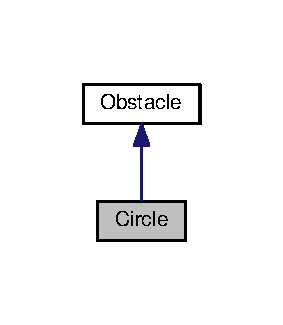
\includegraphics[width=136pt]{classCircle__inherit__graph}
\end{center}
\end{figure}


Collaboration diagram for Circle\+:\nopagebreak
\begin{figure}[H]
\begin{center}
\leavevmode
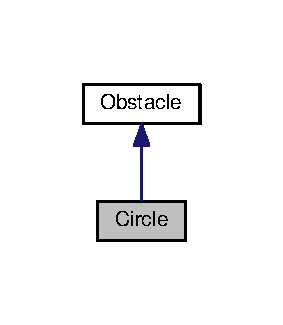
\includegraphics[width=136pt]{classCircle__coll__graph}
\end{center}
\end{figure}
\subsection*{Public Member Functions}
\begin{DoxyCompactItemize}
\item 
\hyperlink{classCircle_ad1ecfcfc7bf34529c6a6d6c448bf70fe}{Circle} ()
\begin{DoxyCompactList}\small\item\em Constructor to initialize all variables for obstacle class. \end{DoxyCompactList}\item 
void \hyperlink{classCircle_ad74925eb7a24bebd81cbef04ee174e6e}{set\+Boundary} (std\+::istream \&in, std\+::ostream \&out)
\begin{DoxyCompactList}\small\item\em Gets boundary of circle obstacle form user and updates the object. \end{DoxyCompactList}\item 
void \hyperlink{classCircle_a4c8e70958920c83bffcf316e3f3245b0}{disp\+Boundary} (std\+::ostream \&out)
\begin{DoxyCompactList}\small\item\em Display the circle obstacle boundary points to user that has given. \end{DoxyCompactList}\item 
bool \hyperlink{classCircle_ab2f11acd5263f4918b43608bc8eeb076}{in\+Obstacle} (int x\+Coord, int y\+Coord)
\begin{DoxyCompactList}\small\item\em Checks if the point is inside the circle obstacle. \end{DoxyCompactList}\item 
void \hyperlink{classCircle_a9e6224627d024141c53262844230fcbd}{fill\+Obstacle} (std\+::vector$<$ \hyperlink{structpoint}{point} $>$ \&ob\+Map)
\begin{DoxyCompactList}\small\item\em Finds all points in circle obstacle. \end{DoxyCompactList}\item 
virtual \hyperlink{classCircle_ae3f30436e645d73e368e8ee55f8d1650}{$\sim$\+Circle} ()
\begin{DoxyCompactList}\small\item\em Destructor to free up space once object goes out of scope. \end{DoxyCompactList}\end{DoxyCompactItemize}


\subsection{Detailed Description}
\hyperlink{classCircle}{Circle} class that holds functions of circular obstacle. 

\subsection{Constructor \& Destructor Documentation}
\index{Circle@{Circle}!Circle@{Circle}}
\index{Circle@{Circle}!Circle@{Circle}}
\subsubsection[{\texorpdfstring{Circle()}{Circle()}}]{\setlength{\rightskip}{0pt plus 5cm}Circle\+::\+Circle (
\begin{DoxyParamCaption}
{}
\end{DoxyParamCaption}
)}\hypertarget{classCircle_ad1ecfcfc7bf34529c6a6d6c448bf70fe}{}\label{classCircle_ad1ecfcfc7bf34529c6a6d6c448bf70fe}


Constructor to initialize all variables for obstacle class. 


\begin{DoxyParams}{Parameters}
{\em None} & \\
\hline
\end{DoxyParams}
\begin{DoxyReturn}{Returns}
None 
\end{DoxyReturn}
\index{Circle@{Circle}!````~Circle@{$\sim$\+Circle}}
\index{````~Circle@{$\sim$\+Circle}!Circle@{Circle}}
\subsubsection[{\texorpdfstring{$\sim$\+Circle()}{~Circle()}}]{\setlength{\rightskip}{0pt plus 5cm}Circle\+::$\sim$\+Circle (
\begin{DoxyParamCaption}
{}
\end{DoxyParamCaption}
)\hspace{0.3cm}{\ttfamily [virtual]}}\hypertarget{classCircle_ae3f30436e645d73e368e8ee55f8d1650}{}\label{classCircle_ae3f30436e645d73e368e8ee55f8d1650}


Destructor to free up space once object goes out of scope. 


\begin{DoxyParams}{Parameters}
{\em None} & \\
\hline
\end{DoxyParams}
\begin{DoxyReturn}{Returns}
None 
\end{DoxyReturn}


\subsection{Member Function Documentation}
\index{Circle@{Circle}!disp\+Boundary@{disp\+Boundary}}
\index{disp\+Boundary@{disp\+Boundary}!Circle@{Circle}}
\subsubsection[{\texorpdfstring{disp\+Boundary(std\+::ostream \&out)}{dispBoundary(std::ostream &out)}}]{\setlength{\rightskip}{0pt plus 5cm}void Circle\+::disp\+Boundary (
\begin{DoxyParamCaption}
\item[{std\+::ostream \&}]{out}
\end{DoxyParamCaption}
)\hspace{0.3cm}{\ttfamily [virtual]}}\hypertarget{classCircle_a4c8e70958920c83bffcf316e3f3245b0}{}\label{classCircle_a4c8e70958920c83bffcf316e3f3245b0}


Display the circle obstacle boundary points to user that has given. 


\begin{DoxyParams}{Parameters}
{\em Output} & stream \\
\hline
\end{DoxyParams}
\begin{DoxyReturn}{Returns}
input stream 
\end{DoxyReturn}


Implements \hyperlink{classObstacle_aba2625490b7d32632d585198038d279a}{Obstacle}.

\index{Circle@{Circle}!fill\+Obstacle@{fill\+Obstacle}}
\index{fill\+Obstacle@{fill\+Obstacle}!Circle@{Circle}}
\subsubsection[{\texorpdfstring{fill\+Obstacle(std\+::vector$<$ point $>$ \&ob\+Map)}{fillObstacle(std::vector< point > &obMap)}}]{\setlength{\rightskip}{0pt plus 5cm}void Circle\+::fill\+Obstacle (
\begin{DoxyParamCaption}
\item[{std\+::vector$<$ {\bf point} $>$ \&}]{ob\+Map}
\end{DoxyParamCaption}
)\hspace{0.3cm}{\ttfamily [virtual]}}\hypertarget{classCircle_a9e6224627d024141c53262844230fcbd}{}\label{classCircle_a9e6224627d024141c53262844230fcbd}


Finds all points in circle obstacle. 


\begin{DoxyParams}{Parameters}
{\em Vector} & to hold all points of obstacle \\
\hline
\end{DoxyParams}
\begin{DoxyReturn}{Returns}
None 
\end{DoxyReturn}


Implements \hyperlink{classObstacle_ade69ded6cb0d58ff914e64aaef4a0464}{Obstacle}.

\index{Circle@{Circle}!in\+Obstacle@{in\+Obstacle}}
\index{in\+Obstacle@{in\+Obstacle}!Circle@{Circle}}
\subsubsection[{\texorpdfstring{in\+Obstacle(int x\+Coord, int y\+Coord)}{inObstacle(int xCoord, int yCoord)}}]{\setlength{\rightskip}{0pt plus 5cm}bool Circle\+::in\+Obstacle (
\begin{DoxyParamCaption}
\item[{int}]{x\+Coord, }
\item[{int}]{y\+Coord}
\end{DoxyParamCaption}
)\hspace{0.3cm}{\ttfamily [virtual]}}\hypertarget{classCircle_ab2f11acd5263f4918b43608bc8eeb076}{}\label{classCircle_ab2f11acd5263f4918b43608bc8eeb076}


Checks if the point is inside the circle obstacle. 


\begin{DoxyParams}{Parameters}
{\em X} & and y coordinates for the point to be checked \\
\hline
\end{DoxyParams}
\begin{DoxyReturn}{Returns}
True if the point is inside obstacle else false 
\end{DoxyReturn}


Implements \hyperlink{classObstacle_a52c373a98616f6c41058f725b73479f5}{Obstacle}.

\index{Circle@{Circle}!set\+Boundary@{set\+Boundary}}
\index{set\+Boundary@{set\+Boundary}!Circle@{Circle}}
\subsubsection[{\texorpdfstring{set\+Boundary(std\+::istream \&in, std\+::ostream \&out)}{setBoundary(std::istream &in, std::ostream &out)}}]{\setlength{\rightskip}{0pt plus 5cm}void Circle\+::set\+Boundary (
\begin{DoxyParamCaption}
\item[{std\+::istream \&}]{in, }
\item[{std\+::ostream \&}]{out}
\end{DoxyParamCaption}
)\hspace{0.3cm}{\ttfamily [virtual]}}\hypertarget{classCircle_ad74925eb7a24bebd81cbef04ee174e6e}{}\label{classCircle_ad74925eb7a24bebd81cbef04ee174e6e}


Gets boundary of circle obstacle form user and updates the object. 


\begin{DoxyParams}{Parameters}
{\em Input} & and output stream \\
\hline
\end{DoxyParams}
\begin{DoxyReturn}{Returns}
None 
\end{DoxyReturn}


Implements \hyperlink{classObstacle_a8915ad90dc24f48df3ff0c38e8c695aa}{Obstacle}.



The documentation for this class was generated from the following files\+:\begin{DoxyCompactItemize}
\item 
/home/bala/workspace/\+Midterm project/\+C\+P\+P-\/\+R\+R\+T/include/\hyperlink{Circle_8h}{Circle.\+h}\item 
/home/bala/workspace/\+Midterm project/\+C\+P\+P-\/\+R\+R\+T/app/\hyperlink{Circle_8cpp}{Circle.\+cpp}\end{DoxyCompactItemize}

\hypertarget{structCircleTest}{}\section{Circle\+Test Struct Reference}
\label{structCircleTest}\index{Circle\+Test@{Circle\+Test}}


\hyperlink{classCircle}{Circle} class test fixture.  




Inheritance diagram for Circle\+Test\+:
\nopagebreak
\begin{figure}[H]
\begin{center}
\leavevmode
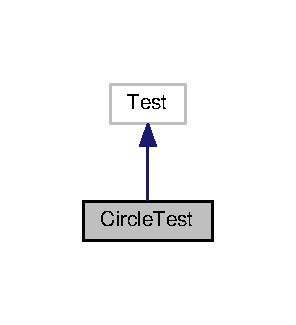
\includegraphics[width=142pt]{structCircleTest__inherit__graph}
\end{center}
\end{figure}


Collaboration diagram for Circle\+Test\+:
\nopagebreak
\begin{figure}[H]
\begin{center}
\leavevmode
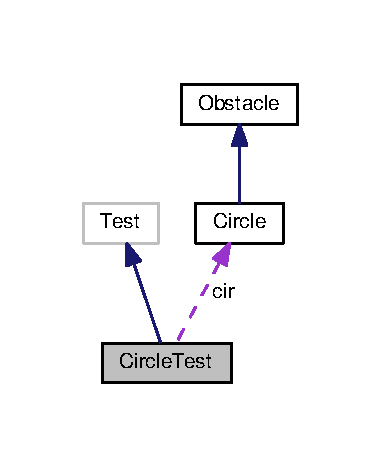
\includegraphics[width=183pt]{structCircleTest__coll__graph}
\end{center}
\end{figure}
\subsection*{Public Member Functions}
\begin{DoxyCompactItemize}
\item 
void \hyperlink{structCircleTest_a57ef2225672262bbee9911bb0f249212}{Set\+Up} ()
\item 
void \hyperlink{structCircleTest_a77a5186daec84ff2c67d44d3464783e0}{Tear\+Down} ()
\end{DoxyCompactItemize}
\subsection*{Public Attributes}
\begin{DoxyCompactItemize}
\item 
\hyperlink{classCircle}{Circle} $\ast$ \hyperlink{structCircleTest_aa15185e431282de6d6480bffde3f2be3}{cir}
\end{DoxyCompactItemize}


\subsection{Detailed Description}
\hyperlink{classCircle}{Circle} class test fixture. 

\subsection{Member Function Documentation}
\index{Circle\+Test@{Circle\+Test}!Set\+Up@{Set\+Up}}
\index{Set\+Up@{Set\+Up}!Circle\+Test@{Circle\+Test}}
\subsubsection[{\texorpdfstring{Set\+Up()}{SetUp()}}]{\setlength{\rightskip}{0pt plus 5cm}void Circle\+Test\+::\+Set\+Up (
\begin{DoxyParamCaption}
{}
\end{DoxyParamCaption}
)\hspace{0.3cm}{\ttfamily [inline]}}\hypertarget{structCircleTest_a57ef2225672262bbee9911bb0f249212}{}\label{structCircleTest_a57ef2225672262bbee9911bb0f249212}
\index{Circle\+Test@{Circle\+Test}!Tear\+Down@{Tear\+Down}}
\index{Tear\+Down@{Tear\+Down}!Circle\+Test@{Circle\+Test}}
\subsubsection[{\texorpdfstring{Tear\+Down()}{TearDown()}}]{\setlength{\rightskip}{0pt plus 5cm}void Circle\+Test\+::\+Tear\+Down (
\begin{DoxyParamCaption}
{}
\end{DoxyParamCaption}
)\hspace{0.3cm}{\ttfamily [inline]}}\hypertarget{structCircleTest_a77a5186daec84ff2c67d44d3464783e0}{}\label{structCircleTest_a77a5186daec84ff2c67d44d3464783e0}


\subsection{Member Data Documentation}
\index{Circle\+Test@{Circle\+Test}!cir@{cir}}
\index{cir@{cir}!Circle\+Test@{Circle\+Test}}
\subsubsection[{\texorpdfstring{cir}{cir}}]{\setlength{\rightskip}{0pt plus 5cm}{\bf Circle}$\ast$ Circle\+Test\+::cir}\hypertarget{structCircleTest_aa15185e431282de6d6480bffde3f2be3}{}\label{structCircleTest_aa15185e431282de6d6480bffde3f2be3}


The documentation for this struct was generated from the following file\+:\begin{DoxyCompactItemize}
\item 
/home/bala/workspace/\+Midterm project/\+C\+P\+P-\/\+R\+R\+T/test/\hyperlink{ObstacleTest_8cpp}{Obstacle\+Test.\+cpp}\end{DoxyCompactItemize}

\hypertarget{classInputMap}{}\section{Input\+Map Class Reference}
\label{classInputMap}\index{Input\+Map@{Input\+Map}}


Class holds map properties.  




{\ttfamily \#include $<$Input\+Map.\+h$>$}

\subsection*{Public Member Functions}
\begin{DoxyCompactItemize}
\item 
\hyperlink{classInputMap_aa79c436a267244b2151a564a56ac8b38}{Input\+Map} ()
\begin{DoxyCompactList}\small\item\em Constructor to initialize all variables. \end{DoxyCompactList}\item 
void \hyperlink{classInputMap_a5a60fff36f356c56c3787ffd1f7c05a2}{set\+Workspace} (std\+::shared\+\_\+ptr$<$ \hyperlink{classRobotWorkspace}{Robot\+Workspace} $>$ ws\+\_\+)
\begin{DoxyCompactList}\small\item\em Gets workspace parameters from user. \end{DoxyCompactList}\item 
void \hyperlink{classInputMap_a7a9eebead6fa8ebf4967c67c4b40db97}{add\+Obstacle} (std\+::vector$<$ std\+::shared\+\_\+ptr$<$ \hyperlink{classObstacle}{Obstacle} $>$$>$ \&ob\+\_\+)
\begin{DoxyCompactList}\small\item\em Adds all obstacles to inputmap object. \end{DoxyCompactList}\item 
void \hyperlink{classInputMap_a156a93dc41197c553f85e1b3634298ed}{compute\+Config\+Space} ()
\begin{DoxyCompactList}\small\item\em Compute free spaces in workspace. \end{DoxyCompactList}\item 
void \hyperlink{classInputMap_a98e7e9db9901085b4c3796a3e4757eff}{disp\+Config\+Space} (std\+::ostream \&out)
\begin{DoxyCompactList}\small\item\em Displays configuration points to user. \end{DoxyCompactList}\item 
virtual \hyperlink{classInputMap_a6f246c9507a85fd0ea168f5c72a2912e}{$\sim$\+Input\+Map} ()
\begin{DoxyCompactList}\small\item\em Destructor to free up space once object goes out of scope. \end{DoxyCompactList}\end{DoxyCompactItemize}
\subsection*{Public Attributes}
\begin{DoxyCompactItemize}
\item 
std\+::vector$<$ std\+::shared\+\_\+ptr$<$ \hyperlink{classObstacle}{Obstacle} $>$ $>$ \hyperlink{classInputMap_af0905398b4d3281f9876ff27350f9c3b}{ob}
\item 
std\+::shared\+\_\+ptr$<$ \hyperlink{classRobotWorkspace}{Robot\+Workspace} $>$ \hyperlink{classInputMap_aea6d53c88c8c0353dd7dc44fd295e256}{ws}
\item 
std\+::vector$<$ \hyperlink{structpoint}{point} $>$ \hyperlink{classInputMap_a2de100d8c53620d90aae543617a4e986}{config\+Space}
\end{DoxyCompactItemize}


\subsection{Detailed Description}
Class holds map properties. 

Map properties like obstacles, start point, goal point are stored here 

\subsection{Constructor \& Destructor Documentation}
\index{Input\+Map@{Input\+Map}!Input\+Map@{Input\+Map}}
\index{Input\+Map@{Input\+Map}!Input\+Map@{Input\+Map}}
\subsubsection[{\texorpdfstring{Input\+Map()}{InputMap()}}]{\setlength{\rightskip}{0pt plus 5cm}Input\+Map\+::\+Input\+Map (
\begin{DoxyParamCaption}
{}
\end{DoxyParamCaption}
)}\hypertarget{classInputMap_aa79c436a267244b2151a564a56ac8b38}{}\label{classInputMap_aa79c436a267244b2151a564a56ac8b38}


Constructor to initialize all variables. 


\begin{DoxyParams}{Parameters}
{\em None} & \\
\hline
\end{DoxyParams}
\begin{DoxyReturn}{Returns}
None 
\end{DoxyReturn}
\index{Input\+Map@{Input\+Map}!````~Input\+Map@{$\sim$\+Input\+Map}}
\index{````~Input\+Map@{$\sim$\+Input\+Map}!Input\+Map@{Input\+Map}}
\subsubsection[{\texorpdfstring{$\sim$\+Input\+Map()}{~InputMap()}}]{\setlength{\rightskip}{0pt plus 5cm}Input\+Map\+::$\sim$\+Input\+Map (
\begin{DoxyParamCaption}
{}
\end{DoxyParamCaption}
)\hspace{0.3cm}{\ttfamily [virtual]}}\hypertarget{classInputMap_a6f246c9507a85fd0ea168f5c72a2912e}{}\label{classInputMap_a6f246c9507a85fd0ea168f5c72a2912e}


Destructor to free up space once object goes out of scope. 


\begin{DoxyParams}{Parameters}
{\em None} & \\
\hline
\end{DoxyParams}
\begin{DoxyReturn}{Returns}
None 
\end{DoxyReturn}


\subsection{Member Function Documentation}
\index{Input\+Map@{Input\+Map}!add\+Obstacle@{add\+Obstacle}}
\index{add\+Obstacle@{add\+Obstacle}!Input\+Map@{Input\+Map}}
\subsubsection[{\texorpdfstring{add\+Obstacle(std\+::vector$<$ std\+::shared\+\_\+ptr$<$ Obstacle $>$$>$ \&ob\+\_\+)}{addObstacle(std::vector< std::shared_ptr< Obstacle >> &ob_)}}]{\setlength{\rightskip}{0pt plus 5cm}void Input\+Map\+::add\+Obstacle (
\begin{DoxyParamCaption}
\item[{std\+::vector$<$ std\+::shared\+\_\+ptr$<$ {\bf Obstacle} $>$$>$ \&}]{ob\+\_\+}
\end{DoxyParamCaption}
)}\hypertarget{classInputMap_a7a9eebead6fa8ebf4967c67c4b40db97}{}\label{classInputMap_a7a9eebead6fa8ebf4967c67c4b40db97}


Adds all obstacles to inputmap object. 


\begin{DoxyParams}{Parameters}
{\em Vector} & of obstacles \\
\hline
\end{DoxyParams}
\begin{DoxyReturn}{Returns}
None 
\end{DoxyReturn}
\index{Input\+Map@{Input\+Map}!compute\+Config\+Space@{compute\+Config\+Space}}
\index{compute\+Config\+Space@{compute\+Config\+Space}!Input\+Map@{Input\+Map}}
\subsubsection[{\texorpdfstring{compute\+Config\+Space()}{computeConfigSpace()}}]{\setlength{\rightskip}{0pt plus 5cm}void Input\+Map\+::compute\+Config\+Space (
\begin{DoxyParamCaption}
{}
\end{DoxyParamCaption}
)}\hypertarget{classInputMap_a156a93dc41197c553f85e1b3634298ed}{}\label{classInputMap_a156a93dc41197c553f85e1b3634298ed}


Compute free spaces in workspace. 


\begin{DoxyParams}{Parameters}
{\em None} & \\
\hline
\end{DoxyParams}
\begin{DoxyReturn}{Returns}
None 
\end{DoxyReturn}
\index{Input\+Map@{Input\+Map}!disp\+Config\+Space@{disp\+Config\+Space}}
\index{disp\+Config\+Space@{disp\+Config\+Space}!Input\+Map@{Input\+Map}}
\subsubsection[{\texorpdfstring{disp\+Config\+Space(std\+::ostream \&out)}{dispConfigSpace(std::ostream &out)}}]{\setlength{\rightskip}{0pt plus 5cm}void Input\+Map\+::disp\+Config\+Space (
\begin{DoxyParamCaption}
\item[{std\+::ostream \&}]{out}
\end{DoxyParamCaption}
)}\hypertarget{classInputMap_a98e7e9db9901085b4c3796a3e4757eff}{}\label{classInputMap_a98e7e9db9901085b4c3796a3e4757eff}


Displays configuration points to user. 


\begin{DoxyParams}{Parameters}
{\em Output} & stream reference \\
\hline
\end{DoxyParams}
\begin{DoxyReturn}{Returns}
None 
\end{DoxyReturn}
\index{Input\+Map@{Input\+Map}!set\+Workspace@{set\+Workspace}}
\index{set\+Workspace@{set\+Workspace}!Input\+Map@{Input\+Map}}
\subsubsection[{\texorpdfstring{set\+Workspace(std\+::shared\+\_\+ptr$<$ Robot\+Workspace $>$ ws\+\_\+)}{setWorkspace(std::shared_ptr< RobotWorkspace > ws_)}}]{\setlength{\rightskip}{0pt plus 5cm}void Input\+Map\+::set\+Workspace (
\begin{DoxyParamCaption}
\item[{std\+::shared\+\_\+ptr$<$ {\bf Robot\+Workspace} $>$}]{ws\+\_\+}
\end{DoxyParamCaption}
)}\hypertarget{classInputMap_a5a60fff36f356c56c3787ffd1f7c05a2}{}\label{classInputMap_a5a60fff36f356c56c3787ffd1f7c05a2}


Gets workspace parameters from user. 


\begin{DoxyParams}{Parameters}
{\em shared} & pointer to workspace objec \\
\hline
\end{DoxyParams}
\begin{DoxyReturn}{Returns}
None 
\end{DoxyReturn}


\subsection{Member Data Documentation}
\index{Input\+Map@{Input\+Map}!config\+Space@{config\+Space}}
\index{config\+Space@{config\+Space}!Input\+Map@{Input\+Map}}
\subsubsection[{\texorpdfstring{config\+Space}{configSpace}}]{\setlength{\rightskip}{0pt plus 5cm}std\+::vector$<${\bf point}$>$ Input\+Map\+::config\+Space}\hypertarget{classInputMap_a2de100d8c53620d90aae543617a4e986}{}\label{classInputMap_a2de100d8c53620d90aae543617a4e986}
\index{Input\+Map@{Input\+Map}!ob@{ob}}
\index{ob@{ob}!Input\+Map@{Input\+Map}}
\subsubsection[{\texorpdfstring{ob}{ob}}]{\setlength{\rightskip}{0pt plus 5cm}std\+::vector$<$std\+::shared\+\_\+ptr$<${\bf Obstacle}$>$ $>$ Input\+Map\+::ob}\hypertarget{classInputMap_af0905398b4d3281f9876ff27350f9c3b}{}\label{classInputMap_af0905398b4d3281f9876ff27350f9c3b}
\index{Input\+Map@{Input\+Map}!ws@{ws}}
\index{ws@{ws}!Input\+Map@{Input\+Map}}
\subsubsection[{\texorpdfstring{ws}{ws}}]{\setlength{\rightskip}{0pt plus 5cm}std\+::shared\+\_\+ptr$<${\bf Robot\+Workspace}$>$ Input\+Map\+::ws}\hypertarget{classInputMap_aea6d53c88c8c0353dd7dc44fd295e256}{}\label{classInputMap_aea6d53c88c8c0353dd7dc44fd295e256}


The documentation for this class was generated from the following files\+:\begin{DoxyCompactItemize}
\item 
/home/bala/workspace/\+Midterm project/\+C\+P\+P-\/\+R\+R\+T/include/\hyperlink{InputMap_8h}{Input\+Map.\+h}\item 
/home/bala/workspace/\+Midterm project/\+C\+P\+P-\/\+R\+R\+T/app/\hyperlink{InputMap_8cpp}{Input\+Map.\+cpp}\end{DoxyCompactItemize}

\hypertarget{classObstacle}{}\section{Obstacle Class Reference}
\label{classObstacle}\index{Obstacle@{Obstacle}}


\hyperlink{classObstacle}{Obstacle} obstacle class that serves as parent for all types of obstacles.  




{\ttfamily \#include $<$Obstacle.\+h$>$}



Inheritance diagram for Obstacle\+:\nopagebreak
\begin{figure}[H]
\begin{center}
\leavevmode
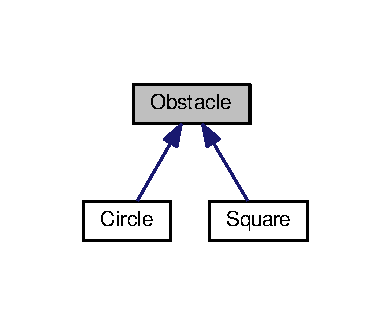
\includegraphics[width=188pt]{classObstacle__inherit__graph}
\end{center}
\end{figure}
\subsection*{Public Member Functions}
\begin{DoxyCompactItemize}
\item 
\hyperlink{classObstacle_a8f734072321fa06a7b7dae2d5f50f352}{Obstacle} ()
\begin{DoxyCompactList}\small\item\em Constructor to initialize all variables for obstacle class. \end{DoxyCompactList}\item 
virtual void \hyperlink{classObstacle_a8915ad90dc24f48df3ff0c38e8c695aa}{set\+Boundary} (std\+::istream \&in, std\+::ostream \&out)=0
\begin{DoxyCompactList}\small\item\em Virtual function that gets boundary of obstacle form user and updates the object. \end{DoxyCompactList}\item 
virtual void \hyperlink{classObstacle_aba2625490b7d32632d585198038d279a}{disp\+Boundary} (std\+::ostream \&out)=0
\begin{DoxyCompactList}\small\item\em Virtual function to display the obstacle boundary points to user that has given. \end{DoxyCompactList}\item 
virtual bool \hyperlink{classObstacle_a52c373a98616f6c41058f725b73479f5}{in\+Obstacle} (int x\+Coord, int y\+Coord)=0
\begin{DoxyCompactList}\small\item\em Finds all points in obstacle. \end{DoxyCompactList}\item 
virtual void \hyperlink{classObstacle_ade69ded6cb0d58ff914e64aaef4a0464}{fill\+Obstacle} (std\+::vector$<$ \hyperlink{structpoint}{point} $>$ \&ob\+Map)=0
\begin{DoxyCompactList}\small\item\em Virtual function to find all points in obstacle. \end{DoxyCompactList}\item 
virtual \hyperlink{classObstacle_af2f9cc9c6cff75dca0974fd5ac4f71a9}{$\sim$\+Obstacle} ()
\begin{DoxyCompactList}\small\item\em Destructor to free up space once object goes out of scope. \end{DoxyCompactList}\end{DoxyCompactItemize}


\subsection{Detailed Description}
\hyperlink{classObstacle}{Obstacle} obstacle class that serves as parent for all types of obstacles. 

\subsection{Constructor \& Destructor Documentation}
\index{Obstacle@{Obstacle}!Obstacle@{Obstacle}}
\index{Obstacle@{Obstacle}!Obstacle@{Obstacle}}
\subsubsection[{\texorpdfstring{Obstacle()}{Obstacle()}}]{\setlength{\rightskip}{0pt plus 5cm}Obstacle\+::\+Obstacle (
\begin{DoxyParamCaption}
{}
\end{DoxyParamCaption}
)}\hypertarget{classObstacle_a8f734072321fa06a7b7dae2d5f50f352}{}\label{classObstacle_a8f734072321fa06a7b7dae2d5f50f352}


Constructor to initialize all variables for obstacle class. 


\begin{DoxyParams}{Parameters}
{\em None} & \\
\hline
\end{DoxyParams}
\begin{DoxyReturn}{Returns}
None 
\end{DoxyReturn}
\index{Obstacle@{Obstacle}!````~Obstacle@{$\sim$\+Obstacle}}
\index{````~Obstacle@{$\sim$\+Obstacle}!Obstacle@{Obstacle}}
\subsubsection[{\texorpdfstring{$\sim$\+Obstacle()}{~Obstacle()}}]{\setlength{\rightskip}{0pt plus 5cm}Obstacle\+::$\sim$\+Obstacle (
\begin{DoxyParamCaption}
{}
\end{DoxyParamCaption}
)\hspace{0.3cm}{\ttfamily [virtual]}}\hypertarget{classObstacle_af2f9cc9c6cff75dca0974fd5ac4f71a9}{}\label{classObstacle_af2f9cc9c6cff75dca0974fd5ac4f71a9}


Destructor to free up space once object goes out of scope. 


\begin{DoxyParams}{Parameters}
{\em None} & \\
\hline
\end{DoxyParams}
\begin{DoxyReturn}{Returns}
None 
\end{DoxyReturn}


\subsection{Member Function Documentation}
\index{Obstacle@{Obstacle}!disp\+Boundary@{disp\+Boundary}}
\index{disp\+Boundary@{disp\+Boundary}!Obstacle@{Obstacle}}
\subsubsection[{\texorpdfstring{disp\+Boundary(std\+::ostream \&out)=0}{dispBoundary(std::ostream &out)=0}}]{\setlength{\rightskip}{0pt plus 5cm}virtual void Obstacle\+::disp\+Boundary (
\begin{DoxyParamCaption}
\item[{std\+::ostream \&}]{out}
\end{DoxyParamCaption}
)\hspace{0.3cm}{\ttfamily [pure virtual]}}\hypertarget{classObstacle_aba2625490b7d32632d585198038d279a}{}\label{classObstacle_aba2625490b7d32632d585198038d279a}


Virtual function to display the obstacle boundary points to user that has given. 


\begin{DoxyParams}{Parameters}
{\em Output} & stream \\
\hline
\end{DoxyParams}
\begin{DoxyReturn}{Returns}
input stream 
\end{DoxyReturn}


Implemented in \hyperlink{classCircle_a4c8e70958920c83bffcf316e3f3245b0}{Circle}, and \hyperlink{classSquare_afb76b9979da299090aa92f7e02465843}{Square}.

\index{Obstacle@{Obstacle}!fill\+Obstacle@{fill\+Obstacle}}
\index{fill\+Obstacle@{fill\+Obstacle}!Obstacle@{Obstacle}}
\subsubsection[{\texorpdfstring{fill\+Obstacle(std\+::vector$<$ point $>$ \&ob\+Map)=0}{fillObstacle(std::vector< point > &obMap)=0}}]{\setlength{\rightskip}{0pt plus 5cm}virtual void Obstacle\+::fill\+Obstacle (
\begin{DoxyParamCaption}
\item[{std\+::vector$<$ {\bf point} $>$ \&}]{ob\+Map}
\end{DoxyParamCaption}
)\hspace{0.3cm}{\ttfamily [pure virtual]}}\hypertarget{classObstacle_ade69ded6cb0d58ff914e64aaef4a0464}{}\label{classObstacle_ade69ded6cb0d58ff914e64aaef4a0464}


Virtual function to find all points in obstacle. 


\begin{DoxyParams}{Parameters}
{\em Vector} & to hold all points of obstacle \\
\hline
\end{DoxyParams}
\begin{DoxyReturn}{Returns}
None 
\end{DoxyReturn}


Implemented in \hyperlink{classCircle_a9e6224627d024141c53262844230fcbd}{Circle}, and \hyperlink{classSquare_a395dc9319c9609d810e3f22eddbdcc81}{Square}.

\index{Obstacle@{Obstacle}!in\+Obstacle@{in\+Obstacle}}
\index{in\+Obstacle@{in\+Obstacle}!Obstacle@{Obstacle}}
\subsubsection[{\texorpdfstring{in\+Obstacle(int x\+Coord, int y\+Coord)=0}{inObstacle(int xCoord, int yCoord)=0}}]{\setlength{\rightskip}{0pt plus 5cm}virtual bool Obstacle\+::in\+Obstacle (
\begin{DoxyParamCaption}
\item[{int}]{x\+Coord, }
\item[{int}]{y\+Coord}
\end{DoxyParamCaption}
)\hspace{0.3cm}{\ttfamily [pure virtual]}}\hypertarget{classObstacle_a52c373a98616f6c41058f725b73479f5}{}\label{classObstacle_a52c373a98616f6c41058f725b73479f5}


Finds all points in obstacle. 


\begin{DoxyParams}{Parameters}
{\em Vector} & to hold all points of obstacle \\
\hline
\end{DoxyParams}
\begin{DoxyReturn}{Returns}
None 
\end{DoxyReturn}


Implemented in \hyperlink{classCircle_ab2f11acd5263f4918b43608bc8eeb076}{Circle}, and \hyperlink{classSquare_aa07ba26ea5675fea6dc90b2172ab13dd}{Square}.

\index{Obstacle@{Obstacle}!set\+Boundary@{set\+Boundary}}
\index{set\+Boundary@{set\+Boundary}!Obstacle@{Obstacle}}
\subsubsection[{\texorpdfstring{set\+Boundary(std\+::istream \&in, std\+::ostream \&out)=0}{setBoundary(std::istream &in, std::ostream &out)=0}}]{\setlength{\rightskip}{0pt plus 5cm}virtual void Obstacle\+::set\+Boundary (
\begin{DoxyParamCaption}
\item[{std\+::istream \&}]{in, }
\item[{std\+::ostream \&}]{out}
\end{DoxyParamCaption}
)\hspace{0.3cm}{\ttfamily [pure virtual]}}\hypertarget{classObstacle_a8915ad90dc24f48df3ff0c38e8c695aa}{}\label{classObstacle_a8915ad90dc24f48df3ff0c38e8c695aa}


Virtual function that gets boundary of obstacle form user and updates the object. 


\begin{DoxyParams}{Parameters}
{\em Input} & and output stream \\
\hline
\end{DoxyParams}
\begin{DoxyReturn}{Returns}
None 
\end{DoxyReturn}


Implemented in \hyperlink{classCircle_ad74925eb7a24bebd81cbef04ee174e6e}{Circle}, and \hyperlink{classSquare_a1979921c7ae05d518c4392e0d5b8c156}{Square}.



The documentation for this class was generated from the following files\+:\begin{DoxyCompactItemize}
\item 
/home/bala/workspace/\+Midterm project/\+C\+P\+P-\/\+R\+R\+T/include/\hyperlink{Obstacle_8h}{Obstacle.\+h}\item 
/home/bala/workspace/\+Midterm project/\+C\+P\+P-\/\+R\+R\+T/app/\hyperlink{Obstacle_8cpp}{Obstacle.\+cpp}\end{DoxyCompactItemize}

\hypertarget{structObstacleCircleTest}{}\section{Obstacle\+Circle\+Test Struct Reference}
\label{structObstacleCircleTest}\index{Obstacle\+Circle\+Test@{Obstacle\+Circle\+Test}}


\hyperlink{classObstacle}{Obstacle} \hyperlink{classCircle}{Circle} class test fixture for overriding.  




Inheritance diagram for Obstacle\+Circle\+Test\+:
\nopagebreak
\begin{figure}[H]
\begin{center}
\leavevmode
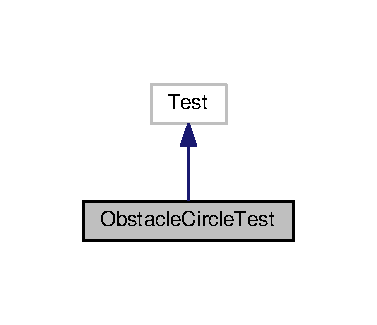
\includegraphics[width=181pt]{structObstacleCircleTest__inherit__graph}
\end{center}
\end{figure}


Collaboration diagram for Obstacle\+Circle\+Test\+:
\nopagebreak
\begin{figure}[H]
\begin{center}
\leavevmode
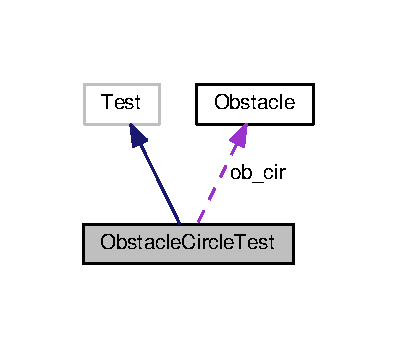
\includegraphics[width=191pt]{structObstacleCircleTest__coll__graph}
\end{center}
\end{figure}
\subsection*{Public Member Functions}
\begin{DoxyCompactItemize}
\item 
void \hyperlink{structObstacleCircleTest_a3f4cb1b05f4b820fb6042bd9278c516d}{Set\+Up} ()
\item 
void \hyperlink{structObstacleCircleTest_a994997c94bc7e1abc8055924051bcad6}{Tear\+Down} ()
\end{DoxyCompactItemize}
\subsection*{Public Attributes}
\begin{DoxyCompactItemize}
\item 
\hyperlink{classObstacle}{Obstacle} $\ast$ \hyperlink{structObstacleCircleTest_a6e3bfbeae582ed90e1d0c20f76b2156a}{ob\+\_\+cir}
\end{DoxyCompactItemize}


\subsection{Detailed Description}
\hyperlink{classObstacle}{Obstacle} \hyperlink{classCircle}{Circle} class test fixture for overriding. 

\subsection{Member Function Documentation}
\index{Obstacle\+Circle\+Test@{Obstacle\+Circle\+Test}!Set\+Up@{Set\+Up}}
\index{Set\+Up@{Set\+Up}!Obstacle\+Circle\+Test@{Obstacle\+Circle\+Test}}
\subsubsection[{\texorpdfstring{Set\+Up()}{SetUp()}}]{\setlength{\rightskip}{0pt plus 5cm}void Obstacle\+Circle\+Test\+::\+Set\+Up (
\begin{DoxyParamCaption}
{}
\end{DoxyParamCaption}
)\hspace{0.3cm}{\ttfamily [inline]}}\hypertarget{structObstacleCircleTest_a3f4cb1b05f4b820fb6042bd9278c516d}{}\label{structObstacleCircleTest_a3f4cb1b05f4b820fb6042bd9278c516d}
\index{Obstacle\+Circle\+Test@{Obstacle\+Circle\+Test}!Tear\+Down@{Tear\+Down}}
\index{Tear\+Down@{Tear\+Down}!Obstacle\+Circle\+Test@{Obstacle\+Circle\+Test}}
\subsubsection[{\texorpdfstring{Tear\+Down()}{TearDown()}}]{\setlength{\rightskip}{0pt plus 5cm}void Obstacle\+Circle\+Test\+::\+Tear\+Down (
\begin{DoxyParamCaption}
{}
\end{DoxyParamCaption}
)\hspace{0.3cm}{\ttfamily [inline]}}\hypertarget{structObstacleCircleTest_a994997c94bc7e1abc8055924051bcad6}{}\label{structObstacleCircleTest_a994997c94bc7e1abc8055924051bcad6}


\subsection{Member Data Documentation}
\index{Obstacle\+Circle\+Test@{Obstacle\+Circle\+Test}!ob\+\_\+cir@{ob\+\_\+cir}}
\index{ob\+\_\+cir@{ob\+\_\+cir}!Obstacle\+Circle\+Test@{Obstacle\+Circle\+Test}}
\subsubsection[{\texorpdfstring{ob\+\_\+cir}{ob_cir}}]{\setlength{\rightskip}{0pt plus 5cm}{\bf Obstacle}$\ast$ Obstacle\+Circle\+Test\+::ob\+\_\+cir}\hypertarget{structObstacleCircleTest_a6e3bfbeae582ed90e1d0c20f76b2156a}{}\label{structObstacleCircleTest_a6e3bfbeae582ed90e1d0c20f76b2156a}


The documentation for this struct was generated from the following file\+:\begin{DoxyCompactItemize}
\item 
/home/bala/workspace/\+Midterm project/\+C\+P\+P-\/\+R\+R\+T/test/\hyperlink{ObstacleTest_8cpp}{Obstacle\+Test.\+cpp}\end{DoxyCompactItemize}

\hypertarget{structObstacleSquareTest}{}\section{Obstacle\+Square\+Test Struct Reference}
\label{structObstacleSquareTest}\index{Obstacle\+Square\+Test@{Obstacle\+Square\+Test}}


\hyperlink{classObstacle}{Obstacle} square class test fixture for overriding.  




Inheritance diagram for Obstacle\+Square\+Test\+:
\nopagebreak
\begin{figure}[H]
\begin{center}
\leavevmode
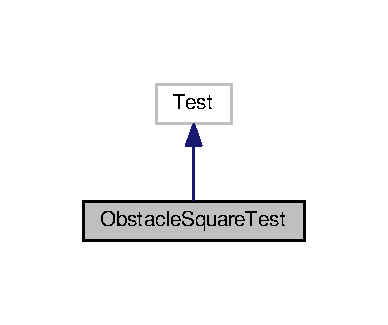
\includegraphics[width=186pt]{structObstacleSquareTest__inherit__graph}
\end{center}
\end{figure}


Collaboration diagram for Obstacle\+Square\+Test\+:
\nopagebreak
\begin{figure}[H]
\begin{center}
\leavevmode
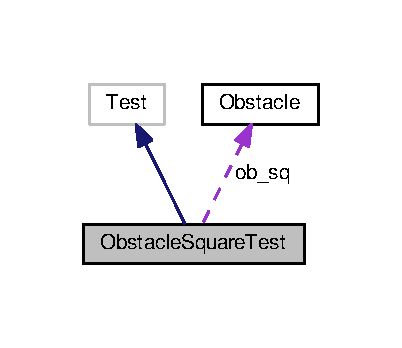
\includegraphics[width=193pt]{structObstacleSquareTest__coll__graph}
\end{center}
\end{figure}
\subsection*{Public Member Functions}
\begin{DoxyCompactItemize}
\item 
void \hyperlink{structObstacleSquareTest_a1b4031fb1b71d0b365037a7a0c32c75b}{Set\+Up} ()
\item 
void \hyperlink{structObstacleSquareTest_a45434f333e6c64f5cf9b2aa7814d8022}{Tear\+Down} ()
\end{DoxyCompactItemize}
\subsection*{Public Attributes}
\begin{DoxyCompactItemize}
\item 
\hyperlink{classObstacle}{Obstacle} $\ast$ \hyperlink{structObstacleSquareTest_a824c56e1d851328b7130e42d64b1c571}{ob\+\_\+sq}
\end{DoxyCompactItemize}


\subsection{Detailed Description}
\hyperlink{classObstacle}{Obstacle} square class test fixture for overriding. 

\subsection{Member Function Documentation}
\index{Obstacle\+Square\+Test@{Obstacle\+Square\+Test}!Set\+Up@{Set\+Up}}
\index{Set\+Up@{Set\+Up}!Obstacle\+Square\+Test@{Obstacle\+Square\+Test}}
\subsubsection[{\texorpdfstring{Set\+Up()}{SetUp()}}]{\setlength{\rightskip}{0pt plus 5cm}void Obstacle\+Square\+Test\+::\+Set\+Up (
\begin{DoxyParamCaption}
{}
\end{DoxyParamCaption}
)\hspace{0.3cm}{\ttfamily [inline]}}\hypertarget{structObstacleSquareTest_a1b4031fb1b71d0b365037a7a0c32c75b}{}\label{structObstacleSquareTest_a1b4031fb1b71d0b365037a7a0c32c75b}
\index{Obstacle\+Square\+Test@{Obstacle\+Square\+Test}!Tear\+Down@{Tear\+Down}}
\index{Tear\+Down@{Tear\+Down}!Obstacle\+Square\+Test@{Obstacle\+Square\+Test}}
\subsubsection[{\texorpdfstring{Tear\+Down()}{TearDown()}}]{\setlength{\rightskip}{0pt plus 5cm}void Obstacle\+Square\+Test\+::\+Tear\+Down (
\begin{DoxyParamCaption}
{}
\end{DoxyParamCaption}
)\hspace{0.3cm}{\ttfamily [inline]}}\hypertarget{structObstacleSquareTest_a45434f333e6c64f5cf9b2aa7814d8022}{}\label{structObstacleSquareTest_a45434f333e6c64f5cf9b2aa7814d8022}


\subsection{Member Data Documentation}
\index{Obstacle\+Square\+Test@{Obstacle\+Square\+Test}!ob\+\_\+sq@{ob\+\_\+sq}}
\index{ob\+\_\+sq@{ob\+\_\+sq}!Obstacle\+Square\+Test@{Obstacle\+Square\+Test}}
\subsubsection[{\texorpdfstring{ob\+\_\+sq}{ob_sq}}]{\setlength{\rightskip}{0pt plus 5cm}{\bf Obstacle}$\ast$ Obstacle\+Square\+Test\+::ob\+\_\+sq}\hypertarget{structObstacleSquareTest_a824c56e1d851328b7130e42d64b1c571}{}\label{structObstacleSquareTest_a824c56e1d851328b7130e42d64b1c571}


The documentation for this struct was generated from the following file\+:\begin{DoxyCompactItemize}
\item 
/home/bala/workspace/\+Midterm project/\+C\+P\+P-\/\+R\+R\+T/test/\hyperlink{ObstacleTest_8cpp}{Obstacle\+Test.\+cpp}\end{DoxyCompactItemize}

\hypertarget{classPathDisplay}{}\section{Path\+Display Class Reference}
\label{classPathDisplay}\index{Path\+Display@{Path\+Display}}


Class to display path along with arena to user.  




{\ttfamily \#include $<$Path\+Display.\+h$>$}

\subsection*{Public Member Functions}
\begin{DoxyCompactItemize}
\item 
\hyperlink{classPathDisplay_a53f5ac55c989347750fc401ced3355ed}{Path\+Display} ()
\begin{DoxyCompactList}\small\item\em Constructor to initialize all variables. \end{DoxyCompactList}\item 
void \hyperlink{classPathDisplay_ac1c4ea52e9ba7f73bd9a1569e8399575}{update\+Input\+Map} (std\+::shared\+\_\+ptr$<$ \hyperlink{classInputMap}{Input\+Map} $>$ \+\_\+i\+Map)
\begin{DoxyCompactList}\small\item\em Updates the input map object. \end{DoxyCompactList}\item 
void \hyperlink{classPathDisplay_a3dddc0af19261aaf8021551510009422}{display\+Path} (std\+::ostream \&out, std\+::vector$<$ \hyperlink{structpoint}{point} $>$ \&path)
\begin{DoxyCompactList}\small\item\em Displays path and robot arena to user. \end{DoxyCompactList}\item 
virtual \hyperlink{classPathDisplay_aa49d540a7706c1dff83e2fc9120d8d59}{$\sim$\+Path\+Display} ()
\begin{DoxyCompactList}\small\item\em Destructor to free up space once object goes out of scope. \end{DoxyCompactList}\end{DoxyCompactItemize}
\subsection*{Public Attributes}
\begin{DoxyCompactItemize}
\item 
std\+::shared\+\_\+ptr$<$ \hyperlink{classInputMap}{Input\+Map} $>$ \hyperlink{classPathDisplay_af35e969a46cc0a7c5ec013efde7ae51e}{i\+Map}
\end{DoxyCompactItemize}


\subsection{Detailed Description}
Class to display path along with arena to user. 

\subsection{Constructor \& Destructor Documentation}
\index{Path\+Display@{Path\+Display}!Path\+Display@{Path\+Display}}
\index{Path\+Display@{Path\+Display}!Path\+Display@{Path\+Display}}
\subsubsection[{\texorpdfstring{Path\+Display()}{PathDisplay()}}]{\setlength{\rightskip}{0pt plus 5cm}Path\+Display\+::\+Path\+Display (
\begin{DoxyParamCaption}
{}
\end{DoxyParamCaption}
)}\hypertarget{classPathDisplay_a53f5ac55c989347750fc401ced3355ed}{}\label{classPathDisplay_a53f5ac55c989347750fc401ced3355ed}


Constructor to initialize all variables. 


\begin{DoxyParams}{Parameters}
{\em None} & \\
\hline
\end{DoxyParams}
\begin{DoxyReturn}{Returns}
None 
\end{DoxyReturn}
\index{Path\+Display@{Path\+Display}!````~Path\+Display@{$\sim$\+Path\+Display}}
\index{````~Path\+Display@{$\sim$\+Path\+Display}!Path\+Display@{Path\+Display}}
\subsubsection[{\texorpdfstring{$\sim$\+Path\+Display()}{~PathDisplay()}}]{\setlength{\rightskip}{0pt plus 5cm}Path\+Display\+::$\sim$\+Path\+Display (
\begin{DoxyParamCaption}
{}
\end{DoxyParamCaption}
)\hspace{0.3cm}{\ttfamily [virtual]}}\hypertarget{classPathDisplay_aa49d540a7706c1dff83e2fc9120d8d59}{}\label{classPathDisplay_aa49d540a7706c1dff83e2fc9120d8d59}


Destructor to free up space once object goes out of scope. 


\begin{DoxyParams}{Parameters}
{\em None} & \\
\hline
\end{DoxyParams}
\begin{DoxyReturn}{Returns}
None 
\end{DoxyReturn}


\subsection{Member Function Documentation}
\index{Path\+Display@{Path\+Display}!display\+Path@{display\+Path}}
\index{display\+Path@{display\+Path}!Path\+Display@{Path\+Display}}
\subsubsection[{\texorpdfstring{display\+Path(std\+::ostream \&out, std\+::vector$<$ point $>$ \&path)}{displayPath(std::ostream &out, std::vector< point > &path)}}]{\setlength{\rightskip}{0pt plus 5cm}void Path\+Display\+::display\+Path (
\begin{DoxyParamCaption}
\item[{std\+::ostream \&}]{out, }
\item[{std\+::vector$<$ {\bf point} $>$ \&}]{path}
\end{DoxyParamCaption}
)}\hypertarget{classPathDisplay_a3dddc0af19261aaf8021551510009422}{}\label{classPathDisplay_a3dddc0af19261aaf8021551510009422}


Displays path and robot arena to user. 


\begin{DoxyParams}{Parameters}
{\em Input} & and output stream references \\
\hline
\end{DoxyParams}
\begin{DoxyReturn}{Returns}
None 
\end{DoxyReturn}
\index{Path\+Display@{Path\+Display}!update\+Input\+Map@{update\+Input\+Map}}
\index{update\+Input\+Map@{update\+Input\+Map}!Path\+Display@{Path\+Display}}
\subsubsection[{\texorpdfstring{update\+Input\+Map(std\+::shared\+\_\+ptr$<$ Input\+Map $>$ \+\_\+i\+Map)}{updateInputMap(std::shared_ptr< InputMap > _iMap)}}]{\setlength{\rightskip}{0pt plus 5cm}void Path\+Display\+::update\+Input\+Map (
\begin{DoxyParamCaption}
\item[{std\+::shared\+\_\+ptr$<$ {\bf Input\+Map} $>$}]{\+\_\+i\+Map}
\end{DoxyParamCaption}
)}\hypertarget{classPathDisplay_ac1c4ea52e9ba7f73bd9a1569e8399575}{}\label{classPathDisplay_ac1c4ea52e9ba7f73bd9a1569e8399575}


Updates the input map object. 


\begin{DoxyParams}{Parameters}
{\em Shared} & pointer to input map object \\
\hline
\end{DoxyParams}
\begin{DoxyReturn}{Returns}
None 
\end{DoxyReturn}


\subsection{Member Data Documentation}
\index{Path\+Display@{Path\+Display}!i\+Map@{i\+Map}}
\index{i\+Map@{i\+Map}!Path\+Display@{Path\+Display}}
\subsubsection[{\texorpdfstring{i\+Map}{iMap}}]{\setlength{\rightskip}{0pt plus 5cm}std\+::shared\+\_\+ptr$<${\bf Input\+Map}$>$ Path\+Display\+::i\+Map}\hypertarget{classPathDisplay_af35e969a46cc0a7c5ec013efde7ae51e}{}\label{classPathDisplay_af35e969a46cc0a7c5ec013efde7ae51e}


The documentation for this class was generated from the following files\+:\begin{DoxyCompactItemize}
\item 
/home/bala/workspace/\+Midterm project/\+C\+P\+P-\/\+R\+R\+T/include/\hyperlink{PathDisplay_8h}{Path\+Display.\+h}\item 
/home/bala/workspace/\+Midterm project/\+C\+P\+P-\/\+R\+R\+T/app/\hyperlink{PathDisplay_8cpp}{Path\+Display.\+cpp}\end{DoxyCompactItemize}

\hypertarget{structpoint}{}\section{point Struct Reference}
\label{structpoint}\index{point@{point}}


{\ttfamily \#include $<$Obstacle.\+h$>$}

\subsection*{Public Attributes}
\begin{DoxyCompactItemize}
\item 
int \hyperlink{structpoint_ad679b07fb69d55f5ad454d0f1f2891d5}{x}
\item 
int \hyperlink{structpoint_a9a82ca9504acabb1e30569f89c805471}{y}
\end{DoxyCompactItemize}


\subsection{Member Data Documentation}
\index{point@{point}!x@{x}}
\index{x@{x}!point@{point}}
\subsubsection[{\texorpdfstring{x}{x}}]{\setlength{\rightskip}{0pt plus 5cm}int point\+::x}\hypertarget{structpoint_ad679b07fb69d55f5ad454d0f1f2891d5}{}\label{structpoint_ad679b07fb69d55f5ad454d0f1f2891d5}
\index{point@{point}!y@{y}}
\index{y@{y}!point@{point}}
\subsubsection[{\texorpdfstring{y}{y}}]{\setlength{\rightskip}{0pt plus 5cm}int point\+::y}\hypertarget{structpoint_a9a82ca9504acabb1e30569f89c805471}{}\label{structpoint_a9a82ca9504acabb1e30569f89c805471}


The documentation for this struct was generated from the following file\+:\begin{DoxyCompactItemize}
\item 
/home/bala/workspace/\+Midterm project/\+C\+P\+P-\/\+R\+R\+T/include/\hyperlink{Obstacle_8h}{Obstacle.\+h}\end{DoxyCompactItemize}

\hypertarget{classRobotWorkspace}{}\section{Robot\+Workspace Class Reference}
\label{classRobotWorkspace}\index{Robot\+Workspace@{Robot\+Workspace}}


Class holds arena properties.  




{\ttfamily \#include $<$Robot\+Workspace.\+h$>$}

\subsection*{Public Member Functions}
\begin{DoxyCompactItemize}
\item 
\hyperlink{classRobotWorkspace_a8f7a524b49e8aa02ffb09217121ceb48}{Robot\+Workspace} ()
\begin{DoxyCompactList}\small\item\em Constructor to initialize all variables. \end{DoxyCompactList}\item 
virtual \hyperlink{classRobotWorkspace_a12d3f046d8da00e2deb6993e2f8ed6d6}{$\sim$\+Robot\+Workspace} ()
\begin{DoxyCompactList}\small\item\em Destructor to free up space once object goes out of scope. \end{DoxyCompactList}\item 
void \hyperlink{classRobotWorkspace_a71629540fde21950191bb65b1347091a}{set\+Boundary} (std\+::istream \&in, std\+::ostream \&out)
\begin{DoxyCompactList}\small\item\em Gets arena boundary from user and stores the values. \end{DoxyCompactList}\item 
bool \hyperlink{classRobotWorkspace_a5aab3406ebbe715fe246765e7c720182}{in\+Workspace} (int x\+Coor, int y\+Coor)
\begin{DoxyCompactList}\small\item\em Checks if a point is inside robot workspace. \end{DoxyCompactList}\item 
void \hyperlink{classRobotWorkspace_ae82483686909445a92591229a979d059}{set\+Start} (std\+::istream \&in, std\+::ostream \&out)
\begin{DoxyCompactList}\small\item\em Gets start point form user and stores the values. \end{DoxyCompactList}\item 
void \hyperlink{classRobotWorkspace_a95125cf3d8c6dda97bcc878eeaac2193}{set\+Goal} (std\+::istream \&in, std\+::ostream \&out)
\begin{DoxyCompactList}\small\item\em Gets goal point form user and stores the values. \end{DoxyCompactList}\item 
bool \hyperlink{classRobotWorkspace_a28936c8771879d0b60060a86e7dee074}{is\+Goal} (int x\+Coor, int y\+Coor)
\begin{DoxyCompactList}\small\item\em Checks if a point is the goal point of robot. \end{DoxyCompactList}\item 
bool \hyperlink{classRobotWorkspace_a711613b0d0bff1fec26d8779767ae085}{is\+Start} (int x\+Coor, int y\+Coor)
\begin{DoxyCompactList}\small\item\em Checks if a point is start point of robot. \end{DoxyCompactList}\item 
void \hyperlink{classRobotWorkspace_ab2c72c766062691c0b44b437d01965a0}{disp\+Workspace} (std\+::ostream \&out)
\begin{DoxyCompactList}\small\item\em Displays the workspace co-\/ordinates to user. \end{DoxyCompactList}\item 
int \hyperlink{classRobotWorkspace_a688d393981dff808642f1672fec20956}{getmaxX} ()
\begin{DoxyCompactList}\small\item\em Get max x co-\/ordinate of robot workspace. \end{DoxyCompactList}\item 
int \hyperlink{classRobotWorkspace_ae0e2861515a029cf9156ca7128e5e799}{getmaxY} ()
\begin{DoxyCompactList}\small\item\em Get max Y co-\/ordinate of robot workspace. \end{DoxyCompactList}\end{DoxyCompactItemize}
\subsection*{Public Attributes}
\begin{DoxyCompactItemize}
\item 
int \hyperlink{classRobotWorkspace_aefd8b9990143c74d381c5e20e037fa0d}{maxX}
\item 
int \hyperlink{classRobotWorkspace_a69e5c23c432988088491bbbe29a55db6}{maxY}
\item 
int \hyperlink{classRobotWorkspace_a128fe1cfa23f4b6e45a95832be792bc8}{startX}
\item 
int \hyperlink{classRobotWorkspace_a9df5e122a5a24e38e076b7aae16a68c5}{startY}
\item 
int \hyperlink{classRobotWorkspace_a8096b63ead5b84220b4fa41f5d9bd60f}{goalX}
\item 
int \hyperlink{classRobotWorkspace_a45d9f2b0d0ecef22c04014c637524d0f}{goalY}
\end{DoxyCompactItemize}


\subsection{Detailed Description}
Class holds arena properties. 

Map properties like start point, goal point are stored here 

\subsection{Constructor \& Destructor Documentation}
\index{Robot\+Workspace@{Robot\+Workspace}!Robot\+Workspace@{Robot\+Workspace}}
\index{Robot\+Workspace@{Robot\+Workspace}!Robot\+Workspace@{Robot\+Workspace}}
\subsubsection[{\texorpdfstring{Robot\+Workspace()}{RobotWorkspace()}}]{\setlength{\rightskip}{0pt plus 5cm}Robot\+Workspace\+::\+Robot\+Workspace (
\begin{DoxyParamCaption}
{}
\end{DoxyParamCaption}
)}\hypertarget{classRobotWorkspace_a8f7a524b49e8aa02ffb09217121ceb48}{}\label{classRobotWorkspace_a8f7a524b49e8aa02ffb09217121ceb48}


Constructor to initialize all variables. 


\begin{DoxyParams}{Parameters}
{\em None} & \\
\hline
\end{DoxyParams}
\begin{DoxyReturn}{Returns}
None 
\end{DoxyReturn}
\index{Robot\+Workspace@{Robot\+Workspace}!````~Robot\+Workspace@{$\sim$\+Robot\+Workspace}}
\index{````~Robot\+Workspace@{$\sim$\+Robot\+Workspace}!Robot\+Workspace@{Robot\+Workspace}}
\subsubsection[{\texorpdfstring{$\sim$\+Robot\+Workspace()}{~RobotWorkspace()}}]{\setlength{\rightskip}{0pt plus 5cm}Robot\+Workspace\+::$\sim$\+Robot\+Workspace (
\begin{DoxyParamCaption}
{}
\end{DoxyParamCaption}
)\hspace{0.3cm}{\ttfamily [virtual]}}\hypertarget{classRobotWorkspace_a12d3f046d8da00e2deb6993e2f8ed6d6}{}\label{classRobotWorkspace_a12d3f046d8da00e2deb6993e2f8ed6d6}


Destructor to free up space once object goes out of scope. 


\begin{DoxyParams}{Parameters}
{\em None} & \\
\hline
\end{DoxyParams}
\begin{DoxyReturn}{Returns}
None 
\end{DoxyReturn}


\subsection{Member Function Documentation}
\index{Robot\+Workspace@{Robot\+Workspace}!disp\+Workspace@{disp\+Workspace}}
\index{disp\+Workspace@{disp\+Workspace}!Robot\+Workspace@{Robot\+Workspace}}
\subsubsection[{\texorpdfstring{disp\+Workspace(std\+::ostream \&out)}{dispWorkspace(std::ostream &out)}}]{\setlength{\rightskip}{0pt plus 5cm}void Robot\+Workspace\+::disp\+Workspace (
\begin{DoxyParamCaption}
\item[{std\+::ostream \&}]{out}
\end{DoxyParamCaption}
)}\hypertarget{classRobotWorkspace_ab2c72c766062691c0b44b437d01965a0}{}\label{classRobotWorkspace_ab2c72c766062691c0b44b437d01965a0}


Displays the workspace co-\/ordinates to user. 


\begin{DoxyParams}{Parameters}
{\em Output} & stream reference \\
\hline
\end{DoxyParams}
\begin{DoxyReturn}{Returns}
None 
\end{DoxyReturn}
\index{Robot\+Workspace@{Robot\+Workspace}!getmaxX@{getmaxX}}
\index{getmaxX@{getmaxX}!Robot\+Workspace@{Robot\+Workspace}}
\subsubsection[{\texorpdfstring{getmax\+X()}{getmaxX()}}]{\setlength{\rightskip}{0pt plus 5cm}int Robot\+Workspace\+::getmaxX (
\begin{DoxyParamCaption}
{}
\end{DoxyParamCaption}
)}\hypertarget{classRobotWorkspace_a688d393981dff808642f1672fec20956}{}\label{classRobotWorkspace_a688d393981dff808642f1672fec20956}


Get max x co-\/ordinate of robot workspace. 


\begin{DoxyParams}{Parameters}
{\em None} & \\
\hline
\end{DoxyParams}
\begin{DoxyReturn}{Returns}
Max value of workspace as integer 
\end{DoxyReturn}
\index{Robot\+Workspace@{Robot\+Workspace}!getmaxY@{getmaxY}}
\index{getmaxY@{getmaxY}!Robot\+Workspace@{Robot\+Workspace}}
\subsubsection[{\texorpdfstring{getmax\+Y()}{getmaxY()}}]{\setlength{\rightskip}{0pt plus 5cm}int Robot\+Workspace\+::getmaxY (
\begin{DoxyParamCaption}
{}
\end{DoxyParamCaption}
)}\hypertarget{classRobotWorkspace_ae0e2861515a029cf9156ca7128e5e799}{}\label{classRobotWorkspace_ae0e2861515a029cf9156ca7128e5e799}


Get max Y co-\/ordinate of robot workspace. 


\begin{DoxyParams}{Parameters}
{\em None} & \\
\hline
\end{DoxyParams}
\begin{DoxyReturn}{Returns}
Max value of workspace as integer 
\end{DoxyReturn}
\index{Robot\+Workspace@{Robot\+Workspace}!in\+Workspace@{in\+Workspace}}
\index{in\+Workspace@{in\+Workspace}!Robot\+Workspace@{Robot\+Workspace}}
\subsubsection[{\texorpdfstring{in\+Workspace(int x\+Coor, int y\+Coor)}{inWorkspace(int xCoor, int yCoor)}}]{\setlength{\rightskip}{0pt plus 5cm}bool Robot\+Workspace\+::in\+Workspace (
\begin{DoxyParamCaption}
\item[{int}]{x\+Coor, }
\item[{int}]{y\+Coor}
\end{DoxyParamCaption}
)}\hypertarget{classRobotWorkspace_a5aab3406ebbe715fe246765e7c720182}{}\label{classRobotWorkspace_a5aab3406ebbe715fe246765e7c720182}


Checks if a point is inside robot workspace. 


\begin{DoxyParams}{Parameters}
{\em X} & and Y co-\/ordinate of point to be checked \\
\hline
\end{DoxyParams}
\begin{DoxyReturn}{Returns}
True or False depending on the result 
\end{DoxyReturn}
\index{Robot\+Workspace@{Robot\+Workspace}!is\+Goal@{is\+Goal}}
\index{is\+Goal@{is\+Goal}!Robot\+Workspace@{Robot\+Workspace}}
\subsubsection[{\texorpdfstring{is\+Goal(int x\+Coor, int y\+Coor)}{isGoal(int xCoor, int yCoor)}}]{\setlength{\rightskip}{0pt plus 5cm}bool Robot\+Workspace\+::is\+Goal (
\begin{DoxyParamCaption}
\item[{int}]{x\+Coor, }
\item[{int}]{y\+Coor}
\end{DoxyParamCaption}
)}\hypertarget{classRobotWorkspace_a28936c8771879d0b60060a86e7dee074}{}\label{classRobotWorkspace_a28936c8771879d0b60060a86e7dee074}


Checks if a point is the goal point of robot. 


\begin{DoxyParams}{Parameters}
{\em X} & and Y co-\/ordinate of point to be checked \\
\hline
\end{DoxyParams}
\begin{DoxyReturn}{Returns}
True or False depending on the result 
\end{DoxyReturn}
\index{Robot\+Workspace@{Robot\+Workspace}!is\+Start@{is\+Start}}
\index{is\+Start@{is\+Start}!Robot\+Workspace@{Robot\+Workspace}}
\subsubsection[{\texorpdfstring{is\+Start(int x\+Coor, int y\+Coor)}{isStart(int xCoor, int yCoor)}}]{\setlength{\rightskip}{0pt plus 5cm}bool Robot\+Workspace\+::is\+Start (
\begin{DoxyParamCaption}
\item[{int}]{x\+Coor, }
\item[{int}]{y\+Coor}
\end{DoxyParamCaption}
)}\hypertarget{classRobotWorkspace_a711613b0d0bff1fec26d8779767ae085}{}\label{classRobotWorkspace_a711613b0d0bff1fec26d8779767ae085}


Checks if a point is start point of robot. 


\begin{DoxyParams}{Parameters}
{\em X} & and Y co-\/ordinate of point to be checked \\
\hline
\end{DoxyParams}
\begin{DoxyReturn}{Returns}
True or False depending on the result 
\end{DoxyReturn}
\index{Robot\+Workspace@{Robot\+Workspace}!set\+Boundary@{set\+Boundary}}
\index{set\+Boundary@{set\+Boundary}!Robot\+Workspace@{Robot\+Workspace}}
\subsubsection[{\texorpdfstring{set\+Boundary(std\+::istream \&in, std\+::ostream \&out)}{setBoundary(std::istream &in, std::ostream &out)}}]{\setlength{\rightskip}{0pt plus 5cm}void Robot\+Workspace\+::set\+Boundary (
\begin{DoxyParamCaption}
\item[{std\+::istream \&}]{in, }
\item[{std\+::ostream \&}]{out}
\end{DoxyParamCaption}
)}\hypertarget{classRobotWorkspace_a71629540fde21950191bb65b1347091a}{}\label{classRobotWorkspace_a71629540fde21950191bb65b1347091a}


Gets arena boundary from user and stores the values. 


\begin{DoxyParams}{Parameters}
{\em Input} & and output stream references \\
\hline
\end{DoxyParams}
\begin{DoxyReturn}{Returns}
None 
\end{DoxyReturn}
\index{Robot\+Workspace@{Robot\+Workspace}!set\+Goal@{set\+Goal}}
\index{set\+Goal@{set\+Goal}!Robot\+Workspace@{Robot\+Workspace}}
\subsubsection[{\texorpdfstring{set\+Goal(std\+::istream \&in, std\+::ostream \&out)}{setGoal(std::istream &in, std::ostream &out)}}]{\setlength{\rightskip}{0pt plus 5cm}void Robot\+Workspace\+::set\+Goal (
\begin{DoxyParamCaption}
\item[{std\+::istream \&}]{in, }
\item[{std\+::ostream \&}]{out}
\end{DoxyParamCaption}
)}\hypertarget{classRobotWorkspace_a95125cf3d8c6dda97bcc878eeaac2193}{}\label{classRobotWorkspace_a95125cf3d8c6dda97bcc878eeaac2193}


Gets goal point form user and stores the values. 


\begin{DoxyParams}{Parameters}
{\em Input} & and output stream references \\
\hline
\end{DoxyParams}
\begin{DoxyReturn}{Returns}
None 
\end{DoxyReturn}
\index{Robot\+Workspace@{Robot\+Workspace}!set\+Start@{set\+Start}}
\index{set\+Start@{set\+Start}!Robot\+Workspace@{Robot\+Workspace}}
\subsubsection[{\texorpdfstring{set\+Start(std\+::istream \&in, std\+::ostream \&out)}{setStart(std::istream &in, std::ostream &out)}}]{\setlength{\rightskip}{0pt plus 5cm}void Robot\+Workspace\+::set\+Start (
\begin{DoxyParamCaption}
\item[{std\+::istream \&}]{in, }
\item[{std\+::ostream \&}]{out}
\end{DoxyParamCaption}
)}\hypertarget{classRobotWorkspace_ae82483686909445a92591229a979d059}{}\label{classRobotWorkspace_ae82483686909445a92591229a979d059}


Gets start point form user and stores the values. 


\begin{DoxyParams}{Parameters}
{\em Input} & and output stream references \\
\hline
\end{DoxyParams}
\begin{DoxyReturn}{Returns}
None 
\end{DoxyReturn}


\subsection{Member Data Documentation}
\index{Robot\+Workspace@{Robot\+Workspace}!goalX@{goalX}}
\index{goalX@{goalX}!Robot\+Workspace@{Robot\+Workspace}}
\subsubsection[{\texorpdfstring{goalX}{goalX}}]{\setlength{\rightskip}{0pt plus 5cm}int Robot\+Workspace\+::goalX}\hypertarget{classRobotWorkspace_a8096b63ead5b84220b4fa41f5d9bd60f}{}\label{classRobotWorkspace_a8096b63ead5b84220b4fa41f5d9bd60f}
\index{Robot\+Workspace@{Robot\+Workspace}!goalY@{goalY}}
\index{goalY@{goalY}!Robot\+Workspace@{Robot\+Workspace}}
\subsubsection[{\texorpdfstring{goalY}{goalY}}]{\setlength{\rightskip}{0pt plus 5cm}int Robot\+Workspace\+::goalY}\hypertarget{classRobotWorkspace_a45d9f2b0d0ecef22c04014c637524d0f}{}\label{classRobotWorkspace_a45d9f2b0d0ecef22c04014c637524d0f}
\index{Robot\+Workspace@{Robot\+Workspace}!maxX@{maxX}}
\index{maxX@{maxX}!Robot\+Workspace@{Robot\+Workspace}}
\subsubsection[{\texorpdfstring{maxX}{maxX}}]{\setlength{\rightskip}{0pt plus 5cm}int Robot\+Workspace\+::maxX}\hypertarget{classRobotWorkspace_aefd8b9990143c74d381c5e20e037fa0d}{}\label{classRobotWorkspace_aefd8b9990143c74d381c5e20e037fa0d}
\index{Robot\+Workspace@{Robot\+Workspace}!maxY@{maxY}}
\index{maxY@{maxY}!Robot\+Workspace@{Robot\+Workspace}}
\subsubsection[{\texorpdfstring{maxY}{maxY}}]{\setlength{\rightskip}{0pt plus 5cm}int Robot\+Workspace\+::maxY}\hypertarget{classRobotWorkspace_a69e5c23c432988088491bbbe29a55db6}{}\label{classRobotWorkspace_a69e5c23c432988088491bbbe29a55db6}
\index{Robot\+Workspace@{Robot\+Workspace}!startX@{startX}}
\index{startX@{startX}!Robot\+Workspace@{Robot\+Workspace}}
\subsubsection[{\texorpdfstring{startX}{startX}}]{\setlength{\rightskip}{0pt plus 5cm}int Robot\+Workspace\+::startX}\hypertarget{classRobotWorkspace_a128fe1cfa23f4b6e45a95832be792bc8}{}\label{classRobotWorkspace_a128fe1cfa23f4b6e45a95832be792bc8}
\index{Robot\+Workspace@{Robot\+Workspace}!startY@{startY}}
\index{startY@{startY}!Robot\+Workspace@{Robot\+Workspace}}
\subsubsection[{\texorpdfstring{startY}{startY}}]{\setlength{\rightskip}{0pt plus 5cm}int Robot\+Workspace\+::startY}\hypertarget{classRobotWorkspace_a9df5e122a5a24e38e076b7aae16a68c5}{}\label{classRobotWorkspace_a9df5e122a5a24e38e076b7aae16a68c5}


The documentation for this class was generated from the following files\+:\begin{DoxyCompactItemize}
\item 
/home/bala/workspace/\+Midterm project/\+C\+P\+P-\/\+R\+R\+T/include/\hyperlink{RobotWorkspace_8h}{Robot\+Workspace.\+h}\item 
/home/bala/workspace/\+Midterm project/\+C\+P\+P-\/\+R\+R\+T/app/\hyperlink{RobotWorkspace_8cpp}{Robot\+Workspace.\+cpp}\end{DoxyCompactItemize}

\hypertarget{structRobotWorkspaceTest}{}\section{Robot\+Workspace\+Test Struct Reference}
\label{structRobotWorkspaceTest}\index{Robot\+Workspace\+Test@{Robot\+Workspace\+Test}}


\hyperlink{classRobotWorkspace}{Robot\+Workspace} class test fixture.  




Inheritance diagram for Robot\+Workspace\+Test\+:\nopagebreak
\begin{figure}[H]
\begin{center}
\leavevmode
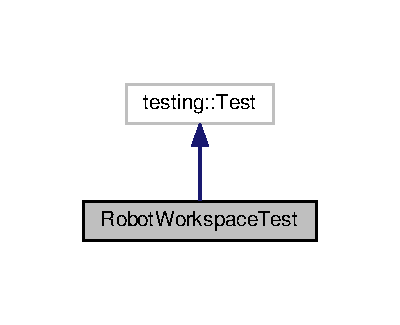
\includegraphics[width=192pt]{structRobotWorkspaceTest__inherit__graph}
\end{center}
\end{figure}


Collaboration diagram for Robot\+Workspace\+Test\+:\nopagebreak
\begin{figure}[H]
\begin{center}
\leavevmode
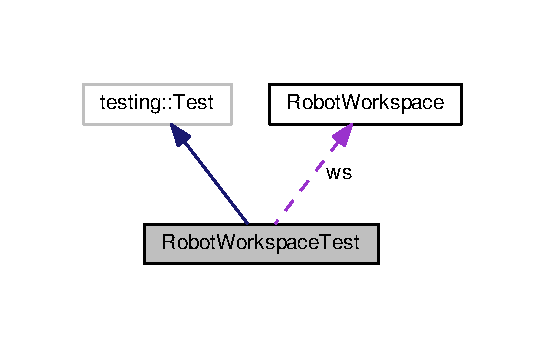
\includegraphics[width=262pt]{structRobotWorkspaceTest__coll__graph}
\end{center}
\end{figure}
\subsection*{Public Member Functions}
\begin{DoxyCompactItemize}
\item 
void \hyperlink{structRobotWorkspaceTest_a2139bb8873c63aacf5096b299a639d96}{Set\+Up} ()
\item 
void \hyperlink{structRobotWorkspaceTest_a59c52221366f68ed23bd7db4a8c2925c}{Tear\+Down} ()
\end{DoxyCompactItemize}
\subsection*{Public Attributes}
\begin{DoxyCompactItemize}
\item 
\hyperlink{classRobotWorkspace}{Robot\+Workspace} $\ast$ \hyperlink{structRobotWorkspaceTest_a73b830760a8bdd06651032ec7adf83e9}{ws}
\end{DoxyCompactItemize}


\subsection{Detailed Description}
\hyperlink{classRobotWorkspace}{Robot\+Workspace} class test fixture. 

\subsection{Member Function Documentation}
\index{Robot\+Workspace\+Test@{Robot\+Workspace\+Test}!Set\+Up@{Set\+Up}}
\index{Set\+Up@{Set\+Up}!Robot\+Workspace\+Test@{Robot\+Workspace\+Test}}
\subsubsection[{\texorpdfstring{Set\+Up()}{SetUp()}}]{\setlength{\rightskip}{0pt plus 5cm}void Robot\+Workspace\+Test\+::\+Set\+Up (
\begin{DoxyParamCaption}
{}
\end{DoxyParamCaption}
)\hspace{0.3cm}{\ttfamily [inline]}}\hypertarget{structRobotWorkspaceTest_a2139bb8873c63aacf5096b299a639d96}{}\label{structRobotWorkspaceTest_a2139bb8873c63aacf5096b299a639d96}
\index{Robot\+Workspace\+Test@{Robot\+Workspace\+Test}!Tear\+Down@{Tear\+Down}}
\index{Tear\+Down@{Tear\+Down}!Robot\+Workspace\+Test@{Robot\+Workspace\+Test}}
\subsubsection[{\texorpdfstring{Tear\+Down()}{TearDown()}}]{\setlength{\rightskip}{0pt plus 5cm}void Robot\+Workspace\+Test\+::\+Tear\+Down (
\begin{DoxyParamCaption}
{}
\end{DoxyParamCaption}
)\hspace{0.3cm}{\ttfamily [inline]}}\hypertarget{structRobotWorkspaceTest_a59c52221366f68ed23bd7db4a8c2925c}{}\label{structRobotWorkspaceTest_a59c52221366f68ed23bd7db4a8c2925c}


\subsection{Member Data Documentation}
\index{Robot\+Workspace\+Test@{Robot\+Workspace\+Test}!ws@{ws}}
\index{ws@{ws}!Robot\+Workspace\+Test@{Robot\+Workspace\+Test}}
\subsubsection[{\texorpdfstring{ws}{ws}}]{\setlength{\rightskip}{0pt plus 5cm}{\bf Robot\+Workspace}$\ast$ Robot\+Workspace\+Test\+::ws}\hypertarget{structRobotWorkspaceTest_a73b830760a8bdd06651032ec7adf83e9}{}\label{structRobotWorkspaceTest_a73b830760a8bdd06651032ec7adf83e9}


The documentation for this struct was generated from the following file\+:\begin{DoxyCompactItemize}
\item 
/home/bala/workspace/\+Midterm project/\+C\+P\+P-\/\+R\+R\+T/test/\hyperlink{RobotWorkspaceTest_8cpp}{Robot\+Workspace\+Test.\+cpp}\end{DoxyCompactItemize}

\hypertarget{classRRT}{}\section{R\+RT Class Reference}
\label{classRRT}\index{R\+RT@{R\+RT}}


Class finds path.  




{\ttfamily \#include $<$R\+R\+T.\+h$>$}

\subsection*{Public Member Functions}
\begin{DoxyCompactItemize}
\item 
bool \hyperlink{classRRT_a536e56c03eaf1249701915a6d349d020}{is\+Goal} ()
\begin{DoxyCompactList}\small\item\em Checks if a point is goal point of robot. \end{DoxyCompactList}\item 
void \hyperlink{classRRT_ae4efbc3892eb9dfcb642d28d5a19c7e3}{sample\+From\+Cs} ()
\begin{DoxyCompactList}\small\item\em Find a random unvisited sample point from configuration space. \end{DoxyCompactList}\item 
void \hyperlink{classRRT_ab6c1cd83695cb7dc377ca450d63a60d3}{add\+To\+Tree} ()
\begin{DoxyCompactList}\small\item\em Add point details to tree. \end{DoxyCompactList}\item 
int \hyperlink{classRRT_aa66da1beaa73a2207673f8dcd5de5289}{compute\+New\+Point} ()
\begin{DoxyCompactList}\small\item\em Find a new \mbox{[}point nearest to random chosen point. \end{DoxyCompactList}\item 
bool \hyperlink{classRRT_a632b8a8b4de79fc73b9183bacdc0d350}{update\+Sample\+Space} ()
\begin{DoxyCompactList}\small\item\em Update sample space to remove the visited point. \end{DoxyCompactList}\item 
std\+::vector$<$ \hyperlink{structpoint}{point} $>$ \hyperlink{classRRT_a520e20c364793c033b1bb899d687967c}{build\+Path} ()
\begin{DoxyCompactList}\small\item\em Compute and build path form start to goal point. \end{DoxyCompactList}\item 
\hyperlink{classRRT_a0a7bb3a3af2d70c656764fbe8f6ae671}{R\+RT} ()
\begin{DoxyCompactList}\small\item\em Constructor to initialize all variables. \end{DoxyCompactList}\item 
virtual \hyperlink{classRRT_ab16d13c231d664dddaf41f904d5770f8}{$\sim$\+R\+RT} ()
\begin{DoxyCompactList}\small\item\em Gets arena boundary from user and stores the values. \end{DoxyCompactList}\end{DoxyCompactItemize}
\subsection*{Public Attributes}
\begin{DoxyCompactItemize}
\item 
std\+::shared\+\_\+ptr$<$ \hyperlink{classInputMap}{Input\+Map} $>$ \hyperlink{classRRT_a072ade92010a498a1a5158fcef0d9ee9}{Map}
\item 
int \hyperlink{classRRT_a85de597c47f635ac1804a7e2c98f717b}{start\+Point} \mbox{[}2\mbox{]}
\item 
int \hyperlink{classRRT_acdc27db3967b542df1ebab8da270bd72}{goal\+Point} \mbox{[}2\mbox{]}
\item 
int \hyperlink{classRRT_a319220aada572c19cbbd2cfe0eb99c6d}{sampled\+Point} \mbox{[}2\mbox{]}
\item 
int \hyperlink{classRRT_a86bebb284bab72fab29824d75f5cb5a1}{new\+Point} \mbox{[}2\mbox{]}
\item 
int \hyperlink{classRRT_a93596f78ae0f49d4f54c61ec5b50c2f8}{parent\+Point\+Index}
\item 
std\+::vector$<$ std\+::array$<$ int, 4 $>$ $>$ \hyperlink{classRRT_a6ac6f3ad0727baaa8a17a2ee64e5bd2b}{Tree}
\end{DoxyCompactItemize}


\subsection{Detailed Description}
Class finds path. 

This class finds path from start point to end point using \hyperlink{classRRT}{R\+RT} algorithm 

\subsection{Constructor \& Destructor Documentation}
\index{R\+RT@{R\+RT}!R\+RT@{R\+RT}}
\index{R\+RT@{R\+RT}!R\+RT@{R\+RT}}
\subsubsection[{\texorpdfstring{R\+R\+T()}{RRT()}}]{\setlength{\rightskip}{0pt plus 5cm}R\+R\+T\+::\+R\+RT (
\begin{DoxyParamCaption}
{}
\end{DoxyParamCaption}
)}\hypertarget{classRRT_a0a7bb3a3af2d70c656764fbe8f6ae671}{}\label{classRRT_a0a7bb3a3af2d70c656764fbe8f6ae671}


Constructor to initialize all variables. 


\begin{DoxyParams}{Parameters}
{\em None} & \\
\hline
\end{DoxyParams}
\begin{DoxyReturn}{Returns}
None 
\end{DoxyReturn}
\index{R\+RT@{R\+RT}!````~R\+RT@{$\sim$\+R\+RT}}
\index{````~R\+RT@{$\sim$\+R\+RT}!R\+RT@{R\+RT}}
\subsubsection[{\texorpdfstring{$\sim$\+R\+R\+T()}{~RRT()}}]{\setlength{\rightskip}{0pt plus 5cm}R\+R\+T\+::$\sim$\+R\+RT (
\begin{DoxyParamCaption}
{}
\end{DoxyParamCaption}
)\hspace{0.3cm}{\ttfamily [virtual]}}\hypertarget{classRRT_ab16d13c231d664dddaf41f904d5770f8}{}\label{classRRT_ab16d13c231d664dddaf41f904d5770f8}


Gets arena boundary from user and stores the values. 


\begin{DoxyParams}{Parameters}
{\em Input} & and output stream references \\
\hline
\end{DoxyParams}
\begin{DoxyReturn}{Returns}
None 
\end{DoxyReturn}


\subsection{Member Function Documentation}
\index{R\+RT@{R\+RT}!add\+To\+Tree@{add\+To\+Tree}}
\index{add\+To\+Tree@{add\+To\+Tree}!R\+RT@{R\+RT}}
\subsubsection[{\texorpdfstring{add\+To\+Tree()}{addToTree()}}]{\setlength{\rightskip}{0pt plus 5cm}void R\+R\+T\+::add\+To\+Tree (
\begin{DoxyParamCaption}
{}
\end{DoxyParamCaption}
)}\hypertarget{classRRT_ab6c1cd83695cb7dc377ca450d63a60d3}{}\label{classRRT_ab6c1cd83695cb7dc377ca450d63a60d3}


Add point details to tree. 


\begin{DoxyParams}{Parameters}
{\em None} & \\
\hline
\end{DoxyParams}
\begin{DoxyReturn}{Returns}
None 
\end{DoxyReturn}
\index{R\+RT@{R\+RT}!build\+Path@{build\+Path}}
\index{build\+Path@{build\+Path}!R\+RT@{R\+RT}}
\subsubsection[{\texorpdfstring{build\+Path()}{buildPath()}}]{\setlength{\rightskip}{0pt plus 5cm}std\+::vector$<$ {\bf point} $>$ R\+R\+T\+::build\+Path (
\begin{DoxyParamCaption}
{}
\end{DoxyParamCaption}
)}\hypertarget{classRRT_a520e20c364793c033b1bb899d687967c}{}\label{classRRT_a520e20c364793c033b1bb899d687967c}


Compute and build path form start to goal point. 


\begin{DoxyParams}{Parameters}
{\em None} & \\
\hline
\end{DoxyParams}
\begin{DoxyReturn}{Returns}
Vector containing points on path 
\end{DoxyReturn}
\index{R\+RT@{R\+RT}!compute\+New\+Point@{compute\+New\+Point}}
\index{compute\+New\+Point@{compute\+New\+Point}!R\+RT@{R\+RT}}
\subsubsection[{\texorpdfstring{compute\+New\+Point()}{computeNewPoint()}}]{\setlength{\rightskip}{0pt plus 5cm}int R\+R\+T\+::compute\+New\+Point (
\begin{DoxyParamCaption}
{}
\end{DoxyParamCaption}
)}\hypertarget{classRRT_aa66da1beaa73a2207673f8dcd5de5289}{}\label{classRRT_aa66da1beaa73a2207673f8dcd5de5289}


Find a new \mbox{[}point nearest to random chosen point. 


\begin{DoxyParams}{Parameters}
{\em None} & \\
\hline
\end{DoxyParams}
\begin{DoxyReturn}{Returns}
Integer representing index if the point iin tree 
\end{DoxyReturn}
\index{R\+RT@{R\+RT}!is\+Goal@{is\+Goal}}
\index{is\+Goal@{is\+Goal}!R\+RT@{R\+RT}}
\subsubsection[{\texorpdfstring{is\+Goal()}{isGoal()}}]{\setlength{\rightskip}{0pt plus 5cm}bool R\+R\+T\+::is\+Goal (
\begin{DoxyParamCaption}
{}
\end{DoxyParamCaption}
)}\hypertarget{classRRT_a536e56c03eaf1249701915a6d349d020}{}\label{classRRT_a536e56c03eaf1249701915a6d349d020}


Checks if a point is goal point of robot. 


\begin{DoxyParams}{Parameters}
{\em None} & \\
\hline
\end{DoxyParams}
\begin{DoxyReturn}{Returns}
True or False depending on the result 
\end{DoxyReturn}
\index{R\+RT@{R\+RT}!sample\+From\+Cs@{sample\+From\+Cs}}
\index{sample\+From\+Cs@{sample\+From\+Cs}!R\+RT@{R\+RT}}
\subsubsection[{\texorpdfstring{sample\+From\+Cs()}{sampleFromCs()}}]{\setlength{\rightskip}{0pt plus 5cm}void R\+R\+T\+::sample\+From\+Cs (
\begin{DoxyParamCaption}
{}
\end{DoxyParamCaption}
)}\hypertarget{classRRT_ae4efbc3892eb9dfcb642d28d5a19c7e3}{}\label{classRRT_ae4efbc3892eb9dfcb642d28d5a19c7e3}


Find a random unvisited sample point from configuration space. 


\begin{DoxyParams}{Parameters}
{\em None} & \\
\hline
\end{DoxyParams}
\begin{DoxyReturn}{Returns}
None 
\end{DoxyReturn}
\index{R\+RT@{R\+RT}!update\+Sample\+Space@{update\+Sample\+Space}}
\index{update\+Sample\+Space@{update\+Sample\+Space}!R\+RT@{R\+RT}}
\subsubsection[{\texorpdfstring{update\+Sample\+Space()}{updateSampleSpace()}}]{\setlength{\rightskip}{0pt plus 5cm}bool R\+R\+T\+::update\+Sample\+Space (
\begin{DoxyParamCaption}
{}
\end{DoxyParamCaption}
)}\hypertarget{classRRT_a632b8a8b4de79fc73b9183bacdc0d350}{}\label{classRRT_a632b8a8b4de79fc73b9183bacdc0d350}


Update sample space to remove the visited point. 


\begin{DoxyParams}{Parameters}
{\em None} & \\
\hline
\end{DoxyParams}
\begin{DoxyReturn}{Returns}
True or False depending on whether there is more points to visit or not 
\end{DoxyReturn}


\subsection{Member Data Documentation}
\index{R\+RT@{R\+RT}!goal\+Point@{goal\+Point}}
\index{goal\+Point@{goal\+Point}!R\+RT@{R\+RT}}
\subsubsection[{\texorpdfstring{goal\+Point}{goalPoint}}]{\setlength{\rightskip}{0pt plus 5cm}int R\+R\+T\+::goal\+Point\mbox{[}2\mbox{]}}\hypertarget{classRRT_acdc27db3967b542df1ebab8da270bd72}{}\label{classRRT_acdc27db3967b542df1ebab8da270bd72}
\index{R\+RT@{R\+RT}!Map@{Map}}
\index{Map@{Map}!R\+RT@{R\+RT}}
\subsubsection[{\texorpdfstring{Map}{Map}}]{\setlength{\rightskip}{0pt plus 5cm}std\+::shared\+\_\+ptr$<${\bf Input\+Map}$>$ R\+R\+T\+::\+Map}\hypertarget{classRRT_a072ade92010a498a1a5158fcef0d9ee9}{}\label{classRRT_a072ade92010a498a1a5158fcef0d9ee9}
\index{R\+RT@{R\+RT}!new\+Point@{new\+Point}}
\index{new\+Point@{new\+Point}!R\+RT@{R\+RT}}
\subsubsection[{\texorpdfstring{new\+Point}{newPoint}}]{\setlength{\rightskip}{0pt plus 5cm}int R\+R\+T\+::new\+Point\mbox{[}2\mbox{]}}\hypertarget{classRRT_a86bebb284bab72fab29824d75f5cb5a1}{}\label{classRRT_a86bebb284bab72fab29824d75f5cb5a1}
\index{R\+RT@{R\+RT}!parent\+Point\+Index@{parent\+Point\+Index}}
\index{parent\+Point\+Index@{parent\+Point\+Index}!R\+RT@{R\+RT}}
\subsubsection[{\texorpdfstring{parent\+Point\+Index}{parentPointIndex}}]{\setlength{\rightskip}{0pt plus 5cm}int R\+R\+T\+::parent\+Point\+Index}\hypertarget{classRRT_a93596f78ae0f49d4f54c61ec5b50c2f8}{}\label{classRRT_a93596f78ae0f49d4f54c61ec5b50c2f8}
\index{R\+RT@{R\+RT}!sampled\+Point@{sampled\+Point}}
\index{sampled\+Point@{sampled\+Point}!R\+RT@{R\+RT}}
\subsubsection[{\texorpdfstring{sampled\+Point}{sampledPoint}}]{\setlength{\rightskip}{0pt plus 5cm}int R\+R\+T\+::sampled\+Point\mbox{[}2\mbox{]}}\hypertarget{classRRT_a319220aada572c19cbbd2cfe0eb99c6d}{}\label{classRRT_a319220aada572c19cbbd2cfe0eb99c6d}
\index{R\+RT@{R\+RT}!start\+Point@{start\+Point}}
\index{start\+Point@{start\+Point}!R\+RT@{R\+RT}}
\subsubsection[{\texorpdfstring{start\+Point}{startPoint}}]{\setlength{\rightskip}{0pt plus 5cm}int R\+R\+T\+::start\+Point\mbox{[}2\mbox{]}}\hypertarget{classRRT_a85de597c47f635ac1804a7e2c98f717b}{}\label{classRRT_a85de597c47f635ac1804a7e2c98f717b}
\index{R\+RT@{R\+RT}!Tree@{Tree}}
\index{Tree@{Tree}!R\+RT@{R\+RT}}
\subsubsection[{\texorpdfstring{Tree}{Tree}}]{\setlength{\rightskip}{0pt plus 5cm}std\+::vector$<$std\+::array$<$int, 4$>$ $>$ R\+R\+T\+::\+Tree}\hypertarget{classRRT_a6ac6f3ad0727baaa8a17a2ee64e5bd2b}{}\label{classRRT_a6ac6f3ad0727baaa8a17a2ee64e5bd2b}


The documentation for this class was generated from the following files\+:\begin{DoxyCompactItemize}
\item 
/home/bala/workspace/\+Midterm project/\+C\+P\+P-\/\+R\+R\+T/include/\hyperlink{RRT_8h}{R\+R\+T.\+h}\item 
/home/bala/workspace/\+Midterm project/\+C\+P\+P-\/\+R\+R\+T/app/\hyperlink{RRT_8cpp}{R\+R\+T.\+cpp}\end{DoxyCompactItemize}

\hypertarget{classSquare}{}\section{Square Class Reference}
\label{classSquare}\index{Square@{Square}}


\hyperlink{classSquare}{Square} class that holds functions of \hyperlink{classSquare}{Square} obstacle.  




{\ttfamily \#include $<$Square.\+h$>$}



Inheritance diagram for Square\+:
\nopagebreak
\begin{figure}[H]
\begin{center}
\leavevmode
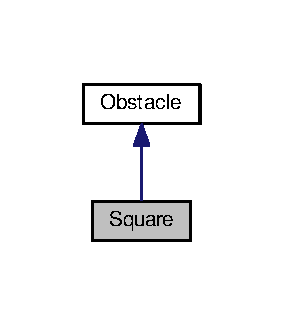
\includegraphics[width=136pt]{classSquare__inherit__graph}
\end{center}
\end{figure}


Collaboration diagram for Square\+:
\nopagebreak
\begin{figure}[H]
\begin{center}
\leavevmode
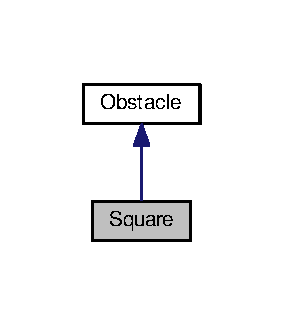
\includegraphics[width=136pt]{classSquare__coll__graph}
\end{center}
\end{figure}
\subsection*{Public Member Functions}
\begin{DoxyCompactItemize}
\item 
\hyperlink{classSquare_a3dc7ff9aefc2725172b5d3153973d243}{Square} ()
\begin{DoxyCompactList}\small\item\em Constructor to initialize all variables for obstacle class. \end{DoxyCompactList}\item 
void \hyperlink{classSquare_a1979921c7ae05d518c4392e0d5b8c156}{set\+Boundary} (std\+::istream \&in, std\+::ostream \&out)
\begin{DoxyCompactList}\small\item\em Gets boundary of square obstacle form user and updates the object. \end{DoxyCompactList}\item 
void \hyperlink{classSquare_afb76b9979da299090aa92f7e02465843}{disp\+Boundary} (std\+::ostream \&out)
\begin{DoxyCompactList}\small\item\em Display the square obstacle boundary points to user that has given. \end{DoxyCompactList}\item 
bool \hyperlink{classSquare_aa07ba26ea5675fea6dc90b2172ab13dd}{in\+Obstacle} (int x\+Coord, int y\+Coord)
\begin{DoxyCompactList}\small\item\em Checks if the point is inside the circle obstacle. \end{DoxyCompactList}\item 
void \hyperlink{classSquare_a395dc9319c9609d810e3f22eddbdcc81}{fill\+Obstacle} (std\+::vector$<$ \hyperlink{structpoint}{point} $>$ \&ob\+Map)
\begin{DoxyCompactList}\small\item\em Finds all points in circle obstacle. \end{DoxyCompactList}\item 
virtual \hyperlink{classSquare_a90af7ce1060cff7b717ceddb333846b8}{$\sim$\+Square} ()
\begin{DoxyCompactList}\small\item\em Destructor to free up space once object goes out of scope. \end{DoxyCompactList}\end{DoxyCompactItemize}


\subsection{Detailed Description}
\hyperlink{classSquare}{Square} class that holds functions of \hyperlink{classSquare}{Square} obstacle. 

\subsection{Constructor \& Destructor Documentation}
\index{Square@{Square}!Square@{Square}}
\index{Square@{Square}!Square@{Square}}
\subsubsection[{\texorpdfstring{Square()}{Square()}}]{\setlength{\rightskip}{0pt plus 5cm}Square\+::\+Square (
\begin{DoxyParamCaption}
{}
\end{DoxyParamCaption}
)}\hypertarget{classSquare_a3dc7ff9aefc2725172b5d3153973d243}{}\label{classSquare_a3dc7ff9aefc2725172b5d3153973d243}


Constructor to initialize all variables for obstacle class. 


\begin{DoxyParams}{Parameters}
{\em None} & \\
\hline
\end{DoxyParams}
\begin{DoxyReturn}{Returns}
None 
\end{DoxyReturn}
\index{Square@{Square}!````~Square@{$\sim$\+Square}}
\index{````~Square@{$\sim$\+Square}!Square@{Square}}
\subsubsection[{\texorpdfstring{$\sim$\+Square()}{~Square()}}]{\setlength{\rightskip}{0pt plus 5cm}Square\+::$\sim$\+Square (
\begin{DoxyParamCaption}
{}
\end{DoxyParamCaption}
)\hspace{0.3cm}{\ttfamily [virtual]}}\hypertarget{classSquare_a90af7ce1060cff7b717ceddb333846b8}{}\label{classSquare_a90af7ce1060cff7b717ceddb333846b8}


Destructor to free up space once object goes out of scope. 


\begin{DoxyParams}{Parameters}
{\em None} & \\
\hline
\end{DoxyParams}
\begin{DoxyReturn}{Returns}
None 
\end{DoxyReturn}


\subsection{Member Function Documentation}
\index{Square@{Square}!disp\+Boundary@{disp\+Boundary}}
\index{disp\+Boundary@{disp\+Boundary}!Square@{Square}}
\subsubsection[{\texorpdfstring{disp\+Boundary(std\+::ostream \&out)}{dispBoundary(std::ostream &out)}}]{\setlength{\rightskip}{0pt plus 5cm}void Square\+::disp\+Boundary (
\begin{DoxyParamCaption}
\item[{std\+::ostream \&}]{out}
\end{DoxyParamCaption}
)\hspace{0.3cm}{\ttfamily [virtual]}}\hypertarget{classSquare_afb76b9979da299090aa92f7e02465843}{}\label{classSquare_afb76b9979da299090aa92f7e02465843}


Display the square obstacle boundary points to user that has given. 


\begin{DoxyParams}{Parameters}
{\em Output} & stream \\
\hline
\end{DoxyParams}
\begin{DoxyReturn}{Returns}
input stream 
\end{DoxyReturn}


Implements \hyperlink{classObstacle_aba2625490b7d32632d585198038d279a}{Obstacle}.

\index{Square@{Square}!fill\+Obstacle@{fill\+Obstacle}}
\index{fill\+Obstacle@{fill\+Obstacle}!Square@{Square}}
\subsubsection[{\texorpdfstring{fill\+Obstacle(std\+::vector$<$ point $>$ \&ob\+Map)}{fillObstacle(std::vector< point > &obMap)}}]{\setlength{\rightskip}{0pt plus 5cm}void Square\+::fill\+Obstacle (
\begin{DoxyParamCaption}
\item[{std\+::vector$<$ {\bf point} $>$ \&}]{ob\+Map}
\end{DoxyParamCaption}
)\hspace{0.3cm}{\ttfamily [virtual]}}\hypertarget{classSquare_a395dc9319c9609d810e3f22eddbdcc81}{}\label{classSquare_a395dc9319c9609d810e3f22eddbdcc81}


Finds all points in circle obstacle. 


\begin{DoxyParams}{Parameters}
{\em Vector} & to hold all points of obstacle \\
\hline
\end{DoxyParams}
\begin{DoxyReturn}{Returns}
None 
\end{DoxyReturn}


Implements \hyperlink{classObstacle_ade69ded6cb0d58ff914e64aaef4a0464}{Obstacle}.

\index{Square@{Square}!in\+Obstacle@{in\+Obstacle}}
\index{in\+Obstacle@{in\+Obstacle}!Square@{Square}}
\subsubsection[{\texorpdfstring{in\+Obstacle(int x\+Coord, int y\+Coord)}{inObstacle(int xCoord, int yCoord)}}]{\setlength{\rightskip}{0pt plus 5cm}bool Square\+::in\+Obstacle (
\begin{DoxyParamCaption}
\item[{int}]{x\+Coord, }
\item[{int}]{y\+Coord}
\end{DoxyParamCaption}
)\hspace{0.3cm}{\ttfamily [virtual]}}\hypertarget{classSquare_aa07ba26ea5675fea6dc90b2172ab13dd}{}\label{classSquare_aa07ba26ea5675fea6dc90b2172ab13dd}


Checks if the point is inside the circle obstacle. 


\begin{DoxyParams}{Parameters}
{\em X} & and y coordinates for the point to be checked \\
\hline
\end{DoxyParams}
\begin{DoxyReturn}{Returns}
True if the point is inside obstacle else false 
\end{DoxyReturn}


Implements \hyperlink{classObstacle_a52c373a98616f6c41058f725b73479f5}{Obstacle}.

\index{Square@{Square}!set\+Boundary@{set\+Boundary}}
\index{set\+Boundary@{set\+Boundary}!Square@{Square}}
\subsubsection[{\texorpdfstring{set\+Boundary(std\+::istream \&in, std\+::ostream \&out)}{setBoundary(std::istream &in, std::ostream &out)}}]{\setlength{\rightskip}{0pt plus 5cm}void Square\+::set\+Boundary (
\begin{DoxyParamCaption}
\item[{std\+::istream \&}]{in, }
\item[{std\+::ostream \&}]{out}
\end{DoxyParamCaption}
)\hspace{0.3cm}{\ttfamily [virtual]}}\hypertarget{classSquare_a1979921c7ae05d518c4392e0d5b8c156}{}\label{classSquare_a1979921c7ae05d518c4392e0d5b8c156}


Gets boundary of square obstacle form user and updates the object. 


\begin{DoxyParams}{Parameters}
{\em Input} & and output stream \\
\hline
\end{DoxyParams}
\begin{DoxyReturn}{Returns}
None 
\end{DoxyReturn}


Implements \hyperlink{classObstacle_a8915ad90dc24f48df3ff0c38e8c695aa}{Obstacle}.



The documentation for this class was generated from the following files\+:\begin{DoxyCompactItemize}
\item 
/home/bala/workspace/\+Midterm project/\+C\+P\+P-\/\+R\+R\+T/include/\hyperlink{Square_8h}{Square.\+h}\item 
/home/bala/workspace/\+Midterm project/\+C\+P\+P-\/\+R\+R\+T/app/\hyperlink{Square_8cpp}{Square.\+cpp}\end{DoxyCompactItemize}

\hypertarget{structSquareTest}{}\section{Square\+Test Struct Reference}
\label{structSquareTest}\index{Square\+Test@{Square\+Test}}


\hyperlink{classSquare}{Square} class test fixture.  




Inheritance diagram for Square\+Test\+:\nopagebreak
\begin{figure}[H]
\begin{center}
\leavevmode
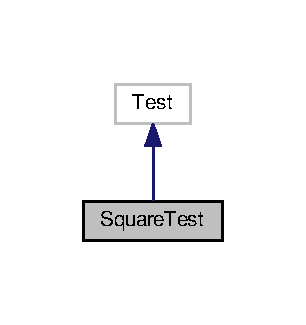
\includegraphics[width=147pt]{structSquareTest__inherit__graph}
\end{center}
\end{figure}


Collaboration diagram for Square\+Test\+:\nopagebreak
\begin{figure}[H]
\begin{center}
\leavevmode
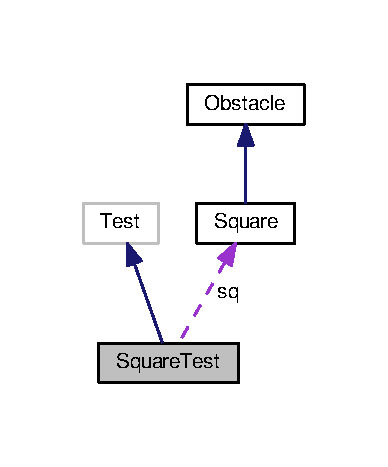
\includegraphics[width=186pt]{structSquareTest__coll__graph}
\end{center}
\end{figure}
\subsection*{Public Member Functions}
\begin{DoxyCompactItemize}
\item 
void \hyperlink{structSquareTest_ac719b65aeeaff1b1af8df1edff6f65d2}{Set\+Up} ()
\item 
void \hyperlink{structSquareTest_a30608c5d65d639a9957447218dcc997c}{Tear\+Down} ()
\end{DoxyCompactItemize}
\subsection*{Public Attributes}
\begin{DoxyCompactItemize}
\item 
\hyperlink{classSquare}{Square} $\ast$ \hyperlink{structSquareTest_a593accc2090fe5d6a462c416e712ff5a}{sq}
\end{DoxyCompactItemize}


\subsection{Detailed Description}
\hyperlink{classSquare}{Square} class test fixture. 

\subsection{Member Function Documentation}
\index{Square\+Test@{Square\+Test}!Set\+Up@{Set\+Up}}
\index{Set\+Up@{Set\+Up}!Square\+Test@{Square\+Test}}
\subsubsection[{\texorpdfstring{Set\+Up()}{SetUp()}}]{\setlength{\rightskip}{0pt plus 5cm}void Square\+Test\+::\+Set\+Up (
\begin{DoxyParamCaption}
{}
\end{DoxyParamCaption}
)\hspace{0.3cm}{\ttfamily [inline]}}\hypertarget{structSquareTest_ac719b65aeeaff1b1af8df1edff6f65d2}{}\label{structSquareTest_ac719b65aeeaff1b1af8df1edff6f65d2}
\index{Square\+Test@{Square\+Test}!Tear\+Down@{Tear\+Down}}
\index{Tear\+Down@{Tear\+Down}!Square\+Test@{Square\+Test}}
\subsubsection[{\texorpdfstring{Tear\+Down()}{TearDown()}}]{\setlength{\rightskip}{0pt plus 5cm}void Square\+Test\+::\+Tear\+Down (
\begin{DoxyParamCaption}
{}
\end{DoxyParamCaption}
)\hspace{0.3cm}{\ttfamily [inline]}}\hypertarget{structSquareTest_a30608c5d65d639a9957447218dcc997c}{}\label{structSquareTest_a30608c5d65d639a9957447218dcc997c}


\subsection{Member Data Documentation}
\index{Square\+Test@{Square\+Test}!sq@{sq}}
\index{sq@{sq}!Square\+Test@{Square\+Test}}
\subsubsection[{\texorpdfstring{sq}{sq}}]{\setlength{\rightskip}{0pt plus 5cm}{\bf Square}$\ast$ Square\+Test\+::sq}\hypertarget{structSquareTest_a593accc2090fe5d6a462c416e712ff5a}{}\label{structSquareTest_a593accc2090fe5d6a462c416e712ff5a}


The documentation for this struct was generated from the following file\+:\begin{DoxyCompactItemize}
\item 
/home/bala/workspace/\+Midterm project/\+C\+P\+P-\/\+R\+R\+T/test/\hyperlink{ObstacleTest_8cpp}{Obstacle\+Test.\+cpp}\end{DoxyCompactItemize}

\hypertarget{structStructure}{}\section{Structure Struct Reference}
\label{structStructure}\index{Structure@{Structure}}


\hyperlink{structStructure}{Structure} to hold x and y co-\/odinates of point. x and y co-\/odinates of point.  




\subsection{Detailed Description}
\hyperlink{structStructure}{Structure} to hold x and y co-\/odinates of point. x and y co-\/odinates of point. 

The documentation for this struct was generated from the following file\+:\begin{DoxyCompactItemize}
\item 
/home/bala/workspace/\+Midterm project/\+C\+P\+P-\/\+R\+R\+T/include/\hyperlink{Obstacle_8h}{Obstacle.\+h}\end{DoxyCompactItemize}

\chapter{File Documentation}
\hypertarget{Circle_8cpp}{}\section{/home/bala/workspace/\+Midterm project/\+C\+P\+P-\/\+R\+R\+T/app/\+Circle.cpp File Reference}
\label{Circle_8cpp}\index{/home/bala/workspace/\+Midterm project/\+C\+P\+P-\/\+R\+R\+T/app/\+Circle.\+cpp@{/home/bala/workspace/\+Midterm project/\+C\+P\+P-\/\+R\+R\+T/app/\+Circle.\+cpp}}
{\ttfamily \#include \char`\"{}../include/\+Circle.\+h\char`\"{}}\\*
Include dependency graph for Circle.\+cpp\+:\nopagebreak
\begin{figure}[H]
\begin{center}
\leavevmode
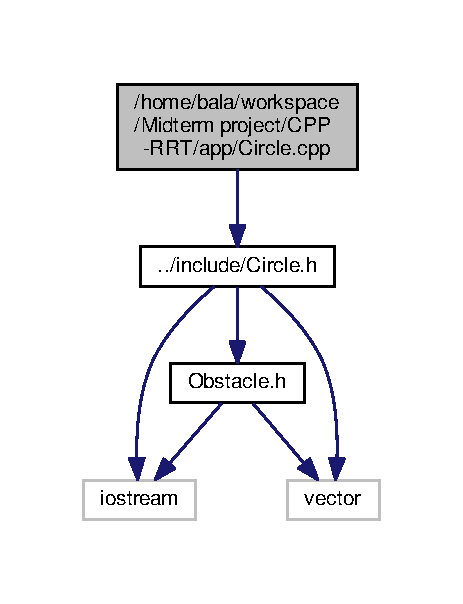
\includegraphics[width=222pt]{Circle_8cpp__incl}
\end{center}
\end{figure}

\hypertarget{app_2CMakeLists_8txt}{}\section{/home/bala/workspace/\+Midterm project/\+C\+P\+P-\/\+R\+R\+T/app/\+C\+Make\+Lists.txt File Reference}
\label{app_2CMakeLists_8txt}\index{/home/bala/workspace/\+Midterm project/\+C\+P\+P-\/\+R\+R\+T/app/\+C\+Make\+Lists.\+txt@{/home/bala/workspace/\+Midterm project/\+C\+P\+P-\/\+R\+R\+T/app/\+C\+Make\+Lists.\+txt}}
\subsection*{Functions}
\begin{DoxyCompactItemize}
\item 
\hyperlink{app_2CMakeLists_8txt_a7e958e3c8713aa5128ec051f4a183ac6}{add\+\_\+executable} (shell-\/app main.\+cpp Obstacle.\+cpp Square.\+cpp Circle.\+cpp Robot\+Workspace.\+cpp Input\+Map.\+cpp Path\+Display.\+cpp R\+R\+T.\+cpp) include\+\_\+directories(\$
\end{DoxyCompactItemize}


\subsection{Function Documentation}
\index{app/\+C\+Make\+Lists.\+txt@{app/\+C\+Make\+Lists.\+txt}!add\+\_\+executable@{add\+\_\+executable}}
\index{add\+\_\+executable@{add\+\_\+executable}!app/\+C\+Make\+Lists.\+txt@{app/\+C\+Make\+Lists.\+txt}}
\subsubsection[{\texorpdfstring{add\+\_\+executable(shell-\/app main.\+cpp Obstacle.\+cpp Square.\+cpp Circle.\+cpp Robot\+Workspace.\+cpp Input\+Map.\+cpp Path\+Display.\+cpp R\+R\+T.\+cpp) include\+\_\+directories(\$}{add_executable(shell-app main.cpp Obstacle.cpp Square.cpp Circle.cpp RobotWorkspace.cpp InputMap.cpp PathDisplay.cpp RRT.cpp) include_directories($}}]{\setlength{\rightskip}{0pt plus 5cm}add\+\_\+executable (
\begin{DoxyParamCaption}
\item[{shell-\/app main.\+cpp Obstacle.\+cpp Square.\+cpp Circle.\+cpp Robot\+Workspace.\+cpp Input\+Map.\+cpp Path\+Display.\+cpp R\+R\+T.}]{cpp}
\end{DoxyParamCaption}
)}\hypertarget{app_2CMakeLists_8txt_a7e958e3c8713aa5128ec051f4a183ac6}{}\label{app_2CMakeLists_8txt_a7e958e3c8713aa5128ec051f4a183ac6}

\hypertarget{test_2CMakeLists_8txt}{}\section{/home/bala/workspace/\+Midterm project/\+C\+P\+P-\/\+R\+R\+T/test/\+C\+Make\+Lists.txt File Reference}
\label{test_2CMakeLists_8txt}\index{/home/bala/workspace/\+Midterm project/\+C\+P\+P-\/\+R\+R\+T/test/\+C\+Make\+Lists.\+txt@{/home/bala/workspace/\+Midterm project/\+C\+P\+P-\/\+R\+R\+T/test/\+C\+Make\+Lists.\+txt}}
\subsection*{Functions}
\begin{DoxyCompactItemize}
\item 
\hyperlink{test_2CMakeLists_8txt_aa7d57915363f105030e3e5567ab252ad}{set} (G\+T\+E\+S\+T\+\_\+\+S\+H\+U\+F\+F\+LE 1) \hyperlink{app_2CMakeLists_8txt_a7e958e3c8713aa5128ec051f4a183ac6}{add\+\_\+executable}(cpp-\/test main.\+cpp Obstacle\+Test.\+cpp Robot\+Workspace\+Test.\+cpp Input\+Map\+Test.\+cpp Path\+Display\+Test.\+cpp R\+R\+T\+Test.\+cpp../app/Circle.\+cpp../app/Input\+Map.\+cpp../app/Obstacle.\+cpp../app/Path\+Display.\+cpp../app/Robot\+Workspace.\+cpp../app/R\+R\+T.\+cpp../app/Square.\+cpp) target\+\_\+include\+\_\+directories(cpp-\/test P\+U\+B\+L\+I\+C../vendor/googletest/googletest/include \$
\end{DoxyCompactItemize}


\subsection{Function Documentation}
\index{test/\+C\+Make\+Lists.\+txt@{test/\+C\+Make\+Lists.\+txt}!set@{set}}
\index{set@{set}!test/\+C\+Make\+Lists.\+txt@{test/\+C\+Make\+Lists.\+txt}}
\subsubsection[{\texorpdfstring{set(\+G\+T\+E\+S\+T\+\_\+\+S\+H\+U\+F\+F\+L\+E 1) add\+\_\+executable(cpp-\/test main.\+cpp Obstacle\+Test.\+cpp Robot\+Workspace\+Test.\+cpp Input\+Map\+Test.\+cpp Path\+Display\+Test.\+cpp R\+R\+T\+Test.\+cpp../app/\+Circle.\+cpp../app/\+Input\+Map.\+cpp../app/\+Obstacle.\+cpp../app/\+Path\+Display.\+cpp../app/\+Robot\+Workspace.\+cpp../app/\+R\+R\+T.\+cpp../app/\+Square.\+cpp) target\+\_\+include\+\_\+directories(cpp-\/test P\+U\+B\+L\+I\+C../vendor/googletest/googletest/include \$}{set(GTEST_SHUFFLE 1) add_executable(cpp-test main.cpp ObstacleTest.cpp RobotWorkspaceTest.cpp InputMapTest.cpp PathDisplayTest.cpp RRTTest.cpp../app/Circle.cpp../app/InputMap.cpp../app/Obstacle.cpp../app/PathDisplay.cpp../app/RobotWorkspace.cpp../app/RRT.cpp../app/Square.cpp) target_include_directories(cpp-test PUBLIC../vendor/googletest/googletest/include $}}]{\setlength{\rightskip}{0pt plus 5cm}set (
\begin{DoxyParamCaption}
\item[{G\+T\+E\+S\+T\+\_\+\+S\+H\+U\+F\+F\+LE}]{1}
\end{DoxyParamCaption}
)}\hypertarget{test_2CMakeLists_8txt_aa7d57915363f105030e3e5567ab252ad}{}\label{test_2CMakeLists_8txt_aa7d57915363f105030e3e5567ab252ad}

\hypertarget{InputMap_8cpp}{}\section{/home/bala/workspace/\+Midterm project/\+C\+P\+P-\/\+R\+R\+T/app/\+Input\+Map.cpp File Reference}
\label{InputMap_8cpp}\index{/home/bala/workspace/\+Midterm project/\+C\+P\+P-\/\+R\+R\+T/app/\+Input\+Map.\+cpp@{/home/bala/workspace/\+Midterm project/\+C\+P\+P-\/\+R\+R\+T/app/\+Input\+Map.\+cpp}}
{\ttfamily \#include $<$iostream$>$}\\*
{\ttfamily \#include \char`\"{}../include/\+Input\+Map.\+h\char`\"{}}\\*
Include dependency graph for Input\+Map.\+cpp\+:
\nopagebreak
\begin{figure}[H]
\begin{center}
\leavevmode
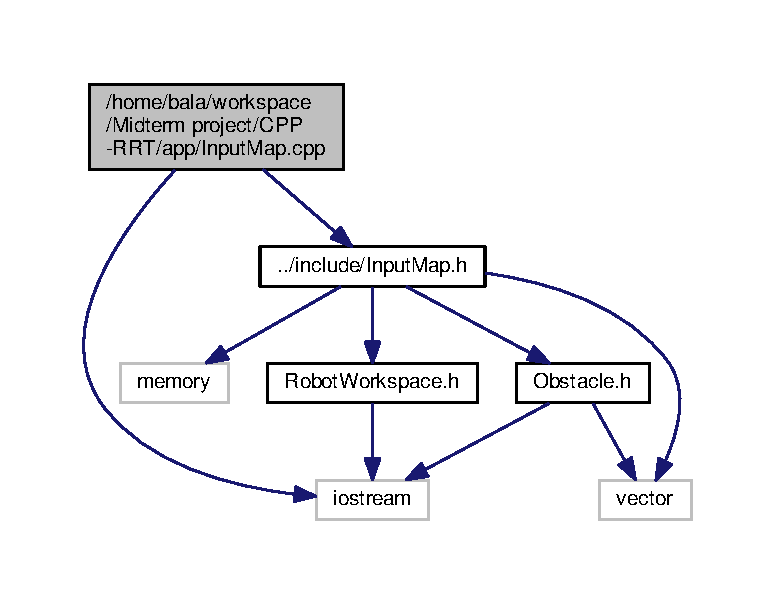
\includegraphics[width=350pt]{InputMap_8cpp__incl}
\end{center}
\end{figure}

\hypertarget{app_2main_8cpp}{}\section{/home/bala/workspace/\+Midterm project/\+C\+P\+P-\/\+R\+R\+T/app/main.cpp File Reference}
\label{app_2main_8cpp}\index{/home/bala/workspace/\+Midterm project/\+C\+P\+P-\/\+R\+R\+T/app/main.\+cpp@{/home/bala/workspace/\+Midterm project/\+C\+P\+P-\/\+R\+R\+T/app/main.\+cpp}}
{\ttfamily \#include $<$iostream$>$}\\*
{\ttfamily \#include $<$vector$>$}\\*
{\ttfamily \#include $<$memory$>$}\\*
{\ttfamily \#include $<$utility$>$}\\*
{\ttfamily \#include $<$sstream$>$}\\*
{\ttfamily \#include \char`\"{}../include/\+Input\+Map.\+h\char`\"{}}\\*
{\ttfamily \#include \char`\"{}../include/\+Robot\+Workspace.\+h\char`\"{}}\\*
{\ttfamily \#include \char`\"{}../include/\+Obstacle.\+h\char`\"{}}\\*
{\ttfamily \#include \char`\"{}../include/\+Square.\+h\char`\"{}}\\*
{\ttfamily \#include \char`\"{}../include/\+Circle.\+h\char`\"{}}\\*
{\ttfamily \#include \char`\"{}../include/\+Path\+Display.\+h\char`\"{}}\\*
{\ttfamily \#include \char`\"{}../include/\+R\+R\+T.\+h\char`\"{}}\\*
Include dependency graph for main.\+cpp\+:\nopagebreak
\begin{figure}[H]
\begin{center}
\leavevmode
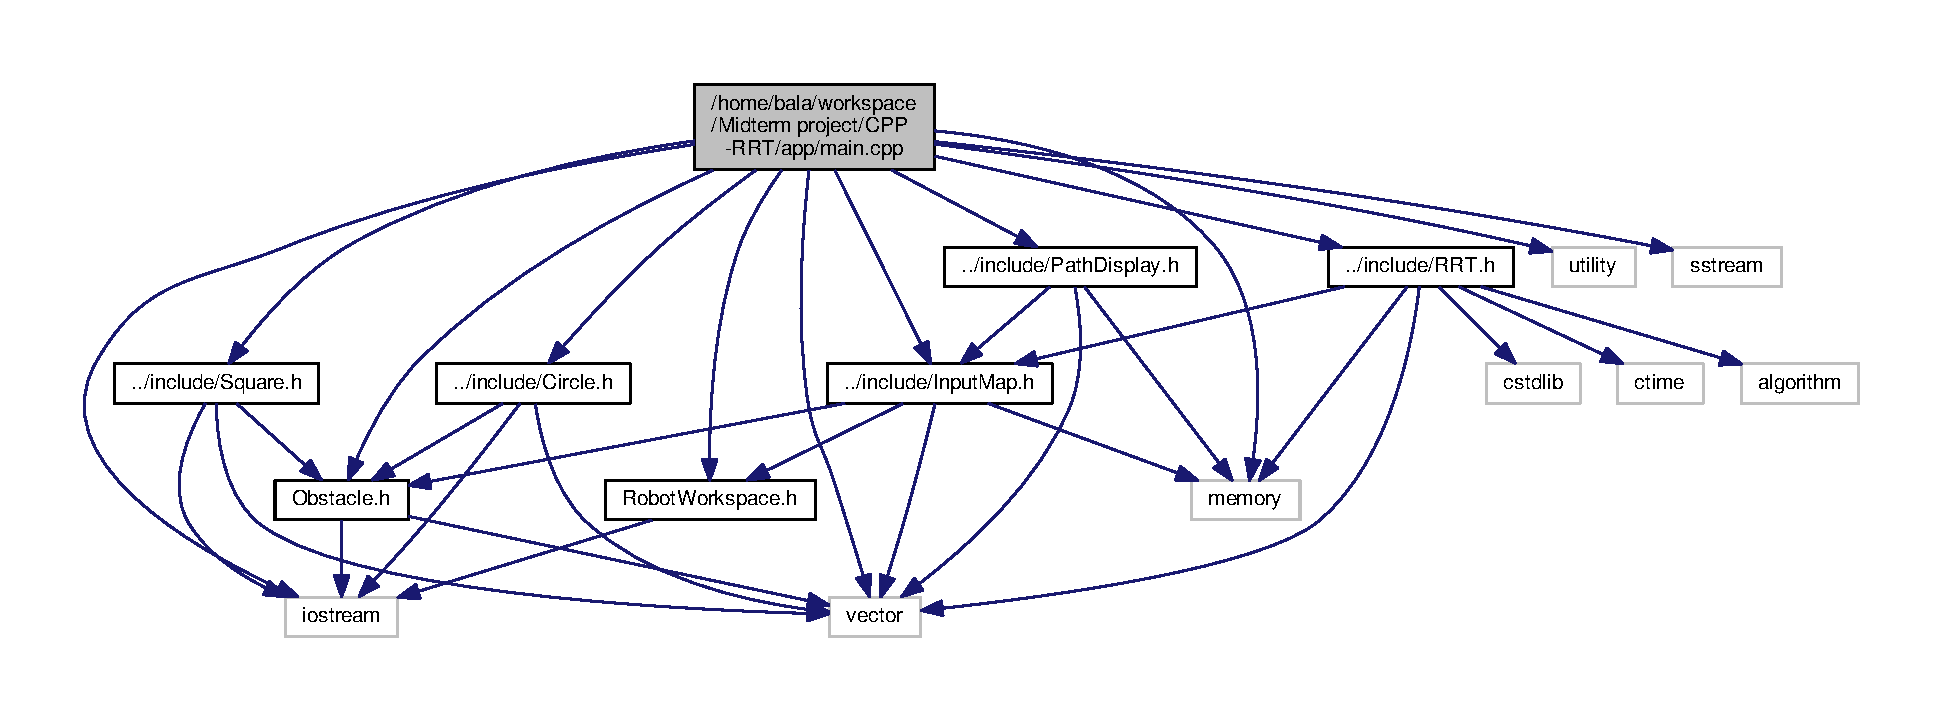
\includegraphics[width=350pt]{app_2main_8cpp__incl}
\end{center}
\end{figure}
\subsection*{Functions}
\begin{DoxyCompactItemize}
\item 
int \hyperlink{app_2main_8cpp_ae66f6b31b5ad750f1fe042a706a4e3d4}{main} ()
\begin{DoxyCompactList}\small\item\em Demo function to perform \hyperlink{classRRT}{R\+RT} path planning algorithm. \end{DoxyCompactList}\end{DoxyCompactItemize}


\subsection{Function Documentation}
\index{app/main.\+cpp@{app/main.\+cpp}!main@{main}}
\index{main@{main}!app/main.\+cpp@{app/main.\+cpp}}
\subsubsection[{\texorpdfstring{main()}{main()}}]{\setlength{\rightskip}{0pt plus 5cm}int main (
\begin{DoxyParamCaption}
{}
\end{DoxyParamCaption}
)}\hypertarget{app_2main_8cpp_ae66f6b31b5ad750f1fe042a706a4e3d4}{}\label{app_2main_8cpp_ae66f6b31b5ad750f1fe042a706a4e3d4}


Demo function to perform \hyperlink{classRRT}{R\+RT} path planning algorithm. 


\hypertarget{test_2main_8cpp}{}\section{/home/bala/workspace/\+Midterm project/\+C\+P\+P-\/\+R\+R\+T/test/main.cpp File Reference}
\label{test_2main_8cpp}\index{/home/bala/workspace/\+Midterm project/\+C\+P\+P-\/\+R\+R\+T/test/main.\+cpp@{/home/bala/workspace/\+Midterm project/\+C\+P\+P-\/\+R\+R\+T/test/main.\+cpp}}
{\ttfamily \#include $<$gtest/gtest.\+h$>$}\\*
Include dependency graph for main.\+cpp\+:\nopagebreak
\begin{figure}[H]
\begin{center}
\leavevmode
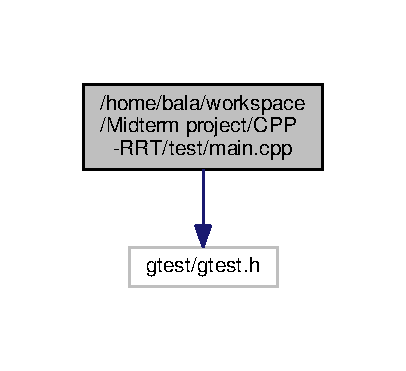
\includegraphics[width=195pt]{test_2main_8cpp__incl}
\end{center}
\end{figure}
\subsection*{Functions}
\begin{DoxyCompactItemize}
\item 
int \hyperlink{test_2main_8cpp_a3c04138a5bfe5d72780bb7e82a18e627}{main} (int argc, char $\ast$$\ast$argv)
\end{DoxyCompactItemize}


\subsection{Function Documentation}
\index{test/main.\+cpp@{test/main.\+cpp}!main@{main}}
\index{main@{main}!test/main.\+cpp@{test/main.\+cpp}}
\subsubsection[{\texorpdfstring{main(int argc, char $\ast$$\ast$argv)}{main(int argc, char **argv)}}]{\setlength{\rightskip}{0pt plus 5cm}int main (
\begin{DoxyParamCaption}
\item[{int}]{argc, }
\item[{char $\ast$$\ast$}]{argv}
\end{DoxyParamCaption}
)}\hypertarget{test_2main_8cpp_a3c04138a5bfe5d72780bb7e82a18e627}{}\label{test_2main_8cpp_a3c04138a5bfe5d72780bb7e82a18e627}

\hypertarget{Obstacle_8cpp}{}\section{/home/bala/workspace/\+Midterm project/\+C\+P\+P-\/\+R\+R\+T/app/\+Obstacle.cpp File Reference}
\label{Obstacle_8cpp}\index{/home/bala/workspace/\+Midterm project/\+C\+P\+P-\/\+R\+R\+T/app/\+Obstacle.\+cpp@{/home/bala/workspace/\+Midterm project/\+C\+P\+P-\/\+R\+R\+T/app/\+Obstacle.\+cpp}}
{\ttfamily \#include \char`\"{}../include/\+Obstacle.\+h\char`\"{}}\\*
Include dependency graph for Obstacle.\+cpp\+:\nopagebreak
\begin{figure}[H]
\begin{center}
\leavevmode
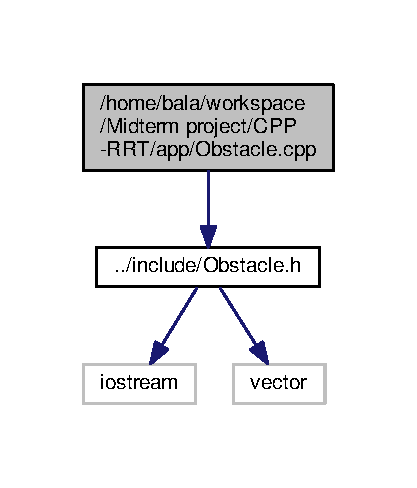
\includegraphics[width=200pt]{Obstacle_8cpp__incl}
\end{center}
\end{figure}

\hypertarget{PathDisplay_8cpp}{}\section{/home/bala/workspace/\+Midterm project/\+C\+P\+P-\/\+R\+R\+T/app/\+Path\+Display.cpp File Reference}
\label{PathDisplay_8cpp}\index{/home/bala/workspace/\+Midterm project/\+C\+P\+P-\/\+R\+R\+T/app/\+Path\+Display.\+cpp@{/home/bala/workspace/\+Midterm project/\+C\+P\+P-\/\+R\+R\+T/app/\+Path\+Display.\+cpp}}
{\ttfamily \#include $<$vector$>$}\\*
{\ttfamily \#include $<$iostream$>$}\\*
{\ttfamily \#include \char`\"{}../include/\+Path\+Display.\+h\char`\"{}}\\*
Include dependency graph for Path\+Display.\+cpp\+:
\nopagebreak
\begin{figure}[H]
\begin{center}
\leavevmode
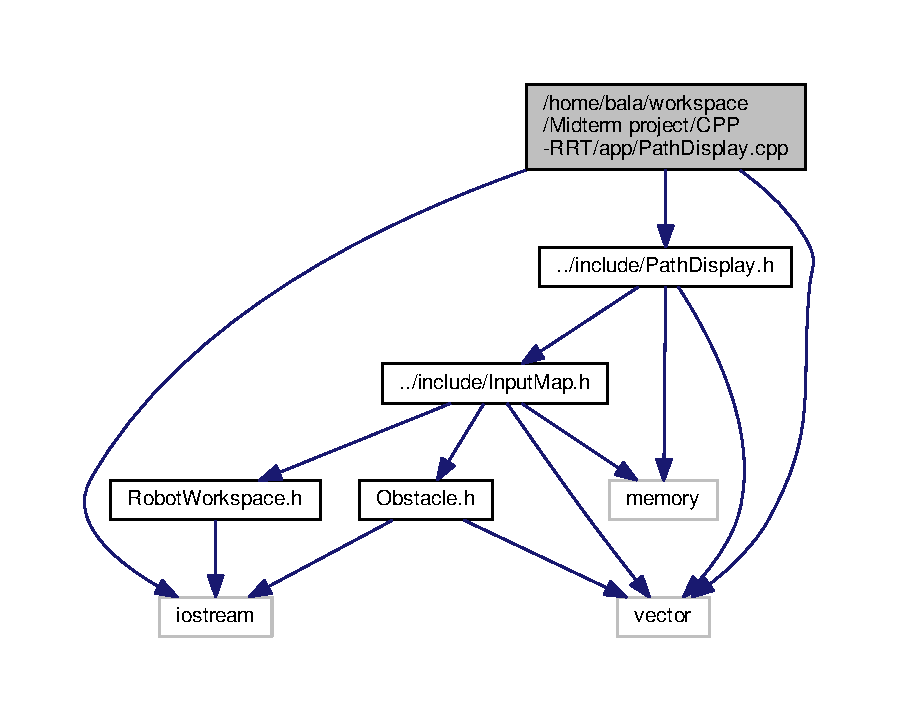
\includegraphics[width=350pt]{PathDisplay_8cpp__incl}
\end{center}
\end{figure}

\hypertarget{RobotWorkspace_8cpp}{}\section{/home/bala/workspace/\+Midterm project/\+C\+P\+P-\/\+R\+R\+T/app/\+Robot\+Workspace.cpp File Reference}
\label{RobotWorkspace_8cpp}\index{/home/bala/workspace/\+Midterm project/\+C\+P\+P-\/\+R\+R\+T/app/\+Robot\+Workspace.\+cpp@{/home/bala/workspace/\+Midterm project/\+C\+P\+P-\/\+R\+R\+T/app/\+Robot\+Workspace.\+cpp}}
{\ttfamily \#include \char`\"{}../include/\+Robot\+Workspace.\+h\char`\"{}}\\*
Include dependency graph for Robot\+Workspace.\+cpp\+:
\nopagebreak
\begin{figure}[H]
\begin{center}
\leavevmode
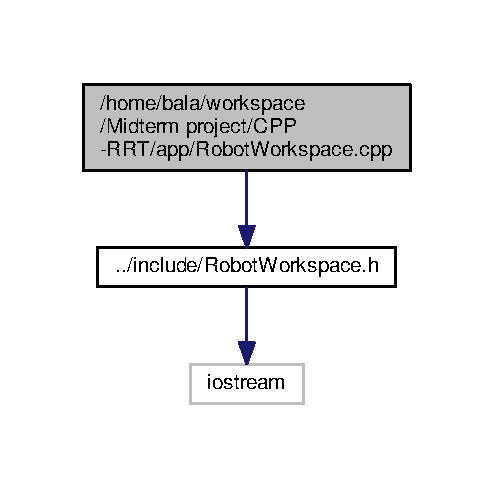
\includegraphics[width=237pt]{RobotWorkspace_8cpp__incl}
\end{center}
\end{figure}

\hypertarget{RRT_8cpp}{}\section{/home/bala/workspace/\+Midterm project/\+C\+P\+P-\/\+R\+R\+T/app/\+R\+RT.cpp File Reference}
\label{RRT_8cpp}\index{/home/bala/workspace/\+Midterm project/\+C\+P\+P-\/\+R\+R\+T/app/\+R\+R\+T.\+cpp@{/home/bala/workspace/\+Midterm project/\+C\+P\+P-\/\+R\+R\+T/app/\+R\+R\+T.\+cpp}}
{\ttfamily \#include \char`\"{}../include/\+R\+R\+T.\+h\char`\"{}}\\*
{\ttfamily \#include $<$vector$>$}\\*
{\ttfamily \#include $<$cstdlib$>$}\\*
{\ttfamily \#include $<$ctime$>$}\\*
{\ttfamily \#include $<$algorithm$>$}\\*
{\ttfamily \#include $<$cmath$>$}\\*
{\ttfamily \#include $<$iterator$>$}\\*
{\ttfamily \#include $<$utility$>$}\\*
{\ttfamily \#include $<$iostream$>$}\\*
Include dependency graph for R\+R\+T.\+cpp\+:\nopagebreak
\begin{figure}[H]
\begin{center}
\leavevmode
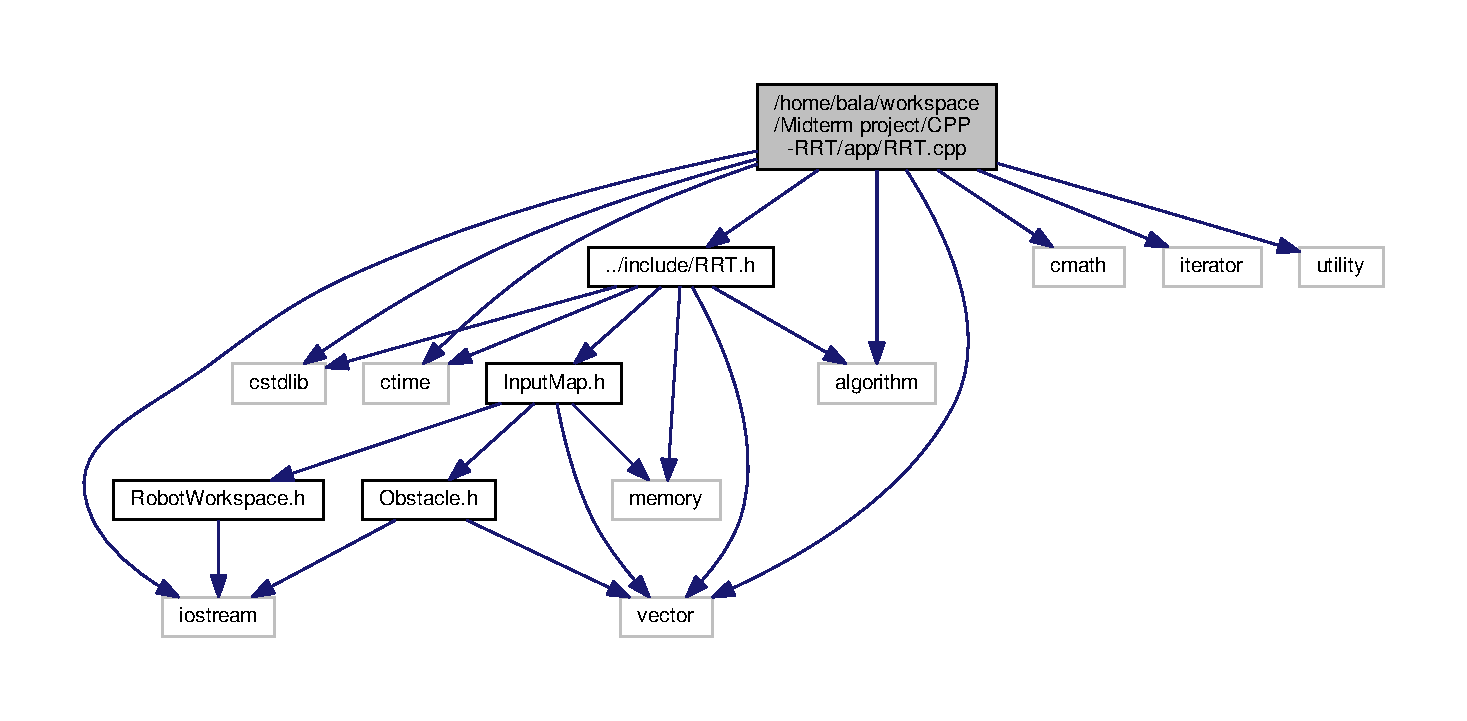
\includegraphics[width=350pt]{RRT_8cpp__incl}
\end{center}
\end{figure}

\hypertarget{Square_8cpp}{}\section{/home/bala/workspace/\+Midterm project/\+C\+P\+P-\/\+R\+R\+T/app/\+Square.cpp File Reference}
\label{Square_8cpp}\index{/home/bala/workspace/\+Midterm project/\+C\+P\+P-\/\+R\+R\+T/app/\+Square.\+cpp@{/home/bala/workspace/\+Midterm project/\+C\+P\+P-\/\+R\+R\+T/app/\+Square.\+cpp}}
{\ttfamily \#include \char`\"{}Square.\+h\char`\"{}}\\*
Include dependency graph for Square.\+cpp\+:
\nopagebreak
\begin{figure}[H]
\begin{center}
\leavevmode
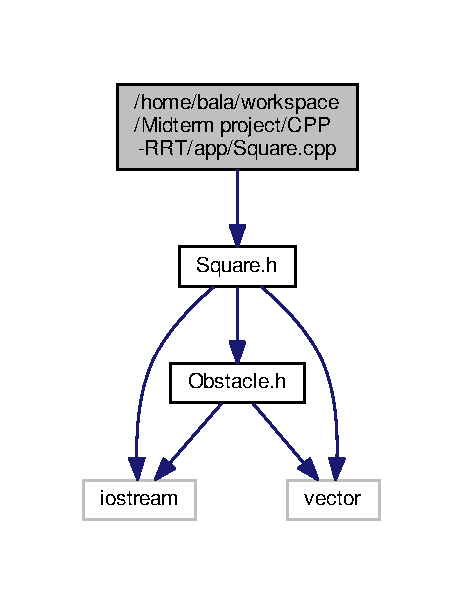
\includegraphics[width=222pt]{Square_8cpp__incl}
\end{center}
\end{figure}

\hypertarget{Circle_8h}{}\section{/home/bala/workspace/\+Midterm project/\+C\+P\+P-\/\+R\+R\+T/include/\+Circle.h File Reference}
\label{Circle_8h}\index{/home/bala/workspace/\+Midterm project/\+C\+P\+P-\/\+R\+R\+T/include/\+Circle.\+h@{/home/bala/workspace/\+Midterm project/\+C\+P\+P-\/\+R\+R\+T/include/\+Circle.\+h}}
{\ttfamily \#include $<$iostream$>$}\\*
{\ttfamily \#include $<$vector$>$}\\*
{\ttfamily \#include \char`\"{}Obstacle.\+h\char`\"{}}\\*
Include dependency graph for Circle.\+h\+:
\nopagebreak
\begin{figure}[H]
\begin{center}
\leavevmode
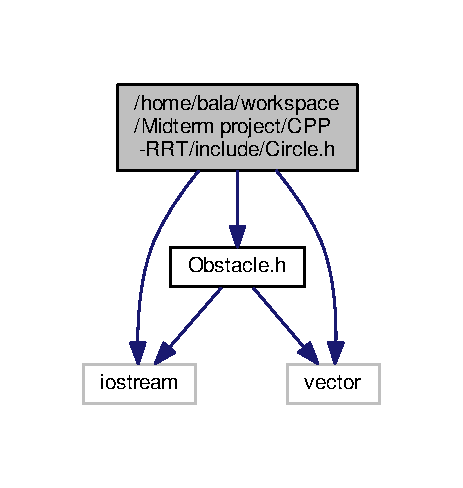
\includegraphics[width=222pt]{Circle_8h__incl}
\end{center}
\end{figure}
This graph shows which files directly or indirectly include this file\+:
\nopagebreak
\begin{figure}[H]
\begin{center}
\leavevmode
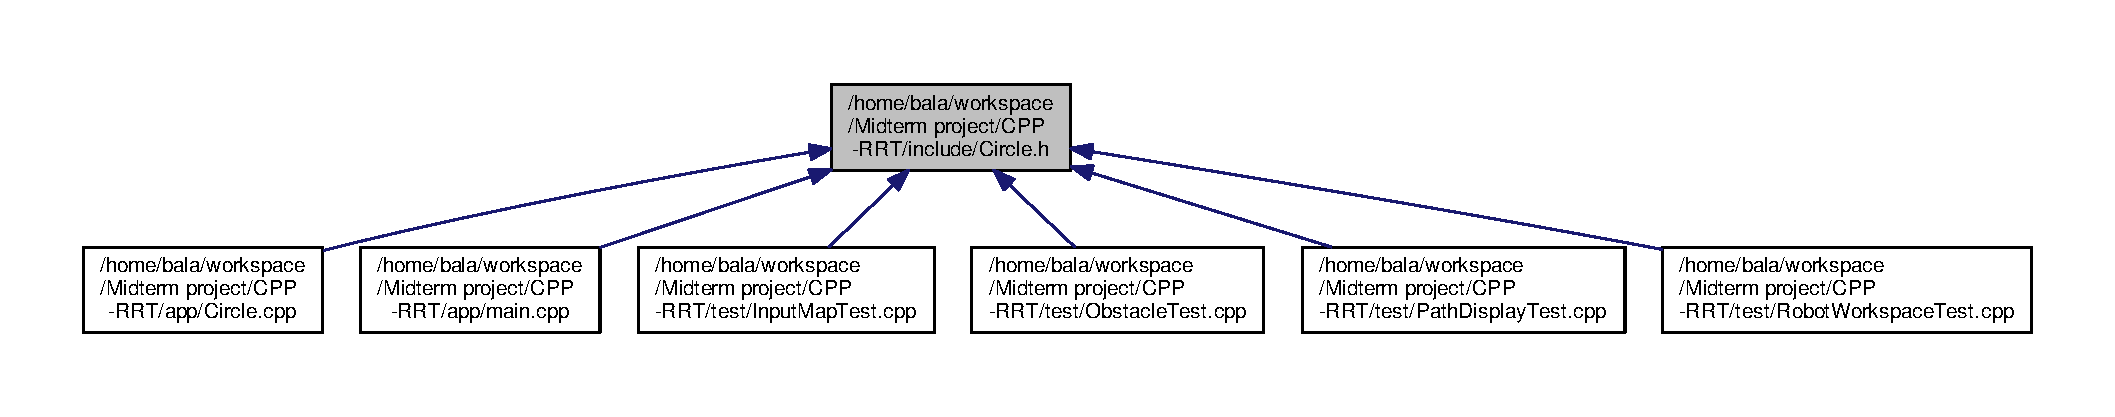
\includegraphics[width=350pt]{Circle_8h__dep__incl}
\end{center}
\end{figure}
\subsection*{Classes}
\begin{DoxyCompactItemize}
\item 
class \hyperlink{classCircle}{Circle}
\begin{DoxyCompactList}\small\item\em \hyperlink{classCircle}{Circle} class that holds functions of circular obstacle. \end{DoxyCompactList}\end{DoxyCompactItemize}

\hypertarget{InputMap_8h}{}\section{/home/bala/workspace/\+Midterm project/\+C\+P\+P-\/\+R\+R\+T/include/\+Input\+Map.h File Reference}
\label{InputMap_8h}\index{/home/bala/workspace/\+Midterm project/\+C\+P\+P-\/\+R\+R\+T/include/\+Input\+Map.\+h@{/home/bala/workspace/\+Midterm project/\+C\+P\+P-\/\+R\+R\+T/include/\+Input\+Map.\+h}}
{\ttfamily \#include $<$vector$>$}\\*
{\ttfamily \#include $<$memory$>$}\\*
{\ttfamily \#include \char`\"{}Obstacle.\+h\char`\"{}}\\*
{\ttfamily \#include \char`\"{}Robot\+Workspace.\+h\char`\"{}}\\*
Include dependency graph for Input\+Map.\+h\+:\nopagebreak
\begin{figure}[H]
\begin{center}
\leavevmode
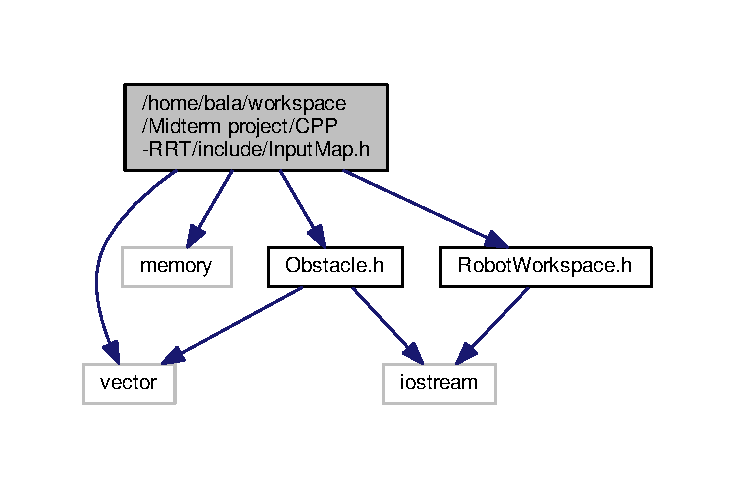
\includegraphics[width=350pt]{InputMap_8h__incl}
\end{center}
\end{figure}
This graph shows which files directly or indirectly include this file\+:\nopagebreak
\begin{figure}[H]
\begin{center}
\leavevmode
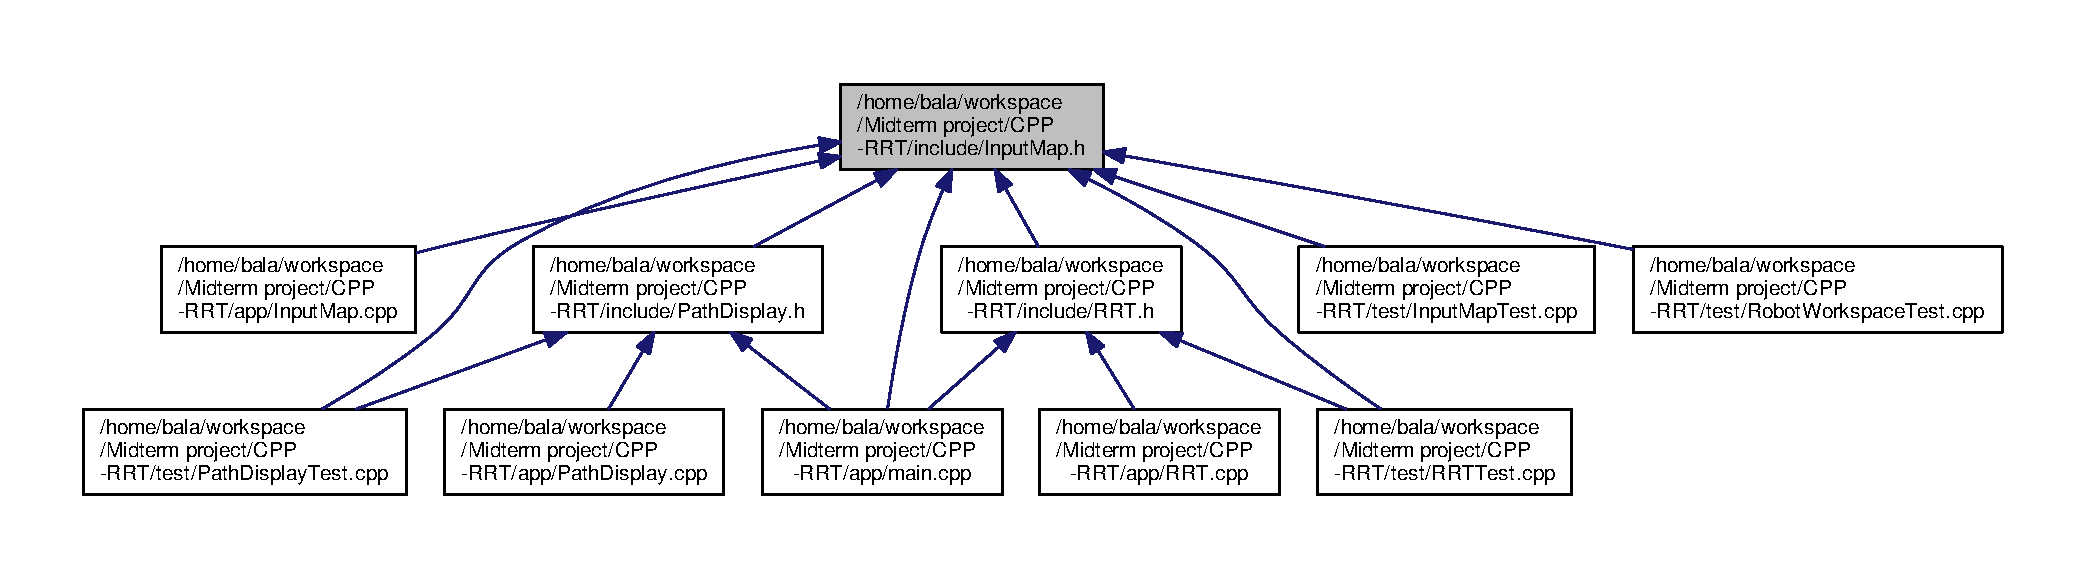
\includegraphics[width=350pt]{InputMap_8h__dep__incl}
\end{center}
\end{figure}
\subsection*{Classes}
\begin{DoxyCompactItemize}
\item 
class \hyperlink{classInputMap}{Input\+Map}
\begin{DoxyCompactList}\small\item\em Class holds map properties. \end{DoxyCompactList}\end{DoxyCompactItemize}

\hypertarget{lib_8hpp}{}\section{/home/bala/workspace/\+Midterm project/\+C\+P\+P-\/\+R\+R\+T/include/lib.hpp File Reference}
\label{lib_8hpp}\index{/home/bala/workspace/\+Midterm project/\+C\+P\+P-\/\+R\+R\+T/include/lib.\+hpp@{/home/bala/workspace/\+Midterm project/\+C\+P\+P-\/\+R\+R\+T/include/lib.\+hpp}}
{\ttfamily \#include $<$iostream$>$}\\*
Include dependency graph for lib.\+hpp\+:\nopagebreak
\begin{figure}[H]
\begin{center}
\leavevmode
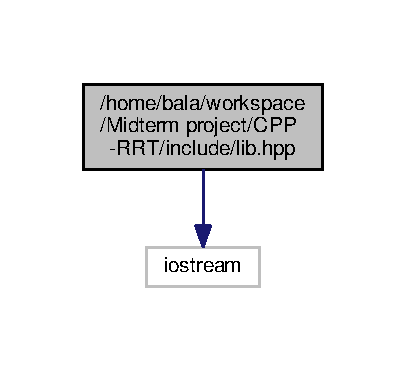
\includegraphics[width=195pt]{lib_8hpp__incl}
\end{center}
\end{figure}
\subsection*{Functions}
\begin{DoxyCompactItemize}
\item 
void \hyperlink{lib_8hpp_a100d09f9a57d44745299c28c63c98745}{dummy} ()
\end{DoxyCompactItemize}


\subsection{Function Documentation}
\index{lib.\+hpp@{lib.\+hpp}!dummy@{dummy}}
\index{dummy@{dummy}!lib.\+hpp@{lib.\+hpp}}
\subsubsection[{\texorpdfstring{dummy()}{dummy()}}]{\setlength{\rightskip}{0pt plus 5cm}void dummy (
\begin{DoxyParamCaption}
{}
\end{DoxyParamCaption}
)}\hypertarget{lib_8hpp_a100d09f9a57d44745299c28c63c98745}{}\label{lib_8hpp_a100d09f9a57d44745299c28c63c98745}

\hypertarget{Obstacle_8h}{}\section{/home/bala/workspace/\+Midterm project/\+C\+P\+P-\/\+R\+R\+T/include/\+Obstacle.h File Reference}
\label{Obstacle_8h}\index{/home/bala/workspace/\+Midterm project/\+C\+P\+P-\/\+R\+R\+T/include/\+Obstacle.\+h@{/home/bala/workspace/\+Midterm project/\+C\+P\+P-\/\+R\+R\+T/include/\+Obstacle.\+h}}
{\ttfamily \#include $<$iostream$>$}\\*
{\ttfamily \#include $<$vector$>$}\\*
Include dependency graph for Obstacle.\+h\+:
\nopagebreak
\begin{figure}[H]
\begin{center}
\leavevmode
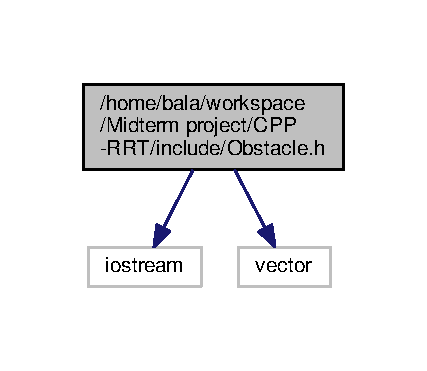
\includegraphics[width=205pt]{Obstacle_8h__incl}
\end{center}
\end{figure}
This graph shows which files directly or indirectly include this file\+:
\nopagebreak
\begin{figure}[H]
\begin{center}
\leavevmode
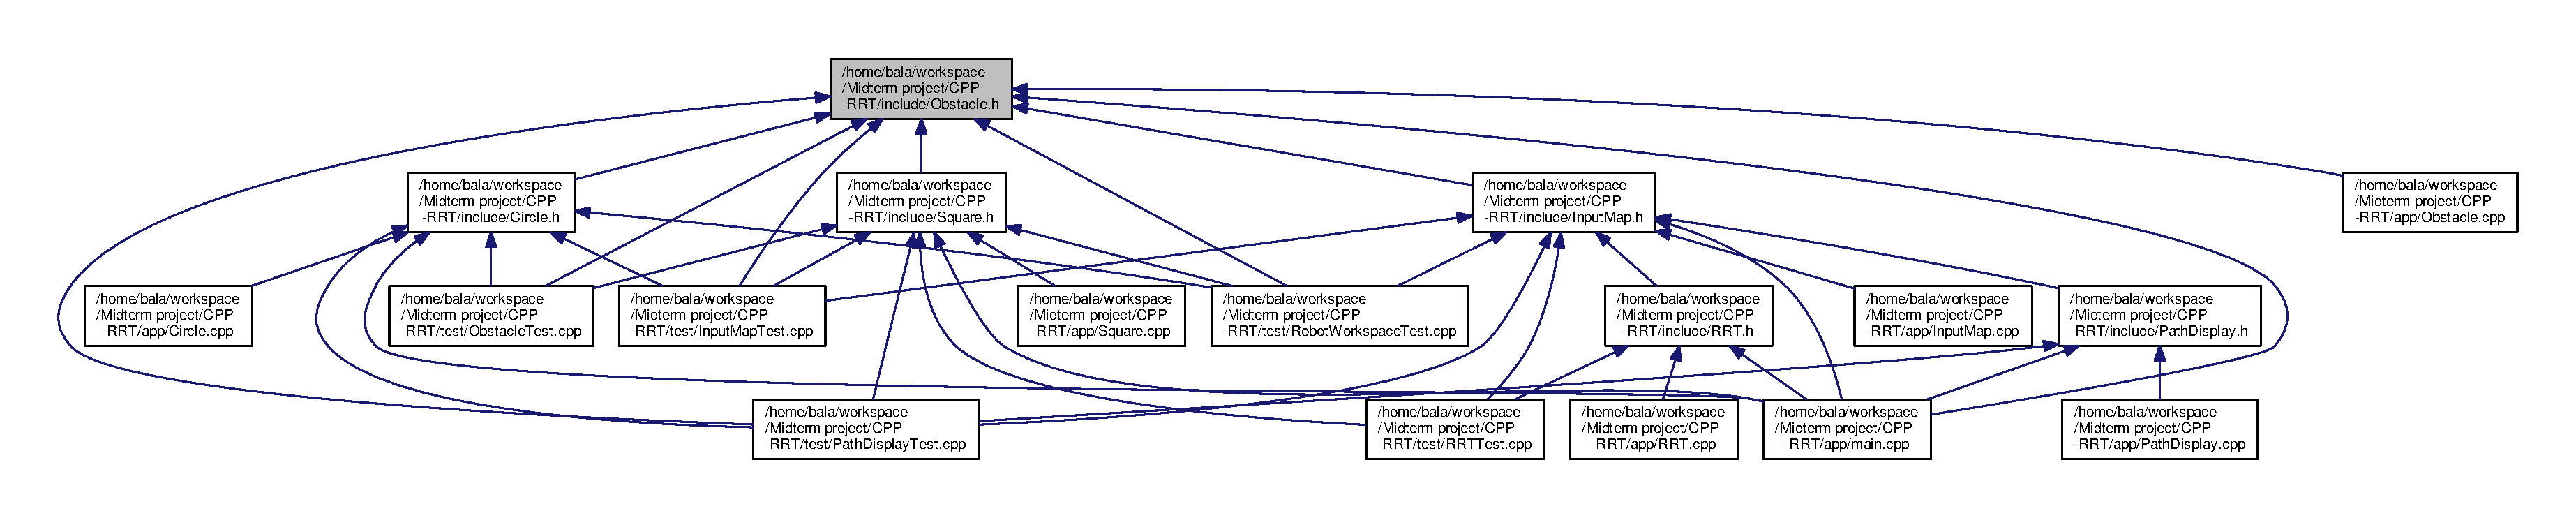
\includegraphics[width=350pt]{Obstacle_8h__dep__incl}
\end{center}
\end{figure}
\subsection*{Classes}
\begin{DoxyCompactItemize}
\item 
struct \hyperlink{structpoint}{point}
\item 
class \hyperlink{classObstacle}{Obstacle}
\begin{DoxyCompactList}\small\item\em \hyperlink{classObstacle}{Obstacle} obstacle class that serves as parent for all types of obstacles. \end{DoxyCompactList}\end{DoxyCompactItemize}

\hypertarget{PathDisplay_8h}{}\section{/home/bala/workspace/\+Midterm project/\+C\+P\+P-\/\+R\+R\+T/include/\+Path\+Display.h File Reference}
\label{PathDisplay_8h}\index{/home/bala/workspace/\+Midterm project/\+C\+P\+P-\/\+R\+R\+T/include/\+Path\+Display.\+h@{/home/bala/workspace/\+Midterm project/\+C\+P\+P-\/\+R\+R\+T/include/\+Path\+Display.\+h}}
{\ttfamily \#include $<$vector$>$}\\*
{\ttfamily \#include $<$memory$>$}\\*
{\ttfamily \#include \char`\"{}../include/\+Input\+Map.\+h\char`\"{}}\\*
Include dependency graph for Path\+Display.\+h\+:
\nopagebreak
\begin{figure}[H]
\begin{center}
\leavevmode
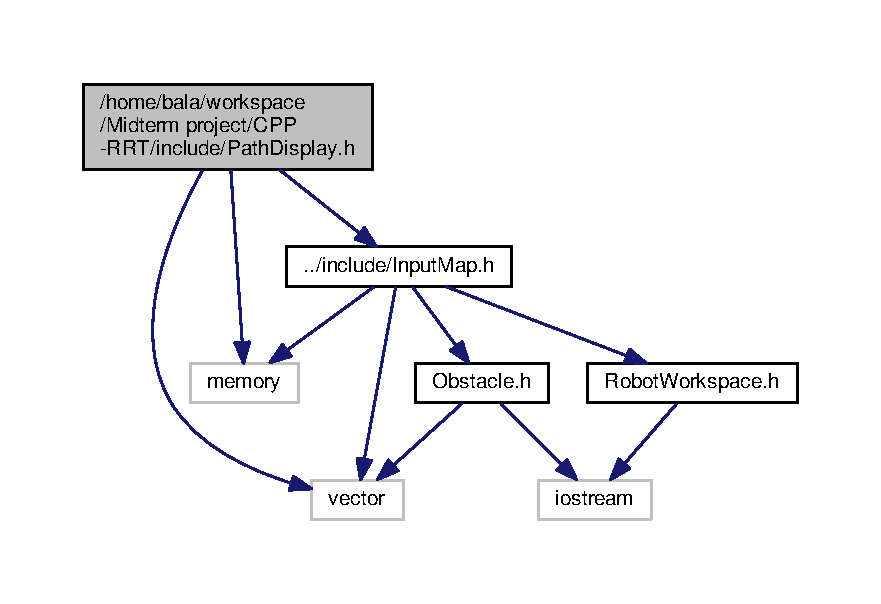
\includegraphics[width=350pt]{PathDisplay_8h__incl}
\end{center}
\end{figure}
This graph shows which files directly or indirectly include this file\+:
\nopagebreak
\begin{figure}[H]
\begin{center}
\leavevmode
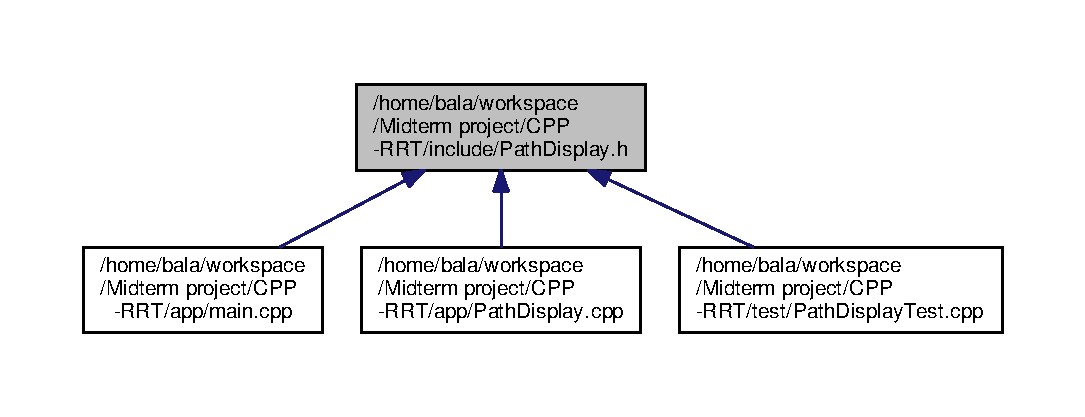
\includegraphics[width=350pt]{PathDisplay_8h__dep__incl}
\end{center}
\end{figure}
\subsection*{Classes}
\begin{DoxyCompactItemize}
\item 
class \hyperlink{classPathDisplay}{Path\+Display}
\begin{DoxyCompactList}\small\item\em Class to display path along with arena to user. \end{DoxyCompactList}\end{DoxyCompactItemize}

\hypertarget{RobotWorkspace_8h}{}\section{/home/bala/workspace/\+Midterm project/\+C\+P\+P-\/\+R\+R\+T/include/\+Robot\+Workspace.h File Reference}
\label{RobotWorkspace_8h}\index{/home/bala/workspace/\+Midterm project/\+C\+P\+P-\/\+R\+R\+T/include/\+Robot\+Workspace.\+h@{/home/bala/workspace/\+Midterm project/\+C\+P\+P-\/\+R\+R\+T/include/\+Robot\+Workspace.\+h}}
{\ttfamily \#include $<$iostream$>$}\\*
Include dependency graph for Robot\+Workspace.\+h\+:
\nopagebreak
\begin{figure}[H]
\begin{center}
\leavevmode
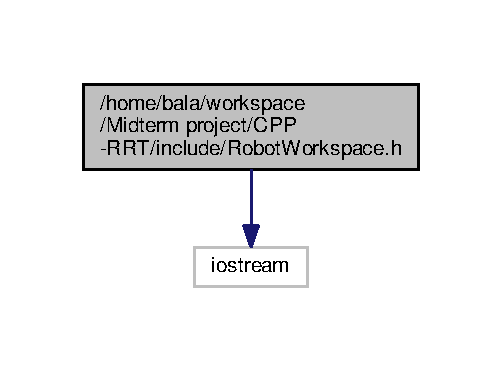
\includegraphics[width=241pt]{RobotWorkspace_8h__incl}
\end{center}
\end{figure}
This graph shows which files directly or indirectly include this file\+:
\nopagebreak
\begin{figure}[H]
\begin{center}
\leavevmode
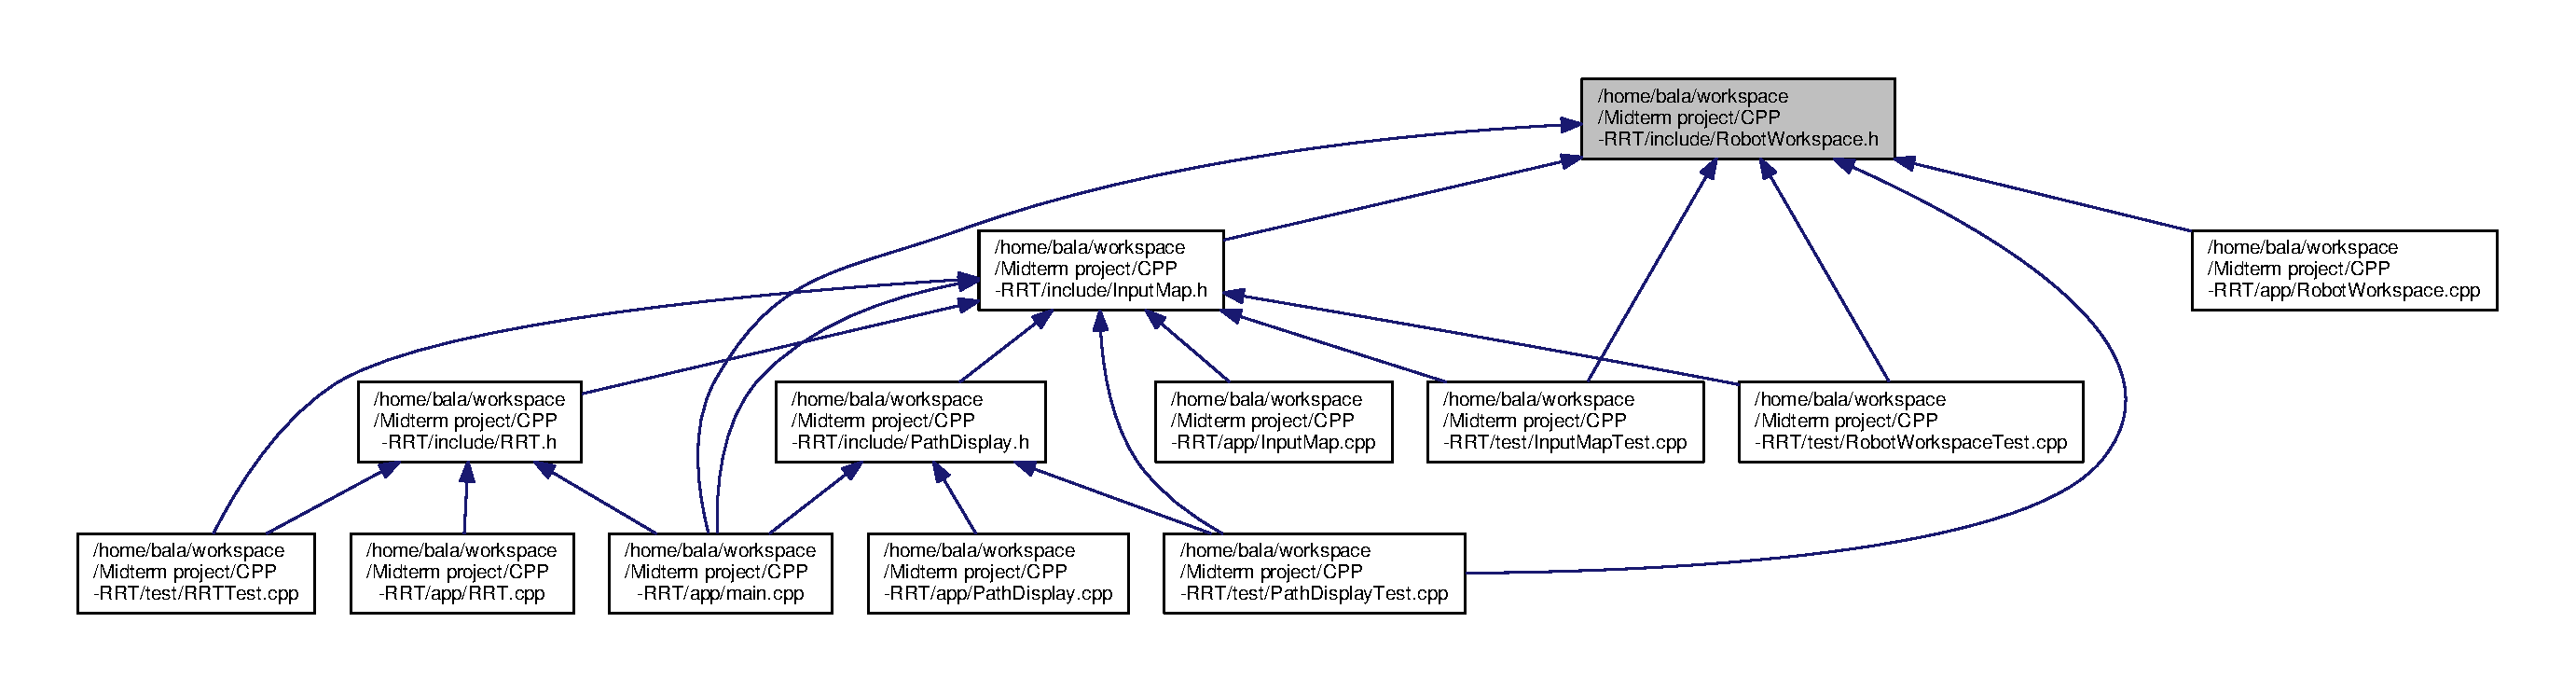
\includegraphics[width=350pt]{RobotWorkspace_8h__dep__incl}
\end{center}
\end{figure}
\subsection*{Classes}
\begin{DoxyCompactItemize}
\item 
class \hyperlink{classRobotWorkspace}{Robot\+Workspace}
\begin{DoxyCompactList}\small\item\em Class holds arena properties. \end{DoxyCompactList}\end{DoxyCompactItemize}

\hypertarget{RRT_8h}{}\section{/home/bala/workspace/\+Midterm project/\+C\+P\+P-\/\+R\+R\+T/include/\+R\+RT.h File Reference}
\label{RRT_8h}\index{/home/bala/workspace/\+Midterm project/\+C\+P\+P-\/\+R\+R\+T/include/\+R\+R\+T.\+h@{/home/bala/workspace/\+Midterm project/\+C\+P\+P-\/\+R\+R\+T/include/\+R\+R\+T.\+h}}
{\ttfamily \#include $<$vector$>$}\\*
{\ttfamily \#include $<$cstdlib$>$}\\*
{\ttfamily \#include $<$ctime$>$}\\*
{\ttfamily \#include $<$algorithm$>$}\\*
{\ttfamily \#include $<$memory$>$}\\*
{\ttfamily \#include \char`\"{}Input\+Map.\+h\char`\"{}}\\*
Include dependency graph for R\+R\+T.\+h\+:\nopagebreak
\begin{figure}[H]
\begin{center}
\leavevmode
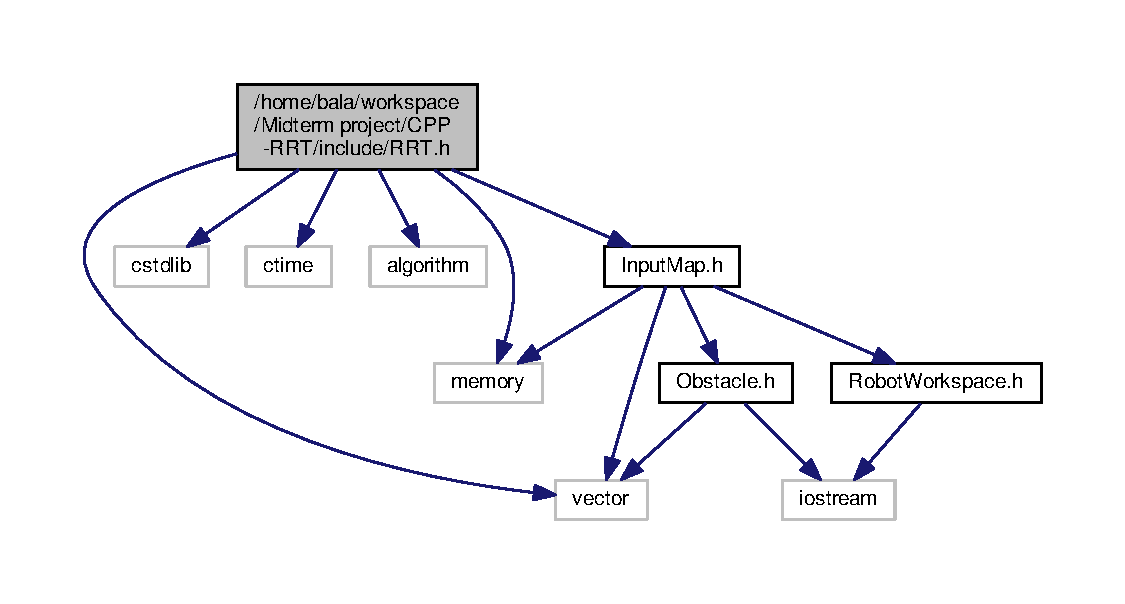
\includegraphics[width=350pt]{RRT_8h__incl}
\end{center}
\end{figure}
This graph shows which files directly or indirectly include this file\+:\nopagebreak
\begin{figure}[H]
\begin{center}
\leavevmode
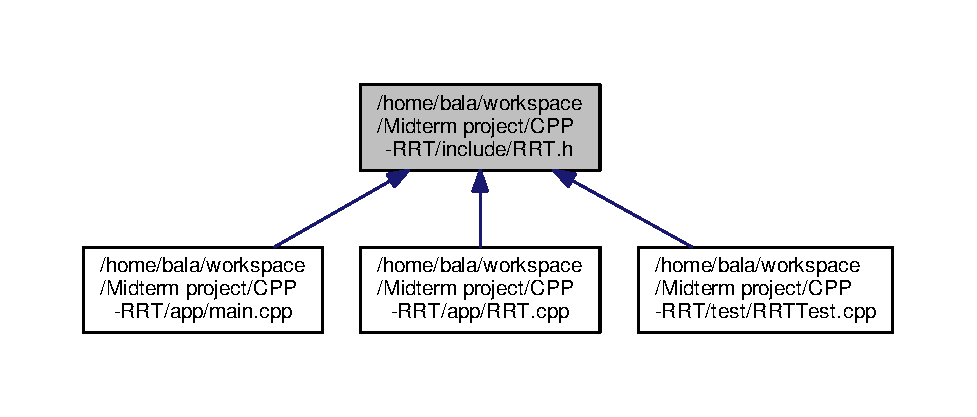
\includegraphics[width=350pt]{RRT_8h__dep__incl}
\end{center}
\end{figure}
\subsection*{Classes}
\begin{DoxyCompactItemize}
\item 
class \hyperlink{classRRT}{R\+RT}
\begin{DoxyCompactList}\small\item\em Class finds path. \end{DoxyCompactList}\end{DoxyCompactItemize}

\hypertarget{Square_8h}{}\section{/home/bala/workspace/\+Midterm project/\+C\+P\+P-\/\+R\+R\+T/include/\+Square.h File Reference}
\label{Square_8h}\index{/home/bala/workspace/\+Midterm project/\+C\+P\+P-\/\+R\+R\+T/include/\+Square.\+h@{/home/bala/workspace/\+Midterm project/\+C\+P\+P-\/\+R\+R\+T/include/\+Square.\+h}}
{\ttfamily \#include $<$iostream$>$}\\*
{\ttfamily \#include $<$vector$>$}\\*
{\ttfamily \#include \char`\"{}Obstacle.\+h\char`\"{}}\\*
Include dependency graph for Square.\+h\+:\nopagebreak
\begin{figure}[H]
\begin{center}
\leavevmode
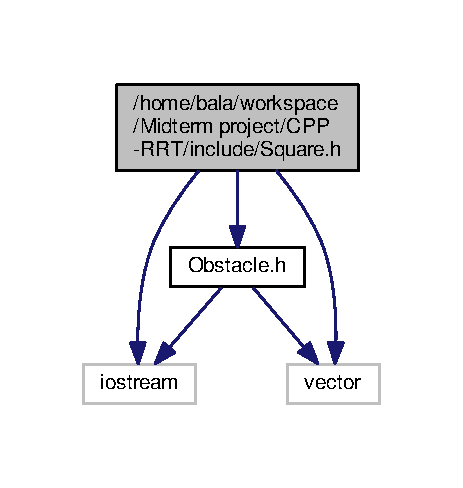
\includegraphics[width=222pt]{Square_8h__incl}
\end{center}
\end{figure}
This graph shows which files directly or indirectly include this file\+:\nopagebreak
\begin{figure}[H]
\begin{center}
\leavevmode
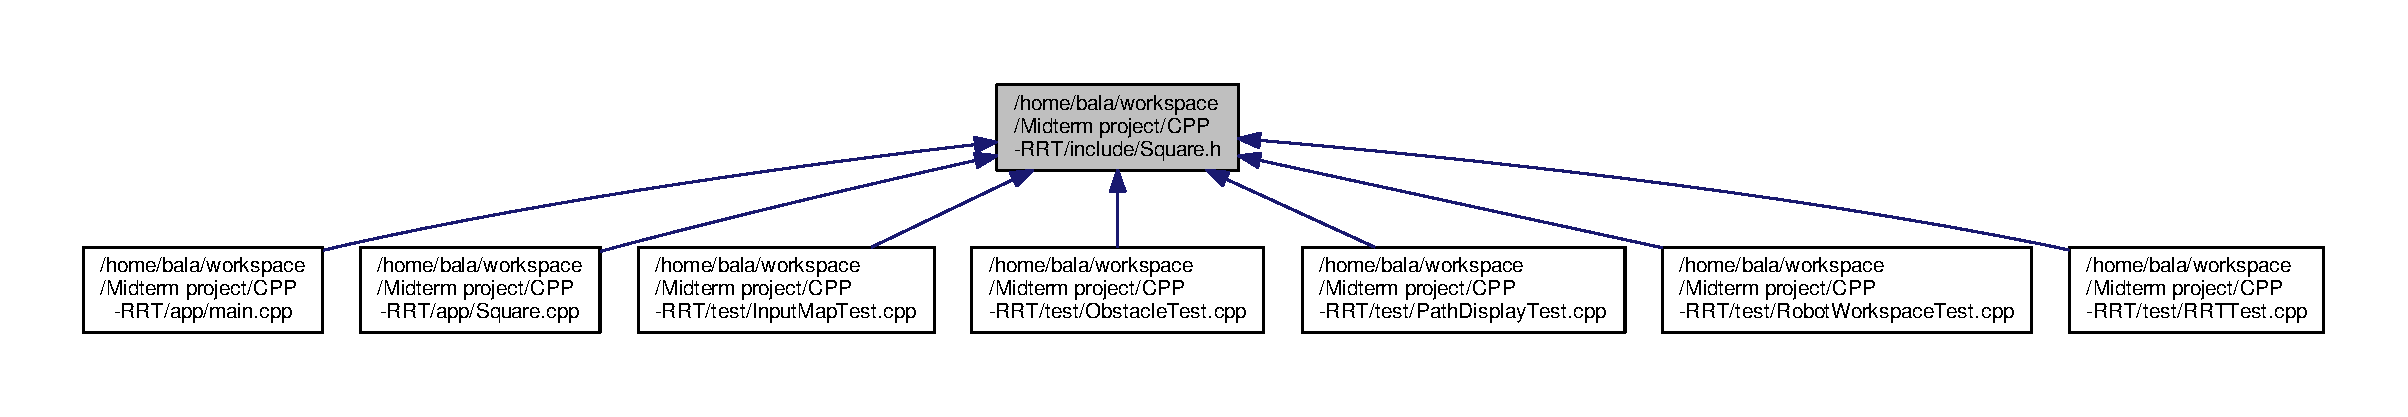
\includegraphics[width=350pt]{Square_8h__dep__incl}
\end{center}
\end{figure}
\subsection*{Classes}
\begin{DoxyCompactItemize}
\item 
class \hyperlink{classSquare}{Square}
\begin{DoxyCompactList}\small\item\em \hyperlink{classSquare}{Square} class that holds functions of \hyperlink{classSquare}{Square} obstacle. \end{DoxyCompactList}\end{DoxyCompactItemize}

\hypertarget{InputMapTest_8cpp}{}\section{/home/bala/workspace/\+Midterm project/\+C\+P\+P-\/\+R\+R\+T/test/\+Input\+Map\+Test.cpp File Reference}
\label{InputMapTest_8cpp}\index{/home/bala/workspace/\+Midterm project/\+C\+P\+P-\/\+R\+R\+T/test/\+Input\+Map\+Test.\+cpp@{/home/bala/workspace/\+Midterm project/\+C\+P\+P-\/\+R\+R\+T/test/\+Input\+Map\+Test.\+cpp}}
{\ttfamily \#include $<$gtest/gtest.\+h$>$}\\*
{\ttfamily \#include $<$sstream$>$}\\*
{\ttfamily \#include $<$iostream$>$}\\*
{\ttfamily \#include $<$string$>$}\\*
{\ttfamily \#include $<$vector$>$}\\*
{\ttfamily \#include \char`\"{}../include/\+Input\+Map.\+h\char`\"{}}\\*
{\ttfamily \#include \char`\"{}../include/\+Robot\+Workspace.\+h\char`\"{}}\\*
{\ttfamily \#include \char`\"{}../include/\+Obstacle.\+h\char`\"{}}\\*
{\ttfamily \#include \char`\"{}../include/\+Square.\+h\char`\"{}}\\*
{\ttfamily \#include \char`\"{}../include/\+Circle.\+h\char`\"{}}\\*
Include dependency graph for Input\+Map\+Test.\+cpp\+:\nopagebreak
\begin{figure}[H]
\begin{center}
\leavevmode
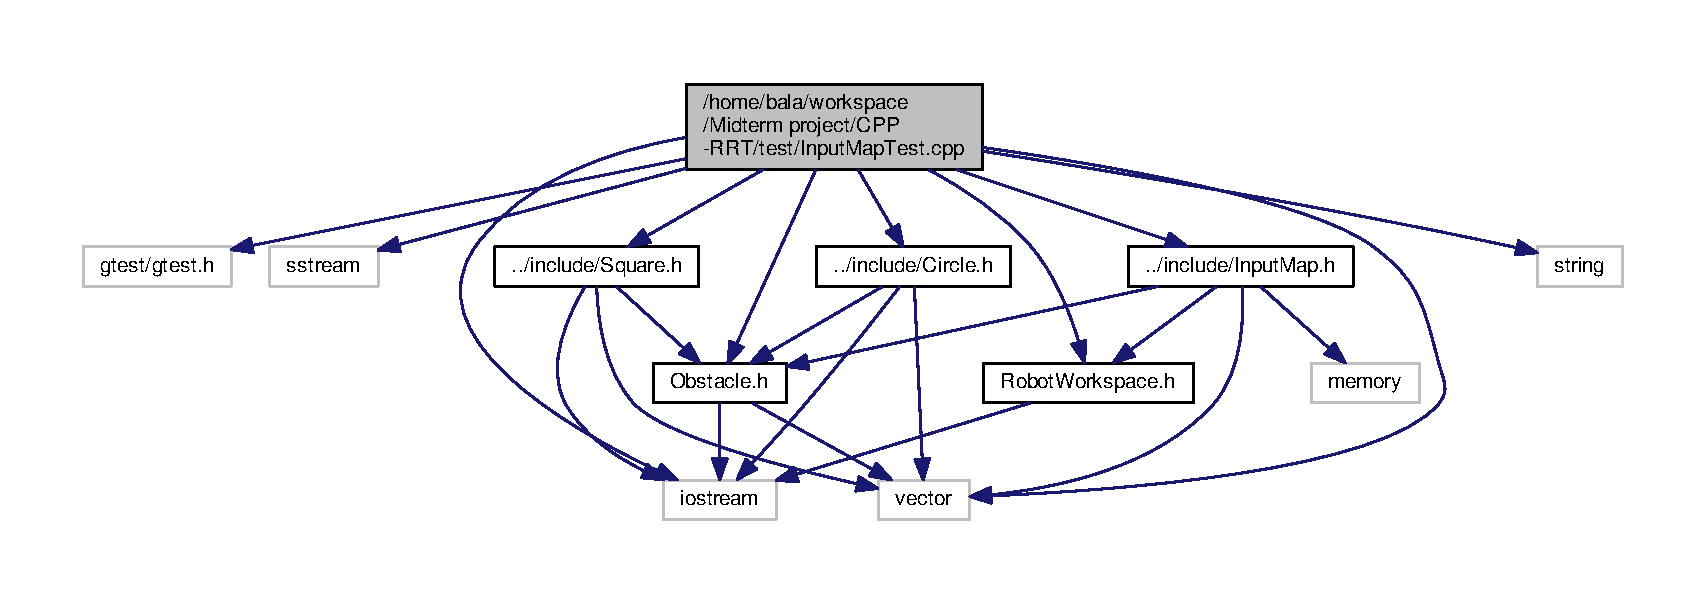
\includegraphics[width=350pt]{InputMapTest_8cpp__incl}
\end{center}
\end{figure}
\subsection*{Functions}
\begin{DoxyCompactItemize}
\item 
\hyperlink{InputMapTest_8cpp_aa50172b2654d99240e8866b21243d337}{T\+E\+ST} (Input\+Mapclass, Config\+Space\+Creation)
\begin{DoxyCompactList}\small\item\em Testing input map computation. \end{DoxyCompactList}\item 
\hyperlink{InputMapTest_8cpp_a0848952f1fa141017f2704ea3f72eb98}{T\+E\+ST} (Input\+Mapclass, Set\+Workspace\+Test)
\begin{DoxyCompactList}\small\item\em Testing input map Set Workspace. \end{DoxyCompactList}\item 
\hyperlink{InputMapTest_8cpp_a7c2552a954c885b7ac07f6f97e339844}{T\+E\+ST} (Input\+Mapclass, Add\+Obstacle\+Test)
\begin{DoxyCompactList}\small\item\em Testing obstacle. \end{DoxyCompactList}\end{DoxyCompactItemize}


\subsection{Function Documentation}
\index{Input\+Map\+Test.\+cpp@{Input\+Map\+Test.\+cpp}!T\+E\+ST@{T\+E\+ST}}
\index{T\+E\+ST@{T\+E\+ST}!Input\+Map\+Test.\+cpp@{Input\+Map\+Test.\+cpp}}
\subsubsection[{\texorpdfstring{T\+E\+S\+T(\+Input\+Mapclass, Config\+Space\+Creation)}{TEST(InputMapclass, ConfigSpaceCreation)}}]{\setlength{\rightskip}{0pt plus 5cm}T\+E\+ST (
\begin{DoxyParamCaption}
\item[{Input\+Mapclass}]{, }
\item[{Config\+Space\+Creation}]{}
\end{DoxyParamCaption}
)}\hypertarget{InputMapTest_8cpp_aa50172b2654d99240e8866b21243d337}{}\label{InputMapTest_8cpp_aa50172b2654d99240e8866b21243d337}


Testing input map computation. 

\index{Input\+Map\+Test.\+cpp@{Input\+Map\+Test.\+cpp}!T\+E\+ST@{T\+E\+ST}}
\index{T\+E\+ST@{T\+E\+ST}!Input\+Map\+Test.\+cpp@{Input\+Map\+Test.\+cpp}}
\subsubsection[{\texorpdfstring{T\+E\+S\+T(\+Input\+Mapclass, Set\+Workspace\+Test)}{TEST(InputMapclass, SetWorkspaceTest)}}]{\setlength{\rightskip}{0pt plus 5cm}T\+E\+ST (
\begin{DoxyParamCaption}
\item[{Input\+Mapclass}]{, }
\item[{Set\+Workspace\+Test}]{}
\end{DoxyParamCaption}
)}\hypertarget{InputMapTest_8cpp_a0848952f1fa141017f2704ea3f72eb98}{}\label{InputMapTest_8cpp_a0848952f1fa141017f2704ea3f72eb98}


Testing input map Set Workspace. 

\index{Input\+Map\+Test.\+cpp@{Input\+Map\+Test.\+cpp}!T\+E\+ST@{T\+E\+ST}}
\index{T\+E\+ST@{T\+E\+ST}!Input\+Map\+Test.\+cpp@{Input\+Map\+Test.\+cpp}}
\subsubsection[{\texorpdfstring{T\+E\+S\+T(\+Input\+Mapclass, Add\+Obstacle\+Test)}{TEST(InputMapclass, AddObstacleTest)}}]{\setlength{\rightskip}{0pt plus 5cm}T\+E\+ST (
\begin{DoxyParamCaption}
\item[{Input\+Mapclass}]{, }
\item[{Add\+Obstacle\+Test}]{}
\end{DoxyParamCaption}
)}\hypertarget{InputMapTest_8cpp_a7c2552a954c885b7ac07f6f97e339844}{}\label{InputMapTest_8cpp_a7c2552a954c885b7ac07f6f97e339844}


Testing obstacle. 


\hypertarget{ObstacleTest_8cpp}{}\section{/home/bala/workspace/\+Midterm project/\+C\+P\+P-\/\+R\+R\+T/test/\+Obstacle\+Test.cpp File Reference}
\label{ObstacleTest_8cpp}\index{/home/bala/workspace/\+Midterm project/\+C\+P\+P-\/\+R\+R\+T/test/\+Obstacle\+Test.\+cpp@{/home/bala/workspace/\+Midterm project/\+C\+P\+P-\/\+R\+R\+T/test/\+Obstacle\+Test.\+cpp}}
{\ttfamily \#include $<$gtest/gtest.\+h$>$}\\*
{\ttfamily \#include $<$sstream$>$}\\*
{\ttfamily \#include $<$iostream$>$}\\*
{\ttfamily \#include $<$string$>$}\\*
{\ttfamily \#include \char`\"{}../include/\+Obstacle.\+h\char`\"{}}\\*
{\ttfamily \#include \char`\"{}../include/\+Square.\+h\char`\"{}}\\*
{\ttfamily \#include \char`\"{}../include/\+Circle.\+h\char`\"{}}\\*
Include dependency graph for Obstacle\+Test.\+cpp\+:\nopagebreak
\begin{figure}[H]
\begin{center}
\leavevmode
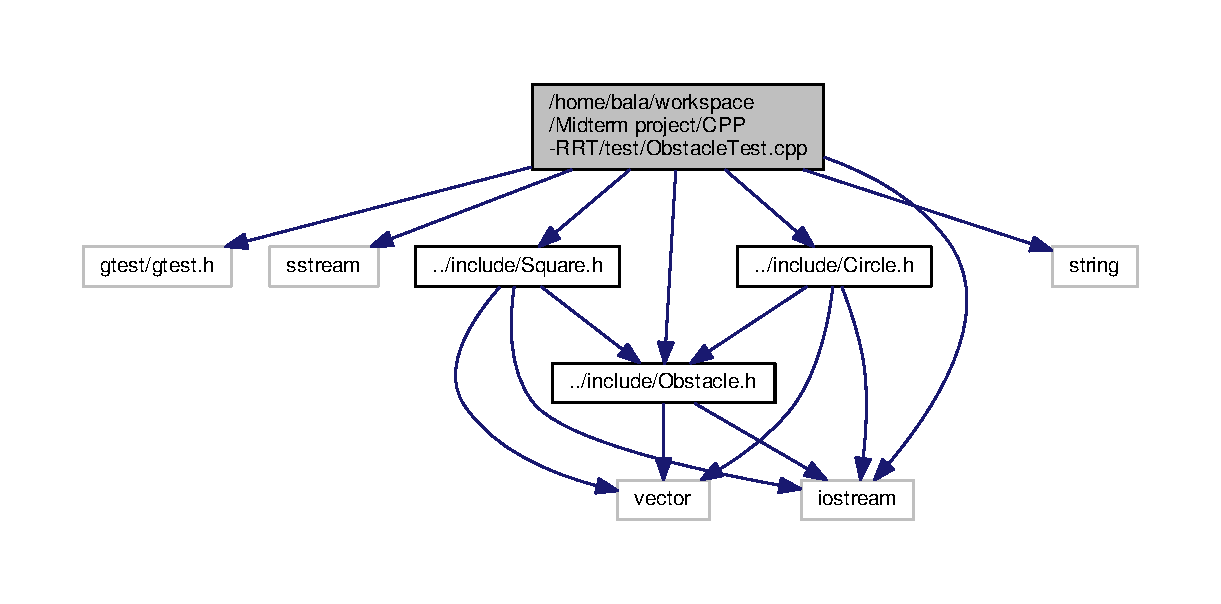
\includegraphics[width=350pt]{ObstacleTest_8cpp__incl}
\end{center}
\end{figure}
\subsection*{Classes}
\begin{DoxyCompactItemize}
\item 
struct \hyperlink{structSquareTest}{Square\+Test}
\begin{DoxyCompactList}\small\item\em \hyperlink{classSquare}{Square} class test fixture. \end{DoxyCompactList}\item 
struct \hyperlink{structCircleTest}{Circle\+Test}
\begin{DoxyCompactList}\small\item\em \hyperlink{classCircle}{Circle} class test fixture. \end{DoxyCompactList}\item 
struct \hyperlink{structObstacleCircleTest}{Obstacle\+Circle\+Test}
\begin{DoxyCompactList}\small\item\em \hyperlink{classObstacle}{Obstacle} \hyperlink{classCircle}{Circle} class test fixture for overriding. \end{DoxyCompactList}\item 
struct \hyperlink{structObstacleSquareTest}{Obstacle\+Square\+Test}
\begin{DoxyCompactList}\small\item\em \hyperlink{classObstacle}{Obstacle} square class test fixture for overriding. \end{DoxyCompactList}\end{DoxyCompactItemize}
\subsection*{Functions}
\begin{DoxyCompactItemize}
\item 
\hyperlink{ObstacleTest_8cpp_afc7bab07ae078a30433e3495d400ac78}{T\+E\+ST} (Square\+Class, Initialization)
\begin{DoxyCompactList}\small\item\em Testing square initialization. \end{DoxyCompactList}\item 
\hyperlink{ObstacleTest_8cpp_a3799eaeeb026b9cae5cad17d3653f4fe}{T\+E\+S\+T\+\_\+F} (\hyperlink{structSquareTest}{Square\+Test}, Inside\+Outside\+Obstacle)
\begin{DoxyCompactList}\small\item\em Testing if point is inside square obstacle or not. \end{DoxyCompactList}\item 
\hyperlink{ObstacleTest_8cpp_a9dd02dfb89d63f1bc692e5743e557224}{T\+E\+S\+T\+\_\+F} (\hyperlink{structSquareTest}{Square\+Test}, Fill\+Square\+Obstacle)
\begin{DoxyCompactList}\small\item\em Testing filling the square obstacle. \end{DoxyCompactList}\item 
\hyperlink{ObstacleTest_8cpp_ab57fedd08ee12ade1a212745f3fa7e25}{T\+E\+ST} (Circle\+Class, Initialization)
\begin{DoxyCompactList}\small\item\em Testing circle initialization. \end{DoxyCompactList}\item 
\hyperlink{ObstacleTest_8cpp_a634e1a3cd0ffa153a42d43ebaabd20fc}{T\+E\+S\+T\+\_\+F} (\hyperlink{structCircleTest}{Circle\+Test}, inside\+Outside\+Obstacle)
\begin{DoxyCompactList}\small\item\em Testing if point is inside circle obstacle or not. \end{DoxyCompactList}\item 
\hyperlink{ObstacleTest_8cpp_aef3eb79545f80091239742ee1a4d4596}{T\+E\+S\+T\+\_\+F} (\hyperlink{structCircleTest}{Circle\+Test}, Fill\+Circle\+Obstacle)
\begin{DoxyCompactList}\small\item\em Testing filling the circle obstacle. \end{DoxyCompactList}\item 
\hyperlink{ObstacleTest_8cpp_a9fd0db3707fb6cfb7fd6bc354b1344d7}{T\+E\+ST} (Obstacle\+Circle\+Class, Initialization)
\begin{DoxyCompactList}\small\item\em Testing circle initialization fir overriding. \end{DoxyCompactList}\item 
\hyperlink{ObstacleTest_8cpp_ac0ab87a7e42b6abd39ba103ec99b4b02}{T\+E\+S\+T\+\_\+F} (\hyperlink{structObstacleCircleTest}{Obstacle\+Circle\+Test}, inside\+Outside\+Obstacle)
\begin{DoxyCompactList}\small\item\em Testing if point is inside circle obstacle or not through overriding. \end{DoxyCompactList}\item 
\hyperlink{ObstacleTest_8cpp_a87923ae54a36a2de1c8a494bce6b3901}{T\+E\+ST} (Obstaclesquare\+Class, Initialization)
\begin{DoxyCompactList}\small\item\em Testing square class initialization for overriding. \end{DoxyCompactList}\item 
\hyperlink{ObstacleTest_8cpp_a185c90335f2880930140c19868132b7e}{T\+E\+S\+T\+\_\+F} (\hyperlink{structObstacleSquareTest}{Obstacle\+Square\+Test}, inside\+Outside\+Obstacle)
\begin{DoxyCompactList}\small\item\em Testing if point is inside circle obstacle or not through overriding. \end{DoxyCompactList}\end{DoxyCompactItemize}


\subsection{Function Documentation}
\index{Obstacle\+Test.\+cpp@{Obstacle\+Test.\+cpp}!T\+E\+ST@{T\+E\+ST}}
\index{T\+E\+ST@{T\+E\+ST}!Obstacle\+Test.\+cpp@{Obstacle\+Test.\+cpp}}
\subsubsection[{\texorpdfstring{T\+E\+S\+T(\+Square\+Class, Initialization)}{TEST(SquareClass, Initialization)}}]{\setlength{\rightskip}{0pt plus 5cm}T\+E\+ST (
\begin{DoxyParamCaption}
\item[{Square\+Class}]{, }
\item[{Initialization}]{}
\end{DoxyParamCaption}
)}\hypertarget{ObstacleTest_8cpp_afc7bab07ae078a30433e3495d400ac78}{}\label{ObstacleTest_8cpp_afc7bab07ae078a30433e3495d400ac78}


Testing square initialization. 

\index{Obstacle\+Test.\+cpp@{Obstacle\+Test.\+cpp}!T\+E\+ST@{T\+E\+ST}}
\index{T\+E\+ST@{T\+E\+ST}!Obstacle\+Test.\+cpp@{Obstacle\+Test.\+cpp}}
\subsubsection[{\texorpdfstring{T\+E\+S\+T(\+Circle\+Class, Initialization)}{TEST(CircleClass, Initialization)}}]{\setlength{\rightskip}{0pt plus 5cm}T\+E\+ST (
\begin{DoxyParamCaption}
\item[{Circle\+Class}]{, }
\item[{Initialization}]{}
\end{DoxyParamCaption}
)}\hypertarget{ObstacleTest_8cpp_ab57fedd08ee12ade1a212745f3fa7e25}{}\label{ObstacleTest_8cpp_ab57fedd08ee12ade1a212745f3fa7e25}


Testing circle initialization. 

\index{Obstacle\+Test.\+cpp@{Obstacle\+Test.\+cpp}!T\+E\+ST@{T\+E\+ST}}
\index{T\+E\+ST@{T\+E\+ST}!Obstacle\+Test.\+cpp@{Obstacle\+Test.\+cpp}}
\subsubsection[{\texorpdfstring{T\+E\+S\+T(\+Obstacle\+Circle\+Class, Initialization)}{TEST(ObstacleCircleClass, Initialization)}}]{\setlength{\rightskip}{0pt plus 5cm}T\+E\+ST (
\begin{DoxyParamCaption}
\item[{Obstacle\+Circle\+Class}]{, }
\item[{Initialization}]{}
\end{DoxyParamCaption}
)}\hypertarget{ObstacleTest_8cpp_a9fd0db3707fb6cfb7fd6bc354b1344d7}{}\label{ObstacleTest_8cpp_a9fd0db3707fb6cfb7fd6bc354b1344d7}


Testing circle initialization fir overriding. 

\index{Obstacle\+Test.\+cpp@{Obstacle\+Test.\+cpp}!T\+E\+ST@{T\+E\+ST}}
\index{T\+E\+ST@{T\+E\+ST}!Obstacle\+Test.\+cpp@{Obstacle\+Test.\+cpp}}
\subsubsection[{\texorpdfstring{T\+E\+S\+T(\+Obstaclesquare\+Class, Initialization)}{TEST(ObstaclesquareClass, Initialization)}}]{\setlength{\rightskip}{0pt plus 5cm}T\+E\+ST (
\begin{DoxyParamCaption}
\item[{Obstaclesquare\+Class}]{, }
\item[{Initialization}]{}
\end{DoxyParamCaption}
)}\hypertarget{ObstacleTest_8cpp_a87923ae54a36a2de1c8a494bce6b3901}{}\label{ObstacleTest_8cpp_a87923ae54a36a2de1c8a494bce6b3901}


Testing square class initialization for overriding. 

\index{Obstacle\+Test.\+cpp@{Obstacle\+Test.\+cpp}!T\+E\+S\+T\+\_\+F@{T\+E\+S\+T\+\_\+F}}
\index{T\+E\+S\+T\+\_\+F@{T\+E\+S\+T\+\_\+F}!Obstacle\+Test.\+cpp@{Obstacle\+Test.\+cpp}}
\subsubsection[{\texorpdfstring{T\+E\+S\+T\+\_\+\+F(\+Square\+Test, Inside\+Outside\+Obstacle)}{TEST_F(SquareTest, InsideOutsideObstacle)}}]{\setlength{\rightskip}{0pt plus 5cm}T\+E\+S\+T\+\_\+F (
\begin{DoxyParamCaption}
\item[{{\bf Square\+Test}}]{, }
\item[{Inside\+Outside\+Obstacle}]{}
\end{DoxyParamCaption}
)}\hypertarget{ObstacleTest_8cpp_a3799eaeeb026b9cae5cad17d3653f4fe}{}\label{ObstacleTest_8cpp_a3799eaeeb026b9cae5cad17d3653f4fe}


Testing if point is inside square obstacle or not. 

\index{Obstacle\+Test.\+cpp@{Obstacle\+Test.\+cpp}!T\+E\+S\+T\+\_\+F@{T\+E\+S\+T\+\_\+F}}
\index{T\+E\+S\+T\+\_\+F@{T\+E\+S\+T\+\_\+F}!Obstacle\+Test.\+cpp@{Obstacle\+Test.\+cpp}}
\subsubsection[{\texorpdfstring{T\+E\+S\+T\+\_\+\+F(\+Square\+Test, Fill\+Square\+Obstacle)}{TEST_F(SquareTest, FillSquareObstacle)}}]{\setlength{\rightskip}{0pt plus 5cm}T\+E\+S\+T\+\_\+F (
\begin{DoxyParamCaption}
\item[{{\bf Square\+Test}}]{, }
\item[{Fill\+Square\+Obstacle}]{}
\end{DoxyParamCaption}
)}\hypertarget{ObstacleTest_8cpp_a9dd02dfb89d63f1bc692e5743e557224}{}\label{ObstacleTest_8cpp_a9dd02dfb89d63f1bc692e5743e557224}


Testing filling the square obstacle. 

\index{Obstacle\+Test.\+cpp@{Obstacle\+Test.\+cpp}!T\+E\+S\+T\+\_\+F@{T\+E\+S\+T\+\_\+F}}
\index{T\+E\+S\+T\+\_\+F@{T\+E\+S\+T\+\_\+F}!Obstacle\+Test.\+cpp@{Obstacle\+Test.\+cpp}}
\subsubsection[{\texorpdfstring{T\+E\+S\+T\+\_\+\+F(\+Circle\+Test, inside\+Outside\+Obstacle)}{TEST_F(CircleTest, insideOutsideObstacle)}}]{\setlength{\rightskip}{0pt plus 5cm}T\+E\+S\+T\+\_\+F (
\begin{DoxyParamCaption}
\item[{{\bf Circle\+Test}}]{, }
\item[{inside\+Outside\+Obstacle}]{}
\end{DoxyParamCaption}
)}\hypertarget{ObstacleTest_8cpp_a634e1a3cd0ffa153a42d43ebaabd20fc}{}\label{ObstacleTest_8cpp_a634e1a3cd0ffa153a42d43ebaabd20fc}


Testing if point is inside circle obstacle or not. 

\index{Obstacle\+Test.\+cpp@{Obstacle\+Test.\+cpp}!T\+E\+S\+T\+\_\+F@{T\+E\+S\+T\+\_\+F}}
\index{T\+E\+S\+T\+\_\+F@{T\+E\+S\+T\+\_\+F}!Obstacle\+Test.\+cpp@{Obstacle\+Test.\+cpp}}
\subsubsection[{\texorpdfstring{T\+E\+S\+T\+\_\+\+F(\+Circle\+Test, Fill\+Circle\+Obstacle)}{TEST_F(CircleTest, FillCircleObstacle)}}]{\setlength{\rightskip}{0pt plus 5cm}T\+E\+S\+T\+\_\+F (
\begin{DoxyParamCaption}
\item[{{\bf Circle\+Test}}]{, }
\item[{Fill\+Circle\+Obstacle}]{}
\end{DoxyParamCaption}
)}\hypertarget{ObstacleTest_8cpp_aef3eb79545f80091239742ee1a4d4596}{}\label{ObstacleTest_8cpp_aef3eb79545f80091239742ee1a4d4596}


Testing filling the circle obstacle. 

\index{Obstacle\+Test.\+cpp@{Obstacle\+Test.\+cpp}!T\+E\+S\+T\+\_\+F@{T\+E\+S\+T\+\_\+F}}
\index{T\+E\+S\+T\+\_\+F@{T\+E\+S\+T\+\_\+F}!Obstacle\+Test.\+cpp@{Obstacle\+Test.\+cpp}}
\subsubsection[{\texorpdfstring{T\+E\+S\+T\+\_\+\+F(\+Obstacle\+Circle\+Test, inside\+Outside\+Obstacle)}{TEST_F(ObstacleCircleTest, insideOutsideObstacle)}}]{\setlength{\rightskip}{0pt plus 5cm}T\+E\+S\+T\+\_\+F (
\begin{DoxyParamCaption}
\item[{{\bf Obstacle\+Circle\+Test}}]{, }
\item[{inside\+Outside\+Obstacle}]{}
\end{DoxyParamCaption}
)}\hypertarget{ObstacleTest_8cpp_ac0ab87a7e42b6abd39ba103ec99b4b02}{}\label{ObstacleTest_8cpp_ac0ab87a7e42b6abd39ba103ec99b4b02}


Testing if point is inside circle obstacle or not through overriding. 

\index{Obstacle\+Test.\+cpp@{Obstacle\+Test.\+cpp}!T\+E\+S\+T\+\_\+F@{T\+E\+S\+T\+\_\+F}}
\index{T\+E\+S\+T\+\_\+F@{T\+E\+S\+T\+\_\+F}!Obstacle\+Test.\+cpp@{Obstacle\+Test.\+cpp}}
\subsubsection[{\texorpdfstring{T\+E\+S\+T\+\_\+\+F(\+Obstacle\+Square\+Test, inside\+Outside\+Obstacle)}{TEST_F(ObstacleSquareTest, insideOutsideObstacle)}}]{\setlength{\rightskip}{0pt plus 5cm}T\+E\+S\+T\+\_\+F (
\begin{DoxyParamCaption}
\item[{{\bf Obstacle\+Square\+Test}}]{, }
\item[{inside\+Outside\+Obstacle}]{}
\end{DoxyParamCaption}
)}\hypertarget{ObstacleTest_8cpp_a185c90335f2880930140c19868132b7e}{}\label{ObstacleTest_8cpp_a185c90335f2880930140c19868132b7e}


Testing if point is inside circle obstacle or not through overriding. 


\hypertarget{PathDisplayTest_8cpp}{}\section{/home/bala/workspace/\+Midterm project/\+C\+P\+P-\/\+R\+R\+T/test/\+Path\+Display\+Test.cpp File Reference}
\label{PathDisplayTest_8cpp}\index{/home/bala/workspace/\+Midterm project/\+C\+P\+P-\/\+R\+R\+T/test/\+Path\+Display\+Test.\+cpp@{/home/bala/workspace/\+Midterm project/\+C\+P\+P-\/\+R\+R\+T/test/\+Path\+Display\+Test.\+cpp}}
{\ttfamily \#include $<$gtest/gtest.\+h$>$}\\*
{\ttfamily \#include $<$sstream$>$}\\*
{\ttfamily \#include $<$iostream$>$}\\*
{\ttfamily \#include $<$string$>$}\\*
{\ttfamily \#include $<$memory$>$}\\*
{\ttfamily \#include \char`\"{}../include/\+Input\+Map.\+h\char`\"{}}\\*
{\ttfamily \#include \char`\"{}../include/\+Robot\+Workspace.\+h\char`\"{}}\\*
{\ttfamily \#include \char`\"{}../include/\+Obstacle.\+h\char`\"{}}\\*
{\ttfamily \#include \char`\"{}../include/\+Square.\+h\char`\"{}}\\*
{\ttfamily \#include \char`\"{}../include/\+Circle.\+h\char`\"{}}\\*
{\ttfamily \#include \char`\"{}../include/\+Path\+Display.\+h\char`\"{}}\\*
Include dependency graph for Path\+Display\+Test.\+cpp\+:\nopagebreak
\begin{figure}[H]
\begin{center}
\leavevmode
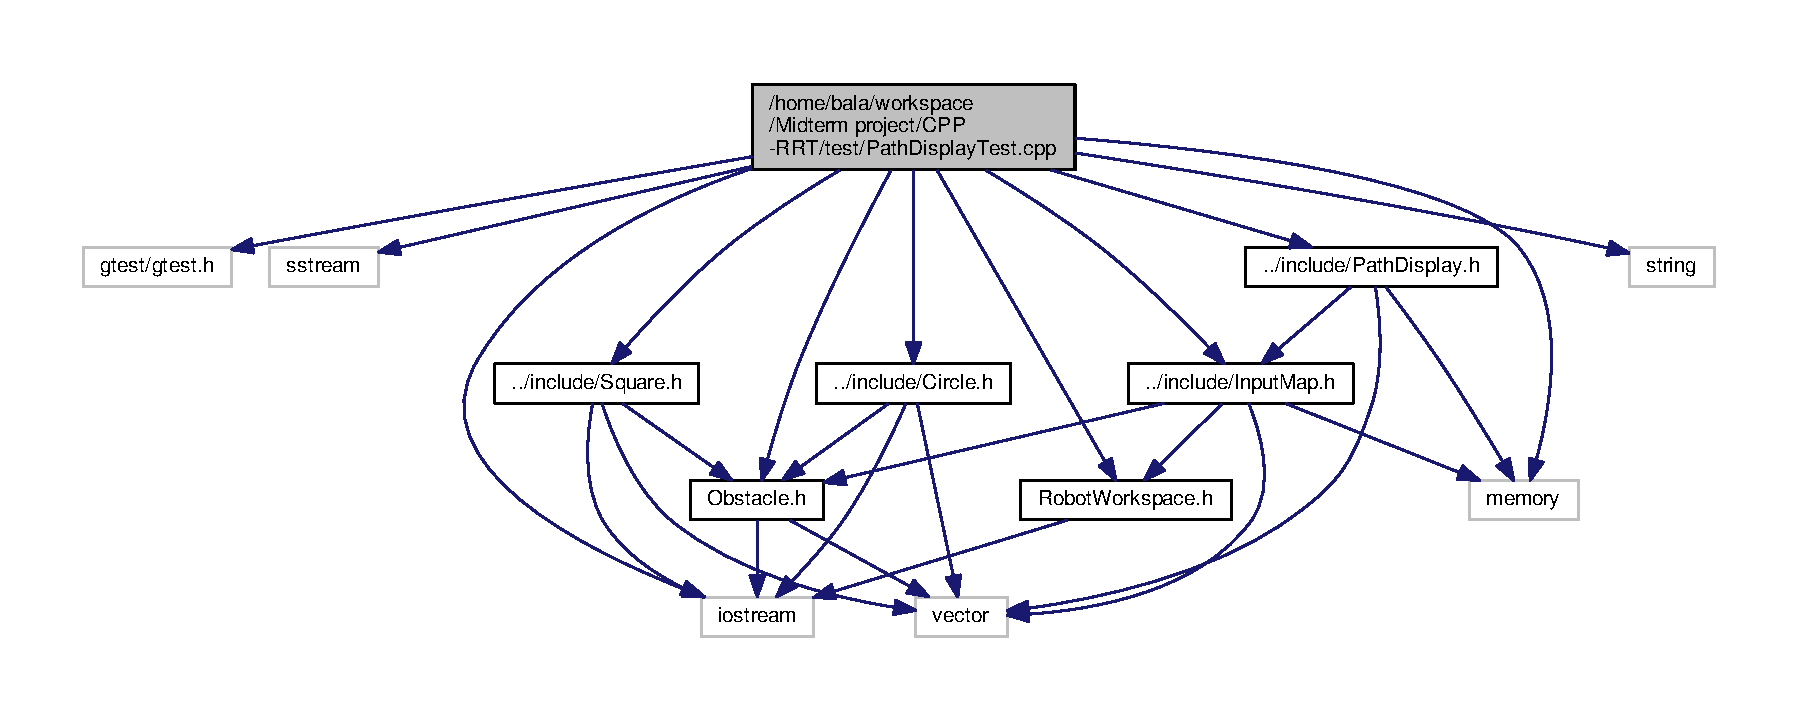
\includegraphics[width=350pt]{PathDisplayTest_8cpp__incl}
\end{center}
\end{figure}
\subsection*{Functions}
\begin{DoxyCompactItemize}
\item 
\hyperlink{PathDisplayTest_8cpp_a0aa954de7be0f393a4aba5ad22b84afd}{T\+E\+ST} (Path\+Display\+Class, Config\+Space\+Creation)
\begin{DoxyCompactList}\small\item\em Path Display. \end{DoxyCompactList}\end{DoxyCompactItemize}


\subsection{Function Documentation}
\index{Path\+Display\+Test.\+cpp@{Path\+Display\+Test.\+cpp}!T\+E\+ST@{T\+E\+ST}}
\index{T\+E\+ST@{T\+E\+ST}!Path\+Display\+Test.\+cpp@{Path\+Display\+Test.\+cpp}}
\subsubsection[{\texorpdfstring{T\+E\+S\+T(\+Path\+Display\+Class, Config\+Space\+Creation)}{TEST(PathDisplayClass, ConfigSpaceCreation)}}]{\setlength{\rightskip}{0pt plus 5cm}T\+E\+ST (
\begin{DoxyParamCaption}
\item[{Path\+Display\+Class}]{, }
\item[{Config\+Space\+Creation}]{}
\end{DoxyParamCaption}
)}\hypertarget{PathDisplayTest_8cpp_a0aa954de7be0f393a4aba5ad22b84afd}{}\label{PathDisplayTest_8cpp_a0aa954de7be0f393a4aba5ad22b84afd}


Path Display. 


\hypertarget{RobotWorkspaceTest_8cpp}{}\section{/home/bala/workspace/\+Midterm project/\+C\+P\+P-\/\+R\+R\+T/test/\+Robot\+Workspace\+Test.cpp File Reference}
\label{RobotWorkspaceTest_8cpp}\index{/home/bala/workspace/\+Midterm project/\+C\+P\+P-\/\+R\+R\+T/test/\+Robot\+Workspace\+Test.\+cpp@{/home/bala/workspace/\+Midterm project/\+C\+P\+P-\/\+R\+R\+T/test/\+Robot\+Workspace\+Test.\+cpp}}
{\ttfamily \#include $<$gtest/gtest.\+h$>$}\\*
{\ttfamily \#include $<$sstream$>$}\\*
{\ttfamily \#include $<$iostream$>$}\\*
{\ttfamily \#include $<$string$>$}\\*
{\ttfamily \#include $<$memory$>$}\\*
{\ttfamily \#include \char`\"{}../include/\+Input\+Map.\+h\char`\"{}}\\*
{\ttfamily \#include \char`\"{}../include/\+Robot\+Workspace.\+h\char`\"{}}\\*
{\ttfamily \#include \char`\"{}../include/\+Obstacle.\+h\char`\"{}}\\*
{\ttfamily \#include \char`\"{}../include/\+Square.\+h\char`\"{}}\\*
{\ttfamily \#include \char`\"{}../include/\+Circle.\+h\char`\"{}}\\*
Include dependency graph for Robot\+Workspace\+Test.\+cpp\+:
\nopagebreak
\begin{figure}[H]
\begin{center}
\leavevmode
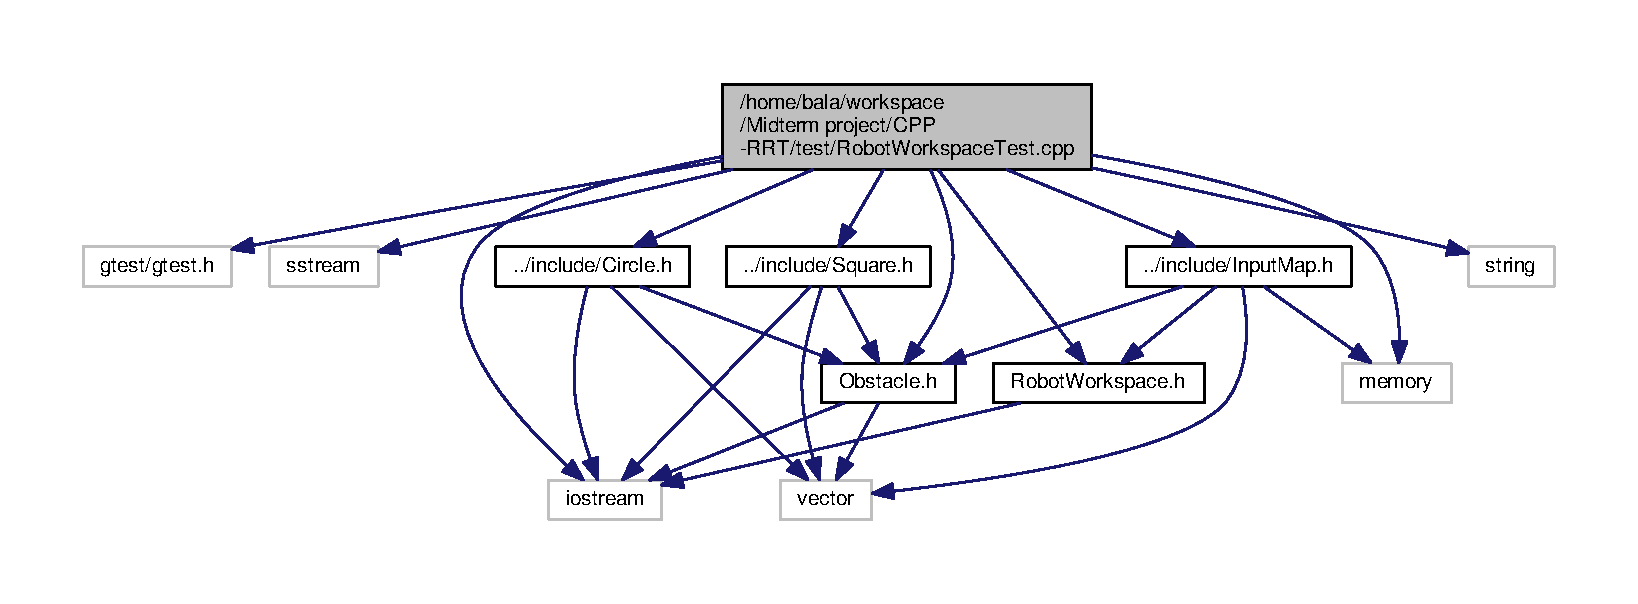
\includegraphics[width=350pt]{RobotWorkspaceTest_8cpp__incl}
\end{center}
\end{figure}
\subsection*{Classes}
\begin{DoxyCompactItemize}
\item 
struct \hyperlink{structRobotWorkspaceTest}{Robot\+Workspace\+Test}
\begin{DoxyCompactList}\small\item\em \hyperlink{classRobotWorkspace}{Robot\+Workspace} class test fixture. \end{DoxyCompactList}\end{DoxyCompactItemize}
\subsection*{Functions}
\begin{DoxyCompactItemize}
\item 
\hyperlink{RobotWorkspaceTest_8cpp_a0a0426e2529d6aaad45e2d9fde531203}{T\+E\+ST} (Robot\+Work\+Space\+Class, Initialization)
\begin{DoxyCompactList}\small\item\em Testing \hyperlink{classRobotWorkspace}{Robot\+Workspace} initialization. \end{DoxyCompactList}\item 
\hyperlink{RobotWorkspaceTest_8cpp_a2f5d025e7e02b572b7d0c565860d48dd}{T\+E\+S\+T\+\_\+F} (\hyperlink{structRobotWorkspaceTest}{Robot\+Workspace\+Test}, Compute\+And\+Get\+Methods)
\begin{DoxyCompactList}\small\item\em Testing if point is inside square obstacle or not. \end{DoxyCompactList}\end{DoxyCompactItemize}


\subsection{Function Documentation}
\index{Robot\+Workspace\+Test.\+cpp@{Robot\+Workspace\+Test.\+cpp}!T\+E\+ST@{T\+E\+ST}}
\index{T\+E\+ST@{T\+E\+ST}!Robot\+Workspace\+Test.\+cpp@{Robot\+Workspace\+Test.\+cpp}}
\subsubsection[{\texorpdfstring{T\+E\+S\+T(\+Robot\+Work\+Space\+Class, Initialization)}{TEST(RobotWorkSpaceClass, Initialization)}}]{\setlength{\rightskip}{0pt plus 5cm}T\+E\+ST (
\begin{DoxyParamCaption}
\item[{Robot\+Work\+Space\+Class}]{, }
\item[{Initialization}]{}
\end{DoxyParamCaption}
)}\hypertarget{RobotWorkspaceTest_8cpp_a0a0426e2529d6aaad45e2d9fde531203}{}\label{RobotWorkspaceTest_8cpp_a0a0426e2529d6aaad45e2d9fde531203}


Testing \hyperlink{classRobotWorkspace}{Robot\+Workspace} initialization. 

\index{Robot\+Workspace\+Test.\+cpp@{Robot\+Workspace\+Test.\+cpp}!T\+E\+S\+T\+\_\+F@{T\+E\+S\+T\+\_\+F}}
\index{T\+E\+S\+T\+\_\+F@{T\+E\+S\+T\+\_\+F}!Robot\+Workspace\+Test.\+cpp@{Robot\+Workspace\+Test.\+cpp}}
\subsubsection[{\texorpdfstring{T\+E\+S\+T\+\_\+\+F(\+Robot\+Workspace\+Test, Compute\+And\+Get\+Methods)}{TEST_F(RobotWorkspaceTest, ComputeAndGetMethods)}}]{\setlength{\rightskip}{0pt plus 5cm}T\+E\+S\+T\+\_\+F (
\begin{DoxyParamCaption}
\item[{{\bf Robot\+Workspace\+Test}}]{, }
\item[{Compute\+And\+Get\+Methods}]{}
\end{DoxyParamCaption}
)}\hypertarget{RobotWorkspaceTest_8cpp_a2f5d025e7e02b572b7d0c565860d48dd}{}\label{RobotWorkspaceTest_8cpp_a2f5d025e7e02b572b7d0c565860d48dd}


Testing if point is inside square obstacle or not. 


\hypertarget{RRTTest_8cpp}{}\section{/home/bala/workspace/\+Midterm project/\+C\+P\+P-\/\+R\+R\+T/test/\+R\+R\+T\+Test.cpp File Reference}
\label{RRTTest_8cpp}\index{/home/bala/workspace/\+Midterm project/\+C\+P\+P-\/\+R\+R\+T/test/\+R\+R\+T\+Test.\+cpp@{/home/bala/workspace/\+Midterm project/\+C\+P\+P-\/\+R\+R\+T/test/\+R\+R\+T\+Test.\+cpp}}
{\ttfamily \#include $<$gtest/gtest.\+h$>$}\\*
{\ttfamily \#include $<$memory$>$}\\*
{\ttfamily \#include $<$iostream$>$}\\*
{\ttfamily \#include $<$utility$>$}\\*
{\ttfamily \#include $<$vector$>$}\\*
{\ttfamily \#include \char`\"{}../include/\+Input\+Map.\+h\char`\"{}}\\*
{\ttfamily \#include \char`\"{}../include/\+R\+R\+T.\+h\char`\"{}}\\*
{\ttfamily \#include \char`\"{}../include/\+Square.\+h\char`\"{}}\\*
Include dependency graph for R\+R\+T\+Test.\+cpp\+:
\nopagebreak
\begin{figure}[H]
\begin{center}
\leavevmode
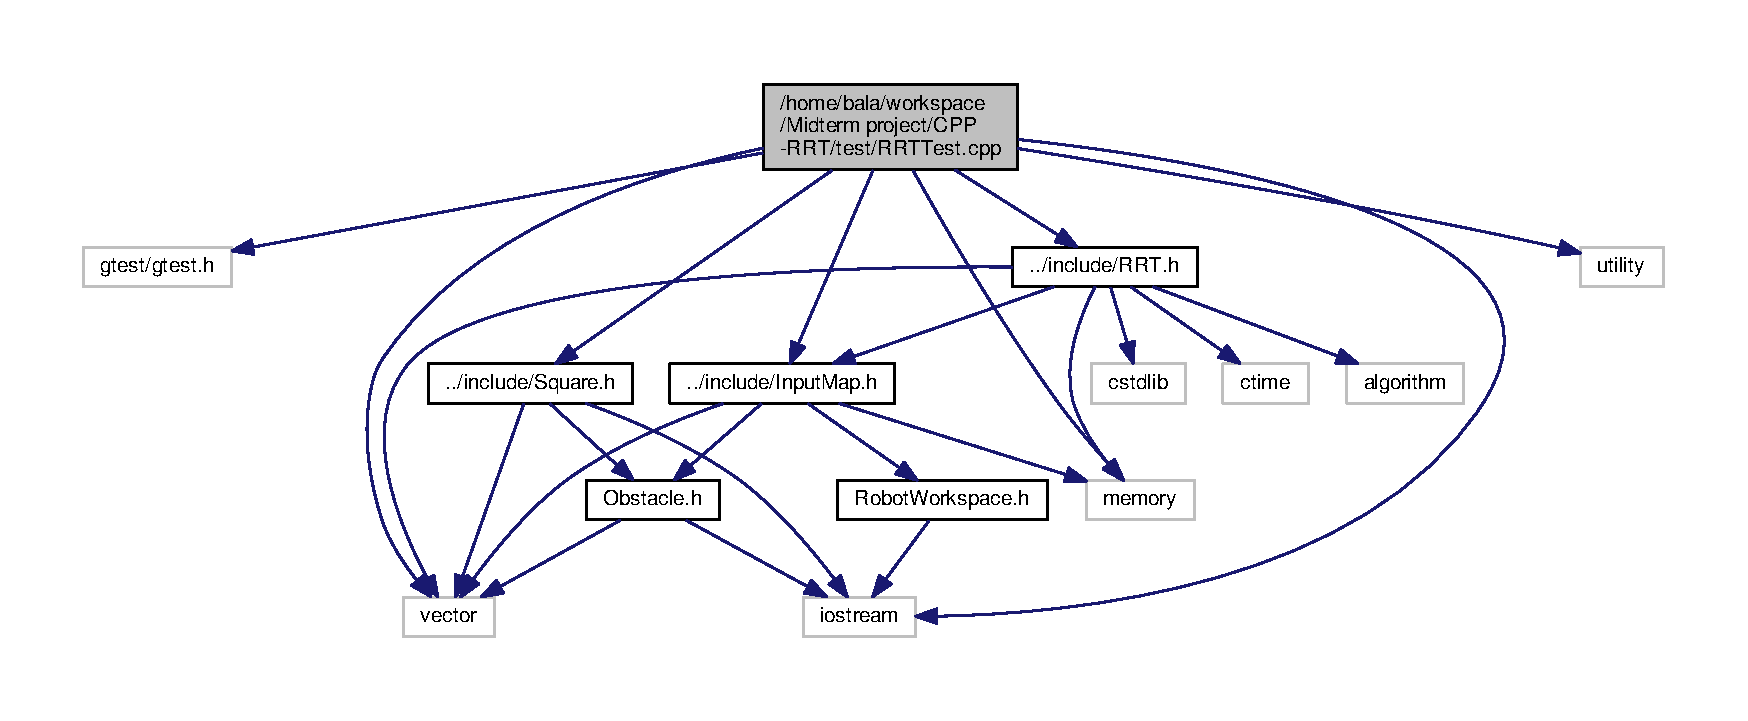
\includegraphics[width=350pt]{RRTTest_8cpp__incl}
\end{center}
\end{figure}
\subsection*{Functions}
\begin{DoxyCompactItemize}
\item 
\hyperlink{RRTTest_8cpp_a3d777d230ee0026bf73280842147bea3}{T\+E\+ST} (R\+R\+T\+Class, is\+Goal\+In\+Tree)
\end{DoxyCompactItemize}


\subsection{Function Documentation}
\index{R\+R\+T\+Test.\+cpp@{R\+R\+T\+Test.\+cpp}!T\+E\+ST@{T\+E\+ST}}
\index{T\+E\+ST@{T\+E\+ST}!R\+R\+T\+Test.\+cpp@{R\+R\+T\+Test.\+cpp}}
\subsubsection[{\texorpdfstring{T\+E\+S\+T(\+R\+R\+T\+Class, is\+Goal\+In\+Tree)}{TEST(RRTClass, isGoalInTree)}}]{\setlength{\rightskip}{0pt plus 5cm}T\+E\+ST (
\begin{DoxyParamCaption}
\item[{R\+R\+T\+Class}]{, }
\item[{is\+Goal\+In\+Tree}]{}
\end{DoxyParamCaption}
)}\hypertarget{RRTTest_8cpp_a3d777d230ee0026bf73280842147bea3}{}\label{RRTTest_8cpp_a3d777d230ee0026bf73280842147bea3}

%--- End generated contents ---

% Index
\backmatter
\newpage
\phantomsection
\clearemptydoublepage
\addcontentsline{toc}{chapter}{Index}
\printindex

\end{document}
